% Options for packages loaded elsewhere
\PassOptionsToPackage{unicode}{hyperref}
\PassOptionsToPackage{hyphens}{url}
%
\documentclass[
]{article}
\usepackage{amsmath,amssymb}
\usepackage{iftex}
\ifPDFTeX
  \usepackage[T1]{fontenc}
  \usepackage[utf8]{inputenc}
  \usepackage{textcomp} % provide euro and other symbols
\else % if luatex or xetex
  \usepackage{unicode-math} % this also loads fontspec
  \defaultfontfeatures{Scale=MatchLowercase}
  \defaultfontfeatures[\rmfamily]{Ligatures=TeX,Scale=1}
\fi
\usepackage{lmodern}
\ifPDFTeX\else
  % xetex/luatex font selection
\fi
% Use upquote if available, for straight quotes in verbatim environments
\IfFileExists{upquote.sty}{\usepackage{upquote}}{}
\IfFileExists{microtype.sty}{% use microtype if available
  \usepackage[]{microtype}
  \UseMicrotypeSet[protrusion]{basicmath} % disable protrusion for tt fonts
}{}
\makeatletter
\@ifundefined{KOMAClassName}{% if non-KOMA class
  \IfFileExists{parskip.sty}{%
    \usepackage{parskip}
  }{% else
    \setlength{\parindent}{0pt}
    \setlength{\parskip}{6pt plus 2pt minus 1pt}}
}{% if KOMA class
  \KOMAoptions{parskip=half}}
\makeatother
\usepackage{xcolor}
\usepackage[margin=1in]{geometry}
\usepackage{color}
\usepackage{fancyvrb}
\newcommand{\VerbBar}{|}
\newcommand{\VERB}{\Verb[commandchars=\\\{\}]}
\DefineVerbatimEnvironment{Highlighting}{Verbatim}{commandchars=\\\{\}}
% Add ',fontsize=\small' for more characters per line
\usepackage{framed}
\definecolor{shadecolor}{RGB}{248,248,248}
\newenvironment{Shaded}{\begin{snugshade}}{\end{snugshade}}
\newcommand{\AlertTok}[1]{\textcolor[rgb]{0.94,0.16,0.16}{#1}}
\newcommand{\AnnotationTok}[1]{\textcolor[rgb]{0.56,0.35,0.01}{\textbf{\textit{#1}}}}
\newcommand{\AttributeTok}[1]{\textcolor[rgb]{0.13,0.29,0.53}{#1}}
\newcommand{\BaseNTok}[1]{\textcolor[rgb]{0.00,0.00,0.81}{#1}}
\newcommand{\BuiltInTok}[1]{#1}
\newcommand{\CharTok}[1]{\textcolor[rgb]{0.31,0.60,0.02}{#1}}
\newcommand{\CommentTok}[1]{\textcolor[rgb]{0.56,0.35,0.01}{\textit{#1}}}
\newcommand{\CommentVarTok}[1]{\textcolor[rgb]{0.56,0.35,0.01}{\textbf{\textit{#1}}}}
\newcommand{\ConstantTok}[1]{\textcolor[rgb]{0.56,0.35,0.01}{#1}}
\newcommand{\ControlFlowTok}[1]{\textcolor[rgb]{0.13,0.29,0.53}{\textbf{#1}}}
\newcommand{\DataTypeTok}[1]{\textcolor[rgb]{0.13,0.29,0.53}{#1}}
\newcommand{\DecValTok}[1]{\textcolor[rgb]{0.00,0.00,0.81}{#1}}
\newcommand{\DocumentationTok}[1]{\textcolor[rgb]{0.56,0.35,0.01}{\textbf{\textit{#1}}}}
\newcommand{\ErrorTok}[1]{\textcolor[rgb]{0.64,0.00,0.00}{\textbf{#1}}}
\newcommand{\ExtensionTok}[1]{#1}
\newcommand{\FloatTok}[1]{\textcolor[rgb]{0.00,0.00,0.81}{#1}}
\newcommand{\FunctionTok}[1]{\textcolor[rgb]{0.13,0.29,0.53}{\textbf{#1}}}
\newcommand{\ImportTok}[1]{#1}
\newcommand{\InformationTok}[1]{\textcolor[rgb]{0.56,0.35,0.01}{\textbf{\textit{#1}}}}
\newcommand{\KeywordTok}[1]{\textcolor[rgb]{0.13,0.29,0.53}{\textbf{#1}}}
\newcommand{\NormalTok}[1]{#1}
\newcommand{\OperatorTok}[1]{\textcolor[rgb]{0.81,0.36,0.00}{\textbf{#1}}}
\newcommand{\OtherTok}[1]{\textcolor[rgb]{0.56,0.35,0.01}{#1}}
\newcommand{\PreprocessorTok}[1]{\textcolor[rgb]{0.56,0.35,0.01}{\textit{#1}}}
\newcommand{\RegionMarkerTok}[1]{#1}
\newcommand{\SpecialCharTok}[1]{\textcolor[rgb]{0.81,0.36,0.00}{\textbf{#1}}}
\newcommand{\SpecialStringTok}[1]{\textcolor[rgb]{0.31,0.60,0.02}{#1}}
\newcommand{\StringTok}[1]{\textcolor[rgb]{0.31,0.60,0.02}{#1}}
\newcommand{\VariableTok}[1]{\textcolor[rgb]{0.00,0.00,0.00}{#1}}
\newcommand{\VerbatimStringTok}[1]{\textcolor[rgb]{0.31,0.60,0.02}{#1}}
\newcommand{\WarningTok}[1]{\textcolor[rgb]{0.56,0.35,0.01}{\textbf{\textit{#1}}}}
\usepackage{longtable,booktabs,array}
\usepackage{calc} % for calculating minipage widths
% Correct order of tables after \paragraph or \subparagraph
\usepackage{etoolbox}
\makeatletter
\patchcmd\longtable{\par}{\if@noskipsec\mbox{}\fi\par}{}{}
\makeatother
% Allow footnotes in longtable head/foot
\IfFileExists{footnotehyper.sty}{\usepackage{footnotehyper}}{\usepackage{footnote}}
\makesavenoteenv{longtable}
\usepackage{graphicx}
\makeatletter
\def\maxwidth{\ifdim\Gin@nat@width>\linewidth\linewidth\else\Gin@nat@width\fi}
\def\maxheight{\ifdim\Gin@nat@height>\textheight\textheight\else\Gin@nat@height\fi}
\makeatother
% Scale images if necessary, so that they will not overflow the page
% margins by default, and it is still possible to overwrite the defaults
% using explicit options in \includegraphics[width, height, ...]{}
\setkeys{Gin}{width=\maxwidth,height=\maxheight,keepaspectratio}
% Set default figure placement to htbp
\makeatletter
\def\fps@figure{htbp}
\makeatother
\ifLuaTeX
  \usepackage{luacolor}
  \usepackage[soul]{lua-ul}
\else
  \usepackage{soul}
\fi
\setlength{\emergencystretch}{3em} % prevent overfull lines
\providecommand{\tightlist}{%
  \setlength{\itemsep}{0pt}\setlength{\parskip}{0pt}}
\setcounter{secnumdepth}{5}
\ifLuaTeX
  \usepackage{selnolig}  % disable illegal ligatures
\fi
\usepackage{bookmark}
\IfFileExists{xurl.sty}{\usepackage{xurl}}{} % add URL line breaks if available
\urlstyle{same}
\hypersetup{
  pdftitle={Fundamentos de Inferencia Estadistica},
  pdfauthor={Alex Sanchez Pla y Santiago Pérez Hoyos},
  hidelinks,
  pdfcreator={LaTeX via pandoc}}

\title{Fundamentos de Inferencia Estadistica}
\author{Alex Sanchez Pla y Santiago Pérez Hoyos}
\date{2024-10-21}

\begin{document}
\maketitle

{
\setcounter{tocdepth}{2}
\tableofcontents
}
\section*{Presentación}\label{presentaciuxf3n}
\addcontentsline{toc}{section}{Presentación}

\subsection*{Objetivo}\label{objetivo}
\addcontentsline{toc}{subsection}{Objetivo}

El objetivo de estas notas es presentar un material de soporte para la asignatura de ``Inferencia Estadística'' del \href{https://www.uoc.edu/es/estudios/masters/master-universitario-bioinformatica-bioestadistica}{Máster interuniversitario de Bioiestadística y Bioinformática} impartido conjuntamente por la \href{https://www.uoc.edu}{Universitat Oberta de Catalunya (UOC)} y la \href{https://www.ub.edu}{Universidad de Barcelona (UB)}.

Esta asignatura adolece de las características habituales de las asignaturas de posgrado, y especialmente de un posgrado de estadística (y bioinformática), que muestran algunas de las cosas que no debe de ser esta asignatura:

\begin{itemize}
\tightlist
\item
  No puede ser un primer curso de estadística, porque se supone que los estudiantes del máster ya lo han cursado en sus grados. Por no decir que, a quien viene a especializarse en estadística se le puede suponer una base mínima.
\item
  Tampoco debe ser como los segundos cursos de estadística de algunos grados, que tratan temas como la regresión, el diseño de experimentos o el análisis multivariante, porque esto ya se trata en diversas asignaturas del máster.
\end{itemize}

¿Que debemos pues esperar que sea este curso?

\begin{itemize}
\tightlist
\item
  Puestos a pedir, este curso debería servir para repasar y consolidar los conceptos básicos que la mayoría de estudiantes traerán consigo.
\item
  Además, y sobretodo, debe proporcionar una visión general, lo más completa posible dentro de las limitaciones de tiempo, del campo de la inferencia estadística
\item
  Y, naturalmente, esto significa proporcionar aquellos conceptos sobre los que se apoyaran muchas de las restantes asignaturas como ``Regresión modelos y métodos'', ``Diseño de Experimentos'', ``Análisis Multivariante'', ``Análisis de la Supervivencia'' o ``Análisis de datos ómicos''.
\end{itemize}

\subsection*{Prerequisitos y organización del material}\label{prerequisitos-y-organizaciuxf3n-del-material}
\addcontentsline{toc}{subsection}{Prerequisitos y organización del material}

Uno de los problemas ``eternos'' en el estudio de la estadística ha sido siempre la falta de acuerdo, entre la comunidad de docentes, de cual debería ser el nivel matemático a que se impartan los cursos.

En los cursos de pre-grado ha habido un cierto consenso, y con los años el nivel de formalismo ha disminuido, incluso en estudios de tipo ``STEM'', tendiendo a centrarse en la aplicación de los conceptos, por ejemplo usando R, más que en un tratamiento formal (``matemático'') de los mismos.

Aunque esto puede ser práctico para aquellos estudios en los que la estadística és una asignatura de un grado, es también obvio que dicha aproximación no permite profundizar en muchos de los puntos que se tratan.

Es por ello que en este curso seguiremos la indicación habitual en cursos similares de asumir que el estudiante:

\begin{itemize}
\tightlist
\item
  Se siente comodo con el lenguaje algebráico, desarrollo de expresiones, sumatorios etc.
\item
  Está familiarizado con el cálculo diferencial en una o varias variables, aunque esta familiaridad no será imprescindible para seguir la mayoría de los contenidos del curso.
\item
  Conoce el lenguaje estadístico R, que en muchas ocasiones nos ofrecerá una solución directa a los problemas de cálculo.
\end{itemize}

\subsection*{Referencias}\label{referencias}
\addcontentsline{toc}{subsection}{Referencias}

Los prerequisitos anteriores corresponden básicamente a las matemáticas del bachilerato. Algunas funetes adiconales pueden ser:

\begin{itemize}
\item
  \href{http://cimanet.uoc.edu/cursMates0/IniciacionMatematicas/pdf/PID_00273914.pdf}{Iniciación a las matemáticas para la ingeniería. M. Besalú y Joana Villalonga}

  \begin{itemize}
  \tightlist
  \item
    \href{https://www.youtube.com/playlist?list=PLv8FweHfYYMo6Lr2zt6H4znq5KuBacq28}{Colección de (100) videos de soporte a las matemáticas para la ingeniería}
  \end{itemize}
\end{itemize}

\section*{Agradecimiento y fuentes utilizadas}\label{agradecimiento-y-fuentes-utilizadas}
\addcontentsline{toc}{section}{Agradecimiento y fuentes utilizadas}

Salvo que uno desee escribir un libro sobre algo muy extraño, siempre habran otros libros o manuales similares al que se está planteando.

La respuesta a la pregunta, ``Y entonces, ¿porque hacer un nuevo matrerial?'' suele ser más una excusa que una explicación sólida.

Una posible razón puede ser \emph{para ajustarlo al máximo al perfil del curso para al que se destinan dichos materiales}, condición que otros textos, pensados para cursos y audiencias distintas, pueden no satisfacer. En este caso adoptaremos esta explicación y el tiempo decidirá si el objetivo se alcanza.

Dicho esto, debemos agradecer a las distintas fuentes utilizadas, el que hayan puesto a disposición sus materiales para poder reutilizarlos. Entre estos destacamos:

\subsection*{El proyecto Statmedia}\label{el-proyecto-statmedia}
\addcontentsline{toc}{subsection}{El proyecto Statmedia}

Statmedia es un grupo de innovación docente de la Universidad de Barcelona, cuyo objetivo es desarrollar nuevas herramientas que ayuden en la enseñanza de la estadística aplicada, mejorando así el rendimiento académico de los alumnos y su motivación hacia la estadística.

Partiendo de la idea que el aprendizaje debe basarse en casos prácticos para motivar y fomentar la participación de los estudiantes. Se desarrolló primer proyecto, Statmedia I, un texto multimedia de estadística que además de los contenidos, relativamente ampliados, para un curso de introducción a la estadística, incorporaba:

\begin{itemize}
\tightlist
\item
  Una serie de casos para motivar e ilustrar los conceptos introducidos.
\item
  Un conjunto de gadgets interactivos con los que interactuar y experimentar y
\item
  Ejercicios de respuesta múltiple para verificar los conceptos trabajados.
\end{itemize}

Aunque el proyecto Statmedia ha seguido evolucionando en múltiples direcciones, Statmedia I, como tantos otros, no sobrevivió al desarrollo tecnológico, y la evolución (o decadencia) del lenguaje Java lo llevó a dejar de ser funcional.

Para estos apuntes hemos recuperado, y en ocasiones adaptado o modificado, algunos de los contenidos de Statmedia I, que habían estado escritos con gran pulcritud. Esto se ha hecho siguiendo las indicaciones de la licencia (CC-Share-alike) que permite adaptar contenidos atribuyendolo a sus autores y citando la fuente.

Los gadgets originales ya no son funcionales pero muchos de ellos han sido re-escritos en R como aplicaciones Shiny (disponibles en: \url{https://grbio.upc.edu/en/software/teaching_apps}) y se enlazaran desde los puntos necesarios del texto.

Dejando aparte (además) de la licencia, vaya nuestro agradecimiento explícito al equipo de profesores del Departamento de Estadística de la Universidad de Barcelona, redactor de la versión inicial del proyecto, que es la que hemos utilizado: Antonio Arcas Pons, Miquel calvo Llorca, Antonio Miñarro Alonso, Sergi Civit Vives y Angel Vilarroya del Campo.

\href{https://www.emis.de/journals/BEIO/files/BEIOv25n1_HE_A.Arcas+A.Minarro+M.Calvo.pdf}{Antoni Arcas, Antonio Miñarro and Miguel Calvo (2008) Statmedia projects in Statistical Education}

\subsection*{Otros materiales utilizados}\label{otros-materiales-utilizados}
\addcontentsline{toc}{subsection}{Otros materiales utilizados}

\begin{itemize}
\item
  \href{https://github.com/ASPteaching/ApuntsEstadisticaMatematica}{Alex Sanchez y Francesc Carmona (2002). Apunts d'Estadística Matemàtica} Licencia CC0 1.0 Universal
\item
  \href{https://bookdown.org/egarpor/inference/}{Molina Peralta, I. and García-Portugués, E. (2024). \emph{A First Course on Statistical Inference}. Version 2.4.1. ISBN 978-84-09-29680-4}. Licencia CC BY-NC-ND 4.0
\item
  \href{https://bookdown.org/pkaldunn/DistTheory}{Peter K. Dunn (2024) \emph{The theory of distributions}.} Licencia CC BY-NC-ND 4.0
\end{itemize}

\section{Probabilidad y Experimentos aleatorios}\label{probabilidad-y-experimentos-aleatorios}

\subsection{Introducción}\label{introducciuxf3n}

\subsubsection{Fenómenos deterministas y fenómenos aleatorios}\label{fenuxf3menos-deterministas-y-fenuxf3menos-aleatorios}

Supongamos que disponemos de un dado regular con todas las caras
pintadas de blanco y con un número, que irá de 1 a \(6 \sin\) repetir
ninguno, en cada una de las seis caras.

Definamos los dos experimentos siguientes: Experimento 1: Tirar el dado
y anotar el color de la cara resultante. Experimento 2: Tirar el dado y
anotar el número de la cara resultante. ¿Qué diferencia fundamental
observamos entre ambos experimentos? Muy simple! En el experimento 1, el
resultado es obvio: saldrá una cara de color blanco. Es decir, es
posible predecir el resultado. Se trata de un experimento o fenómeno
determinista.

En cambio, en el experimento 2 no podemos predecir cuál será el valor
resultante. El resultado puede ser : \(1,2,3,4,5\) o 6 . Se trata de un
experimento o fenómeno aleatorio.

El conjunto de resultados se anotará con el símbolo: \(\Omega\). En este
caso, \(\Omega=\{1,2,3,4,5,6\}\). En los fenómenos aleatorios, al hacer
muchas veces la experiencia, la frecuencia relativa de cualquier
elemento del conjunto de resultados debe aproximarse siempre hacia un
mismo valor.

\subsubsection{Sucesos}\label{sucesos}

Supongamos que se ejecuta un experimento aleatorio. Se nos puede ocurrir
emitir un enunciado que, una vez realizada la experiencia, pueda decirse
si se ha verificado o no se ha verificado. A dichos enunciados los
denominamos sucesos.

Por otro lado, los sucesos van asociados a subconjuntos del conjunto de
resultados. Cada suceso se corresponderá exactamente con uno, y sólo con
un, subconjunto del conjunto de resultados.

Veamos un ejemplo: Experimento: Tirar un dado regular. Conjunto de
resultados : \(\Omega=\{1,2,3,4,5,6\}\) Enunciado: Obtener múltiplo de 3.
Subconjunto al que se asocia el enunciado: \(A=\{3,6\}\) Nos referiremos
habitualmente al suceso A.

\paragraph{Sucesos y conjuntos}\label{sucesos-y-conjuntos}

Al conjunto de resultados \(\Omega\), se le denomina suceso seguro. Al
conjunto Ø ( conjunto sin elementos), se le denomina suceso imposible.
Al complementario del conjunto
\(\mathrm{A}\left(\mathrm{A}^{\mathrm{c}}\right)\), se le denomina suceso
contrario o complementario de \(A\). A partir de dos sucesos A y B,
podemos formar los sucesos siguientes:

\begin{itemize}
\tightlist
\item
  A intersección B, que anotaremos como:
\end{itemize}

\[
A \cap B
\]

\begin{itemize}
\tightlist
\item
  A unión B, que anotaremos como:
\end{itemize}

\[
A \cup B
\]

A intersección B, significa que se verifican a la vez A y B. A unión B,
significa que se verifica \(A\) o \(B\) ( se pueden verificar a la vez).

\subsection{Función de probabilidad}\label{funciuxf3n-de-probabilidad}

Lógicamente, una vez tenemos un suceso, nos preocupa saber si hay muchas
o pocas posibilidades de que al realizar la experiencia se haya
verificado.

Por lo tanto, sería interesante el tener alguna función que midiera el
grado de confianza a depositar en que se verifique el suceso.

A esta función la denominaremos función de probabilidad. La función de
probabilidad será, pues, una aplicación entre el conjunto de resultados
y el conjunto de números reales, que asignará a cada suceso la
probabilidad de que se verifique.

La notación: \(\mathrm{P}(\mathrm{A})\) significará: probabilidad de que
se verifique el suceso A . Pero claro, de funciones de probabilidad
asociadas a priori a una experiencia aleatoria podrían haber muchas.

Lo que se hace para decir qué es y qué no es una función de probabilidad
es construir una serie de propiedades (denominadas axiomas) que se
exigirán a una función para poder ser catalogada como función de
probabilidad.

Y, ¿cuáles son estos axiomas? Pues los siguientes: Sea S el conjunto de
sucesos.

\begin{itemize}
\item
  Axioma 1: Para cualquier suceso A, la probabilidad debe ser
  mayor o igual que 0.
\item
  Axioma 2: La probabilidad del \emph{suceso seguro} debe ser 1: \(\mathrm{P}(\Omega)=1\)
\item
  Axioma 3: Para sucesos \(\mathrm{A}_{\mathrm{i}}\), de modo que cada par de sucesos no
  tengan ningún resultado común, se verifica que:
\end{itemize}

\[
P\left(\bigcup_{i=1}^{\infty} A_{i}\right)=\sum_{i=1}^{\infty} P\left(A_{i}\right)
\]

De este modo, pueden haber muchas funciones de probabilidad que se
podrían asociar con la experiencia.

El problema pasa entonces al investigador para decidir cual o cuales son
las funciones de probabilidad más razonables asociadas con la
experiencia que está manejando.

\subsubsection{¿Diferentes funciones de probabilidad para una misma experiencia aleatoria?}\label{diferentes-funciones-de-probabilidad-para-una-misma-experiencia-aleatoria}

Supongamos la experiencia de tirar un dado regular. A todo el mundo se
le ocurriría pensar que la función de probabilidad se obtiene de contar
el número de resultados que contiene el suceso dividido por 6 , que es
el número total de resultados posibles. Así pues, la probabilidad de
obtener un múltiplo de 3 sería igual a \(2 / 6\), la probabilidad de
obtener el número 2 sería \(1 / 6\) i la probabilidad de obtener un número
par sería 3/6. Es decir, parece inmediato construir la función de
probabilidad que, además, parece única. A nadie se le ocurre decir, por
ejemplo, que la probabilidad de obtener un número par es \(5 / 6\) !

En este caso, todo ha sido muy fácil. Hemos visto que existe una única
función de probabilidad que encaje de forma lógica con la experiencia y,
además, ha sido muy sencillo encontrarla.

Pero esto, por desgracia, no siempre es así. En muchísimas ocasiones
resulta muy complejo el decidir cuál es la función de probabilidad.

En el tema de variables aleatorias y de función de distribución se
explica el problema de la modelización de muchas situaciones reales.

\subsection{¿Cómo se calculan las probabilidades?}\label{cuxf3mo-se-calculan-las-probabilidades}

No siempre es fácil conocer los valores de la función de probabilidad de
todos los sucesos. Sin embargo, muchas veces se pueden conocer las
probabilidades de algunos de estos sucesos. Con la ayuda de ciertas
propiedades que se deducen de manera inmediata a partir de la axiomática
es posible calcular las probabilidades de más sucesos.

Por otro lado, en caso de que el número de resultados sea finito y de
que todos los resultados tengan las mismas posibilidades de verificarse,
la probabilidad de un suceso cualquiera se puede calcular a partir de la
regla de Laplace:

Si A es un suceso :

\[
\text { Probabilidad }(A)=\frac{\text { Número de casos favorables }}{\text { Número de casos posibles }}
\]

donde: Número de casos favorables \(=\) Número de resultados contenidos en
\(\mathrm{A}(\) cardinal de A\()\) Número de casos posibles \(=\) Número total
de resultados posibles (cardinal del conjunto total de resultados)

En este caso, el contar número de resultados, ya sean favorables o
posibles, debe hacerse por medio de la combinatoria.

Veamos con unos ejemplos muy sencillos y visuales cómo se obtienen y qué
representan los casos posibles y los casos favorables.

También es posible obtener de manera aproximada la probabilidad de un
suceso si se puede repetir muchas veces la experiencia: la probabilidad
del suceso sería el valor al que tendería la frecuencia relativa del
suceso. Podéis consultar más detalles acerca de esta aproximación.

En este caso, la cuestión estriba en poder hacer muchas veces la
experiencia en condiciones independientes.

\subsection{Sucesos elementales y sucesos observables}\label{sucesos-elementales-y-sucesos-observables}

En el contexto de la probabilidad, es fundamental diferenciar entre los \textbf{sucesos elementales} y los \textbf{sucesos observables}.

Los sucesos elementales son los resultados individuales que pueden ocurrir al realizar un experimento aleatorio, es decir, cada uno de los elementos que conforman el conjunto de resultados \(\Omega\). En nuestro ejemplo del dado, los sucesos elementales son los números \(1, 2, 3, 4, 5\) y \(6\).

Sin embargo, no todos los sucesos elementales son necesariamente observables. Un suceso observable es un subconjunto de estos sucesos elementales que permite formular afirmaciones verificables sobre el resultado del experimento.

\textbf{Ejemplo}

\begin{enumerate}
\def\labelenumi{\arabic{enumi}.}
\item
  Podemos imaginar un dado en el que pintamos de blanco las caras pares y de negro las impares. En este caso los sucesos elementales serían los habituales 1, 2, 3,\ldots6.
  Sin embargo tan solo ``Par'' (``blanco'') o impar (``negro'') se pueden observar.
\item
  Si repintamos el dado de forma que las caras 1 y 2 esten blancas, las 3 y 4, azules y las 5 y 6 rojas podremos observar el suceso ``Sale 1 o 2 (=Sale blanco)'' o ``sale blanco o azul'', pero no el suceso ``sale par'' dado que cada color contiene un número par y uno impar
\end{enumerate}

Para formalizar estos conceptos, definimos el \textbf{espacio de probabilizable} como el par de conjuntos formados por: \((\Omega, \mathcal{A})\)

\begin{itemize}
\tightlist
\item
  \(\Omega\) es el conjunto de todos los resultados posibles (el conjunto de resultados o sucesos elementales).
\item
  \(\mathcal{A}\) es el conjunto de todos los sucesos observables, que vienen definidos por el \emph{nivel de observación} del experimento.
\end{itemize}

\subsection{Propiedades inmediatas de la probabilidad}\label{propiedades-inmediatas-de-la-probabilidad}

Veremos a continuación una serie de propiedades que se deducen de manera
inmediata de la axiomática de la probabilidad.

\subsubsection{Succeso imposible}\label{succeso-imposible}

El suceso imposible se identifica con el conjunto vacío, puesto que no hay ningún resultado asociado a él. La probabilidad del suceso imposible es:

\[
P(\varnothing)=0
\]

\subsubsection{Suceso implicado}\label{suceso-implicado}

Decimos que un suceso, B, esta implicado por otro suceso A, si siempre que se presenta A, también lo hace B. Por ejemplo, si al tirar un dado se obtiene un dos (suceso A), ello implica que ha salido un número par (suceso B). En terminos de conjuntos, A es un suceso que está contenido en B (todos los resultados de A
también pertenecen a B ), por lo que:

\[
\mathrm{P}(\mathrm{A}) \leq \mathrm{P}(\mathrm{B})
\]

\subsubsection{Complementario de un suceso}\label{complementario-de-un-suceso}

Sea \(A^{\mathrm{c}}\) el suceso formado por todos los elementos de
\(\Omega\) que no pertenecen a A (Suceso complementario de A). La
probabilidad de dicho suceso es igual a:

\[
\mathrm{P}\left(\mathrm{A}^{\mathrm{c}}\right)=1-\mathrm{P}(\mathrm{A})
\]

\subsubsection{Ocurrencia de algun suceso}\label{ocurrencia-de-algun-suceso}

La probabilidad de la unión de dos sucesos A y B es igual a:

\[
P(A \cup B)=P(A)+P(B)-P(A \cap B)
\]

\subsubsection{Probabilidad de que ocurra algun suceso}\label{probabilidad-de-que-ocurra-algun-suceso}

Si tenemos una colección de \(k\) sucesos, la probabilidad de la unión de
dichos sucesos será:

\[
P\left(\bigcup_{i=1}^{k} A_{i}\right)=\sum_{i=1}^{k} P\left(A_{i}\right)-\sum_{i<j} P\left(A_{i} \cap A_{j}\right)+\sum P\left(A_{i} \cap A_{j} \cap A_{k}\right)+\ldots+(-1)^{k+1} \cdot P\left(A_{1} \cap . . \cap A_{k}\right)
\]

\subsubsection{Probabilidad de que ocurran dos (o más) sucesos a la vez}\label{probabilidad-de-que-ocurran-dos-o-muxe1s-sucesos-a-la-vez}

No existe una expresión cerrada única para la probabilidad de que ocurran dos o más sucesos a la vez, pues esto depende de si los sucesos que consideramos son dependientes o independientes, conceptos éstos, que introduciremos en la próxima sección.

Lo que si que existe es una cota para dicha probabilidad, es decir, podemos decir que valor alcanza dicha probabilidad, \emph{como mínimo}.

\[
P\left(\bigcap_{i=1}^{n} A_{i}\right) \geq 1-\sum_{i=1}^{n} P\left(\bar{A}_{i}\right)
\]

\subsection{Espacios de probabilidad}\label{espacios-de-probabilidad}

Para concluir esta introducción introduciremos los \textbf{espacio de probabilidad} que, extienden los \textbf{espacios probabilizables} definidos en la sección anterior

La terna \((\Omega, \mathcal{A}, P)\) donde:

\begin{itemize}
\tightlist
\item
  \(Omega\) es el conjunto de todos los resultados posibles (el conjunto de resultados o sucesos elementales),
\item
  \(\mathcal{A}\) es el conjunto de todos los sucesos observables, que vienen definidos por el \emph{nivel de observación} del experimento y
\item
  \(P\) es una función de probabilidad, que asigna a cada suceso observable \(A \in \mathcal{A}\) un número real \(P(A)\) que representa la probabilidad de que ocurra dicho suceso
\end{itemize}

se conoce como \textbf{espacio de probabilidad}.

Es importante destacar que \textbf{la probabilidad se calcula exclusivamente para los sucesos observables}, lo que garantiza que la medida sea coherente y verificada a través de experimentos.

Los espacios de probabilidad proporcionan una estructura fundamental para analizar y medir las incertidumbres asociadas a los fenómenos aleatorios, facilitando el estudio de sus propiedades, la construcción, sobre ellos de diversos conceptos fundamentales como el de variables aleatorias, y, en general, la aplicación de teorías de la probabilidad a diversas áreas de conocimiento.

\subsection{Probabilidad condicionada}\label{probabilidad-condicionada}

Imaginemos que en la experiencia de tirar un dado regular supiéramos de
antemano que se ha obtenido un número par. Es decir, que se ha
verificado el suceso: \(\{B = \mbox{número par}\}\)``.

Pregunta: ¿Cuál es ahora la probabilidad de que se verifique el suceso
mayor o igual a cuatro? Lógicamente, el resultado sería : \(2 / 3\). Por
lo tanto, la probabilidad del suceso \(\mathrm{A}=\) mayor o igual a
cuatro se ha modificado. Evidentemente, ha pasado de ser \(1 / 2\) (
cuando no tenemos ninguna información previa) a ser \(2 / 3\) (cuando
sabemos que se ha verificado el suceso B). ¿Cómo podemos anotar esta
última probabilidad \((2 / 3)\) ? Muy sencillo. Anotaremos
\(\mathrm{P}(\mathrm{A} / \mathrm{B})\), que se lee como probabilidad de A
condicionada a B . Así, en este ejemplo,

\[
\begin{gathered}
\mathrm{P}(\mathrm{A} / \mathrm{B})=2 / 3 \\
\mathrm{P}(\mathrm{A})=1 / 2
\end{gathered}
\]

En términos generales, estamos en condiciones de poder definir la
probabilidad condicionada, y lo hacemos como:

\[
P(A / B)=\frac{P(A \cap B)}{P(B)}
\]

Podemos ahora visualizar de una manera práctica y divertida el ejemplo
anterior. Siguiendo con la notación utilizada, el suceso A será lo que
denominamos suceso de obtención, mientras que el suceso B será lo que
denominamos suceso condicionado. La pantalla nos proporcionará los casos
posibles para el condicionante elegido y los casos favorables,
calculando mediante la regla de Laplace la probabilidad del suceso.

\begin{enumerate}
\def\labelenumi{\arabic{enumi})}
\tightlist
\item
  Elegid suceso a estudiar. Desplazad, si procede, las barras de
  puntos.
\item
  Elegir suceso condicionante. Desplazad, si procede, las barras de
  puntos.
\item
  Comprobad los sucesos posibles y los favorables.
\end{enumerate}

La probabilidad condicionada se comporta, entonces, como una función de
probabilidad. Es decir, verifica los tres axiomas siguientes:

Axioma 1:

\[
\mathrm{P}(\mathrm{A} / \mathrm{B}) \geq 0
\]

Axioma 2:

\[
P(\Omega / B)=1
\]

Axioma 3:

\[
P\left(\bigcup_{i=1}^{\infty} A_{i} / B\right)=\sum_{i=1}^{\infty} P\left(A_{i} / B\right)
\]

para sucesos \(\mathrm{A}_{\mathrm{i}}\) con intersección vacía dos a dos.

\subsubsection{Sucesos dependientes y sucesos independientes}\label{sucesos-dependientes-y-sucesos-independientes}

Sean A y B dos sucesos con probabilidad mayor que 0 . Evidentemente, si

\[
\mathrm{P}(\mathrm{A} / \mathrm{B})=\mathrm{P}(\mathrm{A})
\]

B no ha modificado la probabilidad de que suceda A. En este caso diremos
que son sucesos independientes.

En caso contrario diremos que son sucesos dependientes. En el ejemplo
del apartado anterior, se observa que los sucesos son dependientes
puesto que las probabilidades anteriores no coinciden.

Se verifica que independencia de los sucesos A y B es equivalente a
decir que la probabilidad de la intersección es igual a producto de
probabilidades de los dos sucesos.

Se verifica también que si A y B son independientes: a) El
complementario del suceso A y el suceso B son independientes. b) El
complementario del suceso A y el complementario del suceso B son
independientes. c) El complementario del suceso B y el suceso A son
independientes.

\subsubsection{Incompatibilidad e independencia}\label{incompatibilidad-e-independencia}

Dos sucesos con intersección vacía se denominan sucesos incompatibles.
Esto, ¿qué implica? Pues, que si se verifica uno seguro que no se
verifica el otro, ya que no tienen resultados en común. Por lo tanto es
el caso extremo de dependencia. Obtenemos en este caso que:

\[
\mathrm{P}(\mathrm{A} / \mathrm{B})=0
\]

y, en consecuencia, si \(\mathrm{P}(\mathrm{A})\) y
\(\mathrm{P}(\mathrm{B})\) son diferentes de cero, la probabilidad
condicionada anterior es diferente de \(\mathrm{P}(\mathrm{A})\), y así se
deduce la dependencia.

La única posibilidad de que se dé incompatibilidad e independencia a la
vez, es que alguno de los dos sucesos tenga probabilidad igual a cero.

\subsection{Dos Teoremas importantes}\label{dos-teoremas-importantes}

\subsubsection{Teorema de las probabilidades totales}\label{teorema-de-las-probabilidades-totales}

Sea \(\Omega\) el conjunto total formado por una partición (colección de
sucesos con intersección vacía dos a dos):

\[
\Omega=H_{1} \cup \ldots \ldots \cup H_{n}
\]

La probabilidad de cualquier otro suceso A , se puede obtener a partir
de las probabilidades de los sucesos de la partición y de las
probabilidades de A condicionado a los sucesos de la partición, de la
manera siguiente:

\[
P(A)=\sum_{i=1}^{n} P\left(A / H_{i}\right) \cdot P\left(H_{i}\right)
\]

Esto es lo que se conoce como teorema de las probabilidades totales.

\subsubsection{Teorema de Bayes}\label{teorema-de-bayes}

Es una consecuencia del teorema de las probabilidades totales. Sea
\(\Omega\) el conjunto total formado por una partición (colección de
sucesos con intersección vacía dos a dos).

\[
\Omega=H_{1} \cup \ldots \ldots \cup H_{n}
\]

Ahora el interés se centrará en la obtención de la probabilidad de
cualquier suceso de la partición condicionada a un suceso A cualquiera.

El resultado será:

\[
P\left(\mathrm{H}_{\mathrm{i}} / \mathrm{A}\right)=\frac{\mathrm{P}\left(\mathrm{A} / \mathrm{H}_{\mathrm{i}}\right) \cdot \mathrm{P}\left(\mathrm{H}_{\mathrm{i}}\right)}{\sum_{i=1}^{n} \mathrm{P}\left(\mathrm{A} / \mathrm{H}_{\mathrm{i}}\right) \cdot \mathrm{P}\left(\mathrm{H}_{\mathrm{i}}\right)}
\]

Esto es conocido como teorema o regla de Bayes.

\subsection{Introducción a los experimentos múltiples}\label{introducciuxf3n-a-los-experimentos-muxfaltiples}

Supongamos que tiramos a la vez un dado y una moneda. Tenemos una
experiencia múltiple, puesto que la experiencia que se realiza es la
composición de dos experiencias (experiencia \(1=\) tirar un dado regular;
experiencia 2 = tirar una moneda regular). ¿Cuál es en este caso el
conjunto de resultados? Si \(\Omega_{1}\) es el conjunto de resultados
asociado con la experiencia tirar un dado y \(\Omega_{2}\) es el conjunto
de resultados asociado con la experiencia tirar una moneda, el conjunto
de resultados asociado a la experiencia múltiple será
\(\Omega_{1} \times \Omega_{2}\).

Es decir, \(\Omega_{1}=\{1,2,3,4,5,6\}\) \(\Omega_{2}=\{\) cara, cruz \(\}\)
\(\Omega_{1} \times \Omega_{2}=\{(1\), cara \(),(2\), cara \(),(3\), cara
\(),(4\), cara \(),(5\), cara \(),(6\), cara \(),(1\), cruz ), ( 2 , cruz ), (
3, cruz ), (4, cruz \(),(5\), cruz \(),(6\), cruz \()\}\)

Si \(\mathrm{P}_{1}\) y \(\mathrm{P}_{2}\) son, respectivamente, las
funciones de probabilidad asociadas a las experiencias 1 y 2 , ¿es
posible calcular probabilidades de la experiencia múltiple a partir de
\(\mathrm{P}_{1}\) y \(\mathrm{P}_{2}\) ?

Efectivamente! Pero hemos de distinguir dos situaciones:

\begin{itemize}
\tightlist
\item
  Experiencias independientes: cuando el resultado de una no influya
  en la otra.
\item
  Experiencias dependientes: cuando el resultado de una influya en la
  otra.
\end{itemize}

En nuestro caso se trata de experiencias independientes, puesto que el
resultado que se obtenga al tirar el dado no influye sobre el resultado
que se obtenga al lanzar la moneda y al revés. ¿Como se calculan, pues,
las probabilidades de la experiencia múltiple? Sea un suceso de la
experiencia múltiple: A x B.

\begin{itemize}
\tightlist
\item
  Caso de experiencias independientes:
\end{itemize}

\[
\mathrm{P}(\mathrm{A} \times \mathrm{B})=\mathrm{P}_{1}(\mathrm{~A}) \times \mathrm{P}_{2}(\mathrm{~B})
\]

\begin{itemize}
\tightlist
\item
  Caso de experiencias dependientes:
\end{itemize}

\[
\mathrm{P}(\mathrm{A} \times \mathrm{B})=\mathrm{P}_{1}(\mathrm{~A}) \times \mathrm{P}_{2}(\mathrm{~B} / \mathrm{A})
\]

Entendemos que existe una \(\mathrm{P}_{2}\) para cada suceso A .

Esto que hemos explicado se puede, lógicamente, generalizar a una
experiencia múltiple formada por \(n\) experiencias.

\subsection{Combinatoria}\label{combinatoria}

Veamos algunas fórmulas simples que se utilizan en combinatoria y que
nos pueden ayudar a calcular el número de casos posibles o el número de
casos favorables.

\subsubsection{Permutaciones}\label{permutaciones}

Sea un conjunto de \(n\) elementos. A las ordenaciones que se pueden hacer
con estos \(n\) elementos \(\sin\) repetir ningún elemento y utilizándolos
todos se las denomina permutaciones. El número de permutaciones que se
pueden realizar coincide con el factorial de \(n\), y su cálculo es:

\[
n!=n \cdot(n-1) \cdot(n-2) \ldots \ldots .2 \cdot 1
\]

Ejemplo:

¿De cuántas maneras distintas podemos alinear a seis personas
en una fila?

Respuesta

De \(6!=6 \cdot 5 \cdot 4 \cdot 3 \cdot 2 \cdot 1=720\) maneras
(permutaciones de 6 elementos).

\subsubsection{Variaciones}\label{variaciones}

Sea un conjunto de \(n\) elementos. Supongamos que deseamos ordenar \(r\)
elementos de entre los \(n\). A cada una de estas ordenaciones la
denominamos variación. El número de variaciones que se pueden hacer de
los \(n\) elementos tomados de \(r\) en \(r\) es:

\[
V_{n}^{r}=n \cdot(n-1) \ldots \ldots(n-r+1)
\]

Ejemplo

En una carrera de velocidad compiten diez atletas. ¿De cuántas maneras
distintas podría estar formado el podio? (el podio lo forman el primer,
el segundo y el tercer clasificado)

Respuesta

Cada podio posible es una variación de diez elementos tomado de tres en
tres. Por tanto, el número posible de podios es:

\[
\mathrm{V}_{10}^{3}=10.9 .8=720
\]

\subsubsection{Variaciones con repetición}\label{variaciones-con-repeticiuxf3n}

Sea un conjunto de \(n\) elementos. Supongamos que se trata de ordenar \(r\)
elementos que pueden estar repetidos. Cada ordenación es una variación
con repetición. El número de variaciones con repetición para un conjunto
de \(n\) tomados de \(r\) en \(r\) es :

\[
\mathrm{RV}_{\mathrm{n}}^{\mathrm{r}}=\mathrm{n}^{\mathrm{r}}
\]

\ul{Ejemplo}

En una urna tenemos cinco bolas numeradas del 1 al 5 . Se extraen tres
bolas sucesivamente con reposición (devolviendo cada vez la bola a la
urna). ¿Cuántos resultados distintos es posible obtener?

Respuesta: Se trata de variaciones con repetición de un conjunto de
cinco bolas tomadas de tres en tres. En total tendremos:

\[
\mathrm{RV}_{5}^{3}=5^{3}=125
\]

\subsubsection{Combinaciones}\label{combinaciones}

Cuando se trata de contar el número de subconjuntos de \(x\) elementos en un conjunto de \(n\) elementos tenemos lo que se denomina combinaciones de
x elementos en un conjunto de n . El cálculo del contaje se hace
mediante el número combinatorio, de la manera siguiente:

\[
\mathrm{C}_{\mathrm{n}}^{\mathrm{x}}=\binom{n}{\mathrm{x}}=\frac{\mathrm{n!}}{\mathrm{x}!.(\mathrm{n}-\mathrm{x})!}
\]

Ejemplo

¿De cuántas maneras podemos elegir, en la urna anterior (recordemos que
había cinco bolas), tres bolas en una única extracción?

Respuesta

Serán combinaciones de cinco elementos tomados de tres en tres, por
tanto, tendremos:

\[
\mathrm{C}_{5}^{3}=\binom{5}{3}=\frac{5!}{3!(5-3)!}=10
\]

\subsubsection{Permutaciones con repetición}\label{permutaciones-con-repeticiuxf3n}

Sea un conjunto de \(n\) elementos, de entre los cuales tenemos \(a\)
elementos indistinguibles entre sí, \(b\) elementos indistinguibles entre
sí, \(c\) elementos indistinguibles entre sí, etc. Cada ordenación de
estos elementos se denominará permutación con repetición. El número de
permutaciones con repetición es:

\[
R P{ }_{n}^{a, b, c, \ldots}=\frac{n!}{a!b!c!\ldots}
\]

Ejemplo

¿Cuantas palabras con sentido o sin él pueden formarse con las letras
PATATA?

Respuesta: Tenemos tres veces la letra A, dos veces la T y una vez la P.
Por tanto, serán:

\[
\mathrm{RP}_{6}^{3,2,1}=\frac{6!}{3!2!!}=60
\]

\subsection{Frecuencia relativa y probabilidad}\label{frecuencia-relativa-y-probabilidad}

La definición moderna de probabilidad basada en la axiomática de
Kolmogorov (presentada anteriormente) es relativamente reciente.
Históricamente hubo otros intentos previos de definir el escurridizo
concepto de probabilidad, descartados por diferentes razones. Sin
embargo conviene destacar aquí algunas ideas que aparecen en la antigua
definición basada en la frecuencia relativa, ya que permiten intuir
algunas profundas propiedades de la probabilidad.

Recordemos antes que si en un experimento que se ha repetido \(n\) veces
un determinado suceso A se ha observado en \(k\) de estas repeticiones, la
frecuencia relativa \(\mathrm{f}_{\mathrm{r}}\) del suceso A es:

\[
\mathrm{f}_{\mathrm{r}}=k / n
\]

El interés por la frecuencia relativa y su relación con el concepto de
probabilidad aparece a lo largo de los siglos XVIII a XX al observar el
comportamiento de numerosas repeticiones de experimentos reales.

A título de ejemplo de un experimento de este tipo, supongamos que se
dispone de una moneda ideal perfectamente equilibrada. Aplicando
directamente la regla de Laplace resulta claro que el suceso
\(\mathrm{A}=\) obtener cara tiene probabilidad:

\[
\mathrm{p}(\mathrm{A})=1 / 2=0,5
\]
\#\#\# Ilustración por simulación

En el enlace siguiente se accede a una simulación por ordenador de la \emph{ley de los grandes números} en la que se basa precisamente la idea de asimilar ``a la larga'' (es decir a medida que crece el número de repeticiones) frecuencia relativa y probabilidad.

\href{https://www.grbio.eu/statmedia/Statmedia_1/}{Enlace a la simulación}

En la simulación podéis definir:

\begin{itemize}
\tightlist
\item
  La verdadera probabilidad'' de que al tirar la moneda salga cara,
\item
  EL número de tiradas.
\end{itemize}

Como podréis comprobar, sea cual sea la probabilidad (una moneda justa es un 0.5) a la larga la frecuencia relativa converge hacia el valor que habéis fijado.

Eso sí, observad lo que sucede si fijais probabilidades cercanas a 0.5 o muy alejadas de ell.

¿La idea de lo que sucede a la larga es la misma? ¿En que encontráis diferencias?
Aunque no deje de llamar la atención el carácter errático del comportamiento de \(\mathrm{f}_{\mathrm{r}}\) entre los valores 0 y 1, estaréis seguramente de acuerdo que a mayor
número de lanzamientos \(n\), más improbable es que \(f_{r}\) se aleje
mucho de \(p(A)\).

La teoría moderna de la probabilidad enlaza formalmente estas ideas con
el estudio de las leyes de los grandes números, que se discutiran con más detalle en el capítulo dedicado a las ``Grandes muestras''.

\subsection{Caso de Estudio: Eficacia de una prueba diagnóstica}\label{caso-de-estudio-eficacia-de-una-prueba-diagnuxf3stica}

Para decidir la presencia(E) o ausencia (A) de sordera profunda a la edad de seis meses, se está ensayando una batería de tests.

Considerando el caso en que la prueba pueda dar positivo \((+)\) o negativo \((-)\), hay que tener en cuenta que en individuos con dicha sordera la prueba dará a veces positivo y a veces negativo, e igual ocurrirá con individuos que no presentan la sordera.

En este contexto todas las probabilidades pueden ser interpretadas en terminos de resultados positivos o neghativos, correctamente o no y cada una ha recibe un nombre que la ha popularizado dentro de la literatura médica:

Así tenemos:

\begin{itemize}
\item
  \(\mathrm{P}(+/ \mathrm{E})\)

  \begin{itemize}
  \tightlist
  \item
    Probabilidad de test positivo en individuos que padecen la sordera.
  \item
    Este valor se conoce como \emph{sensibilidad del test}.
  \end{itemize}
\item
  \(\mathrm{P}(+/ \mathrm{A})=\)

  \begin{itemize}
  \tightlist
  \item
    Probabilidad de test positivo en individuos que no padecen la sordera.
  \item
    Este valor se conoce como \emph{probabilidad de falso-positivo}.
  \end{itemize}
\item
  \(\mathrm{P}(-/ \mathrm{E})=\)

  \begin{itemize}
  \tightlist
  \item
    Probabilidad de test negativo en individuos que padecen la sordera
  \item
    Este valor se conoce como \emph{probabilidad de falso-negativo}.
  \end{itemize}
\item
  \(P(-/ A)=\)

  \begin{itemize}
  \tightlist
  \item
    Probabilidad de test negativo en individuos que no padecen sordera.
  \item
    Este valor se conoce como
    \emph{especificidad del test}.
  \end{itemize}
\item
  Finalmente a la probabilidad, \(\mathrm{P}(\mathrm{E})\), de presentar la enfermedad se le conoce como \emph{prevalencia} de la enfermedad.
\end{itemize}

Lógicamente, en un ``buen test'' nos interesa que la sensibilidad y la especificidad sean elevadas, mientras que los falsos-positivos y falsos-negativos sean valores bajos.

Además no debemos olvidar que, el interés de aplicar el test, consiste en que sirva de elemento predictivo para diagnosticar la sordera.

Por lo tanto, interesa que las probabilidades:

\begin{itemize}
\item
  \(\mathrm{P}(\mathrm{E} /+)=\) Probabilidad de padecer sordera si el test da positivo
\item
  \(\mathrm{P}(\mathrm{A} /-)=\) Probabilidad de no padecer sordera si el test da negativo
\end{itemize}

sean realmente altas.

A las probabilidades
anteriores se las conoce como: \emph{valores predictivos} del test, en concreto:

\begin{itemize}
\item
  \(\mathrm{P}(\mathrm{E} /+)=\) es el \emph{valor predictivo positivo} y
\item
  \(\mathrm{P}(\mathrm{A} /-)=\) es el \emph{valor predictivo negativo}
\end{itemize}

\subsubsection{Aplicación del Teorema de Bayes}\label{aplicaciuxf3n-del-teorema-de-bayes}

Estamos en una situación en que, a partir de conocimiento de unas probabilidades, nos interesa calcular otras, para lo que utilizaremos el teorema de Bayes.

Habitualmente, a partir de estudios epidemiológicos y muestras experimentales, se estiman:

\begin{itemize}
\item
  La prevalencia
\item
  La sensibilidad del test
\item
  La especificidad del test
\item
  La probabilidad de falso positivo
\item
  La probabilidad de falso negativo
\end{itemize}

¿Cómo se obtiene entonces el valor predictivo del test?

Veamos como aplicar el teorema de Bayes a este problema:

Si dividimos a la población global (en este caso, el conjunto de todos los bebés de seis meses) entre los que padecen sordera y los que no la padecen, aplicando el teorema de Bayes resulta que:

\[
\mathrm{P}(\mathrm{E} /+)=(\mathrm{P}(+/ \mathrm{E}) \times \mathrm{P}(\mathrm{E})) /(\mathrm{P}(+/ \mathrm{E}) \times \mathrm{P}(\mathrm{E})+\mathrm{P}(+/ \mathrm{A}) \times \mathrm{P}(\mathrm{~A}))
\]
y

\[
\mathrm{P}(\mathrm{~A} /-)=(\mathrm{P}(-/ \mathrm{A}) \times \mathrm{P}(\mathrm{~A})) /(\mathrm{P}(-/ \mathrm{A}) \times \mathrm{P}(\mathrm{~A})+\mathrm{P}(-/ \mathrm{E}) \times \mathrm{P}(\mathrm{E}))
\]

\subsubsection{Ejemplo numérico}\label{ejemplo-numuxe9rico}

Supongamos que en el ejemplo de la sordera, se sabe que:

\begin{itemize}
\item
  Prevalencia \(=0,003\), Es decir, que un tres por mil padece sordera profunda a esta edad.
\item
  Sensibilidad \(=0,98\)
\item
  Especificidad \(=0,95\)
\item
  Probabilidad de falso positivo \(=0,05\)
\item
  Probabilidad de falso negativo \(=0,02\)
\end{itemize}

¿Cuál es el valor predictivo del test?

\[
\begin{aligned}
& \mathrm{P}(\mathrm{E} /+)=(0,98 \times 0,003) /(0,98 \times 0,003+0,05 \times 0,997)=0,00294 / 0,05279=0,055692 \\
& \mathrm{P}(\mathrm{~A} /-)=(0,95 \times 0,997) /(0,95 \times 0,997+0,02 \times 0,003)=0,94715 / 0,94721=0,999936
\end{aligned}
\]

En conclusión,
Podemos afirmar que se trata de un test muy válido para decidir que no hay sordera en caso de que el resultado del test sea negativo.

Sin embargo, el valor tan bajo de \(\mathrm{P}(\mathrm{E} /+)\) no permite poder considerar al test como un predictor válido para diagnosticar la sordera.

Obsérvese que:

\begin{itemize}
\item
  Probabilidad de falso positivo \(=1-\) especificidad
\item
  Probabilidad de falso negativo \(=1-\) sensibilidad
\end{itemize}

\section{Variables aleatorias y Distribuciones de probabilidad}\label{variables-aleatorias-y-distribuciones-de-probabilidad}

En el capítulo anterior hemos introducido el concepto de probabilidad y
como calcular probabilidades asociadas a sucesos observables, formados
por uno o mas sucesos elementales, resultado de un experimento
aleatorio.

En muchas ocasiones nos interesa representar los resultados de un
experimento aleatorio mediante un valor numérico que lo caracterice. Por
ejemplo si tiramos tres monedas y contamos el número de caras, nos será
indiferente cuando salgan dos caras, en que monedas ha salido una cara y
en cual ha salido una cruz.

En la práctica, esto significa que en dichas ocasiones, aunque haya un
experimento aleatorio detras de los valores que observamos, tan sólo nos
interesan los resultados que expresamos a traves de valores numéricos.

Las variables aleatorias son la forma que hemos desarrollado para
\emph{trasladar la estructura proporcionada por los espacios de probabilidad
el espacio muestral, el conjunto de sucesos elementales, al conjunto de
los números, en concreto a la recta real, haciéndolo de tal forma que
podamos seguir calculando probabilidades de sucesos observables}.

En este capítulo veremos que las variables aleatorias permiten pues
\emph{transportar} la probabilidad del espacio de probabilidad original a la
recta real. Para ello, introduciremos una función que es la que se ocupa
de ello, la \emph{función de distribución de probabilidad}.

\subsection{El espacio muestral y sus elementos}\label{el-espacio-muestral-y-sus-elementos}

Cuando llevamos a cabo un experimento aleatorio, el conjunto \(\Omega\) de
resultados posibles forman el denominado espacio muestral. Sus elementos
\(\omega\) (resultados o sucesos elementales) deben ser conocidos por el
investigador que realiza la experiencia, aun cuando no podamos
determinar a priori el resultado particular de una realización concreta.

Supondremos que también conocemos la manera de asignar una probabilidad
sobre el conjunto de enunciados o \emph{sucesos observables} que se pueden
construir a partir de \(\Omega\). Es decir, supondremos la existencia de
un espacio de probabilidad construido a partir de los resultados de
\(\Omega\).

Generalmente, la estructura del espacio muestral no permite, o por lo
menos no facilita, su tratamiento matemático. Pensemos en la inmensa
variedad en la naturaleza de resultados posibles de diferentes
experimentos. Además es bastante frecuente que no nos interesen los
resultados en sí, sino una característica que, de alguna manera, resuma
el resultado del experimento.

\subsection{Representación numérica de los sucesos elementales. Variables aleatorias}\label{representaciuxf3n-numuxe9rica-de-los-sucesos-elementales.-variables-aleatorias}

La forma de resumen que adoptaremos es la asignación a cada suceso
elemental de un valor numérico, en particular, de un número real.

En la práctica la asignación de un valor numérico a cada elemento del
espacio muestral se hace siguiendo una regla o enunciado, según el
interés concreto del experimentador. Evidentemente, podemos construir
diversas maneras de asignar valores numéricos a los mismos resultados de
un experimento.

Hablando en términos coloquiales, podemos decir que cada regla de
asignación corresponde a una determinada variable que se puede medir
sobre los sucesos elementales.

Nótese que es posible construir múltiples variables sobre un mismo
espacio de probabilidad. En términos algo más formales, las reglas de
asignación se pueden interpretar como una aplicación de \(\Omega\) en el
conjunto de números reales. \[
\begin{aligned}
X: \Omega & \rightarrow \mathbb{R} \\
\omega & \rightarrow X(\omega)
\end{aligned}
\]

\(X\) representa la variable o regla de asignación concreta. El conjunto
de valores numéricos que puede tomar una variable, y que depende de la
naturaleza de la misma variable, recibe el nombre de recorrido de la
variable.

A partir de este momento, los sucesos elementales quedan substituidos
por sus valores numéricos de acuerdo a una determinada variable y
permiten un mayor tratamiento matemático en el marco de la teoría de la
probabilidad.

El apelativo aleatoria que reciben las variables hace referencia al
hecho de que los posibles valores que toman dependen de los resultados
de un fenómeno aleatorio que se presentan con una determinada
probabilidad.

Como un complemento al tema, al final del capítulo, presentamos la
definición formal de variable aleatoria, donde se introducen las
restricciones a las reglas de asignación numérica que posibilitan el
tratamiento matemático de las variables.

\subsection{Caracterización de una variable aleatoria a través de la probabilidad. Función de distribución}\label{caracterizaciuxf3n-de-una-variable-aleatoria-a-travuxe9s-de-la-probabilidad.-funciuxf3n-de-distribuciuxf3n}

Una vez que tenemos definida una variable aleatoria, ésta queda
totalmente caracterizada en el momento en que somos capaces de
determinar la probabilidad de que la variable tome valores en cualquier
intervalo de la recta real. Dado que los posibles valores que puede
tomar la variable, es decir, su recorrido, pueden ser muy grandes
(infinitos de hecho), el problema de caracterizar una variable aleatoria
se resuelve introduciendo una función especial, \emph{la función de
distribución}.

\textbf{Definición}

La función de distribución de una variable aleatoria \(X\) es la
aplicación que, a cada punto de la recta real, le asigna la probabilidad
del suceso formado por los resultados del experimento que tienen
asignado un valor de la variable aleatoria menor o igual a dicho punto.

\[
\begin{array}{rll}
F: & \mathbb{R} & \rightarrow[0,1] \\
& x & \rightarrow F(x)=P(X \leq x)=P\{\omega \in \Omega \mid X(\omega) \leq x\}
\end{array}
\] También podemos decir que es la probabilidad inducida en el intervalo
de la recta \((-\infty, x]\)

Hay que hacer notar que siempre será posible determinar dicha
probabilidad gracias a los requerimientos exigidos en la definición
formal de variable aleatoria. Por tanto, toda variable aleatoria tiene
asociada una función de distribución. Nos referimos a esta función
cuando decimos que conocemos la distribución de la variable aleatoria.

\subsection{Propiedades de la función de distribución}\label{propiedades-de-la-funciuxf3n-de-distribuciuxf3n}

La forma en que hemos definido las funciones de distribución determina que
dichas funciones deban de tener las siguientes propiedades:

\begin{enumerate}
\def\labelenumi{\arabic{enumi}.}
\item
  \(0 \leq F(x) \leq 1. \quad\)
  Efectivamente, se trata de una probabilidad, por lo que toma valores entre 0 y 1
\item
  \(\lim _{x \rightarrow+\infty} F(x)=1. \quad\)
  A medida que un valor se hace más y más grande, la probabilidad de encontrar valores anteriores a él crece y, en el límite, valdrá uno (el valor máximo para una probabilidad).
\item
  \(\lim _{x \rightarrow-\infty} F(x)=0. \quad\)
  A medida que un valor se hace más y más negativo, la probabilidad de encontrar valores anteriores a él disminuye, y en el límite es cero (el valor mínimo para una probabilidad).
\item
  \(x_{1}<x_{2} \Rightarrow F\left(x_{1}\right) \leq F\left(x_{2}\right). \quad\)
  Por construcción, es una función monótona, es decir, si un valor es inferior a otro, la probabilidad de encontrar valores inferiores al menor de los dos será menor o igual que la de encontrarlos inferiores al mayor de los dos.
\item
  \(\lim _{x \rightarrow a^{+}} F(x)=F(a) \quad \forall a \in \mathbb{R}. \quad\)
  Por la forma en que se ha definido, la función de distribución es \emph{contínua por la derecha}.
\end{enumerate}

Toda función que verifique las propiedades anteriores es una función de
distribución y toda función de distribución caracteriza una determinada
variable aleatoria sobre algún espacio de probabilidad.

Las propiedades anteriores determinan la forma de la función de distribución. En concreto, según la variable sea contínua o discreta, conceptos definidos a continuación en el capítulo, la forma de la función será: :

Primer tipo (Variables contínuas)

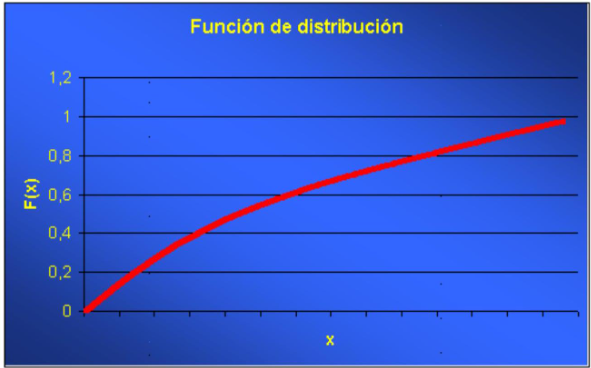
\includegraphics[width=0.9\linewidth]{images/cdfContinua}

Segundo tipo (variables discretas)

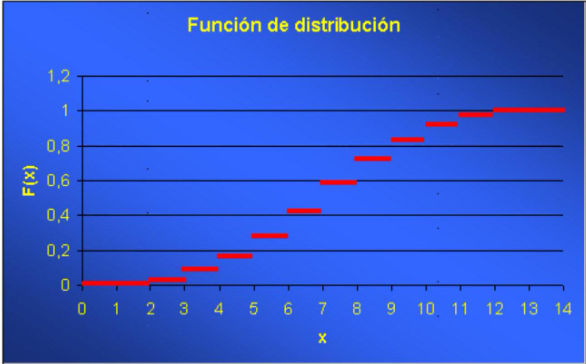
\includegraphics[width=0.9\linewidth]{images/cdfDiscreta}

\subsection{Clasificación de las variables aleatorias}\label{clasificaciuxf3n-de-las-variables-aleatorias}

Para su estudio, las variables aleatorias se clasifican en variables
discretas o variables contínuas.

\subsubsection{Variables aleatorias discretas}\label{variables-aleatorias-discretas}

\textbf{Definición: Variable aleatoria discreta}

Diremos que una variable aleatoria es discreta si su recorrido, es decir, el conjunto de valores que puede tomar, es finito
o infinito numerable.

Generalmente, este tipo de variables van asociadas
a experimentos en los cuales se cuenta el número de veces que se ha
presentado un suceso o donde el resultado es una puntuación concreta.

Los puntos del recorrido se corresponden con saltos en la gráfica de la
función de distribución, que correspondería al segundo tipo de gráfica
visto anteriormente.

\subsubsection{Variables aleatorias continuas}\label{variables-aleatorias-continuas}

\textbf{Definición: Variable aleatoria contínua}

Diremos que una variable aleatoria es continua si su función de distribución es una función
continua.

También puede definirse, de forma análoga a las variables discretas como aquellas cuyo recorrido, es decir, el conjunto de valores que puede tomar, es un intervalo o subconjunto no numerable de los números reales. En otras palabras, aquellas que pueden tomar cualquier valor dentro de un rango continuo, sin saltos entre los valores posibles.

Se corresponde con el primer tipo de gráfica visto.

Generalmente, se corresponden con variables asociadas a experimentos en
los cuales la variable medida puede tomar cualquier valor en un
intervalo; mediciones biométricas, por ejemplo.

Un caso particular dentro de las variables aleatorias continuas y al
cual pertenecen todos los ejemplos usualmente utilizados, son las
denominadas variables aleatorias absolutamente continuas.

\textbf{Definición: Distribución absolutamente contínua}

Diremos que una variable aleatoria \(X\) continua tiene una distribución
absolutamente continua si existe una función real \(f\), positiva e integrable en el conjunto de números reales, tal que la función de
distribución \(F\) de \(X\) se puede expresar como

\[
F(x)=\int_{-\infty}^{x} f(t) d t
\]

Una variable aleatoria con distribución absolutamente continua, por
extensión, se la clasifica como variable aleatoria absolutamente
continua.

\textbf{Definición: función de densidad de probabilidad}

A la función \(f\) se la denomina función de densidad de probabilidad de
la variable \(X\).

Hay que hacer notar que no toda variable continua es absolutamente
continua, pero los ejemplos son complicados, algunos utilizan para su
construcción el conjunto de Cantor, y quedan fuera del nivel y del
objetivo de este curso.

Igualmente indicaremos que los tipos de variables comentados
anteriormente forman únicamente una parte de todos los posibles tipos de
variables, sin embargo contienen prácticamente todas las variables
aleatorias que encontramos usualmente.

Tal como se estudiará más adelante, existen algunas familias de
funciones de distribución, tanto dentro del grupo de las discretas como
de las continuas, que por su importancia reciben un nombre propio y se
estudiarán en los capítulos siguientes.

En ocasiones encontramos variables de tipo mixto, es decir que se
comportan como discretas o contínuas para distintos grupos de valores.

\subsection{Variable aleatoria discretas}\label{variable-aleatoria-discretas}

Tal como se ha definido, una variable aleatoria \(X\) discreta toma valores en un conjunrto finito o numerables.

Indicaremos el recorrido de la variable \(X\) como:
\(\left\{x_{1}, x_{2}, \ldots, x_{\mathrm{k}}, \ldots\right\}\).

El ejemplo más sencillo de variable aleatoria discreta lo constituyen
las variables indicadoras. Sea \(A\) un suceso observable, se llama
indicador de \(A\) a la variable aleatoria definida por

\[
\begin{aligned}
I_{A}: \Omega & \rightarrow \mathbb{R} \\
\omega & \rightarrow I_{A}(\omega)=\left\{\begin{array}{lll}
1 & \text { si } \omega \in A \\
0 & \text { si } & A
\end{array}\right.
\end{aligned}
\]

\paragraph{Ejercicio propuesto}\label{ejercicio-propuesto}

Construir, a partir de las variables indicadoras de \(A\) y \(B\), las
siguientes variables indicadoras

\[
I_{A \cap B} ; I_{A \cup B} ; I_{A} c ; I_{\Omega}
\]

\subparagraph{Solución}\label{soluciuxf3n}

\[
\begin{gathered}
I_{A \cap B}=I_{A} \cdot I_{B} \\
I_{A \cup B}=I_{A}+I_{B}-I_{A \cap B} \\
I_{A} c=1-I_{A} \\
\Omega=1
\end{gathered}
\]

\subsubsection{Caracterización de las v.a. discretas}\label{caracterizaciuxf3n-de-las-v.a.-discretas}

Una variable aleatoria discreta puede caracterizarse a través de la
función que asocia cada elemento del recorrido su probabilidad.
Dicha función recibe varios nombres según los autores:
- función de probabilidad
- ley de probabilidad,
- función de densidad de la variable aleatoria
discreta.
- función de masa de probabilidad.

Aunque es habitual encontrar, en muchos libros el término \emph{función de densidad} para variables (absolutamente) contínuas y el término \emph{función de masa de probabilidad} para variables discretas, también lo es referirse a ambas como ``función de densidad''.

La función de probabilidad de una variable discreta se puede representar de la manera siguiente:

\[
\begin{array}{rll}
f: & \mathbb{R} & \rightarrow[0,1] \\
& x & \rightarrow f(x)=P(X=x)=P\{\omega \in \Omega \mid X(\omega)=x\}
\end{array}
\]

Obsérvese que, a diferencia de la función de distribución que toma valores para cualquier valor real, la función definida anteriormente es nula en todo punto que no
pertenezca al recorrido.

En cambio, siguiendo con la análogía, y dado que se trata de una probabilidad, la
función de densidad discreta está acotada \(0 \leq f(x) \leq 1\).

Toda
función de densidad discreta puede expresarse de manera explícita a
través de una tabla que asocie directamente puntos del recorrido con sus
probabilidades.

\textbf{Ejemplo: Función de densidad de una variable indicadora}

Consideremos la variable indicadora del suceso \(A\) :

\[
\begin{aligned}
I_{A}: \Omega & \rightarrow \mathbb{R} \\
\omega & \rightarrow I_{A}(\omega)=\left\{\begin{array}{lll}
1 & \text { si } & \omega \in A \\
0 & \text { si } & A
\end{array}\right.
\end{aligned}
\]

La función de densidad de esta variable sería la siguiente:

\begin{longtable}[]{@{}ccc@{}}
\toprule\noalign{}
\(x\) & 0 & 1 \\
\midrule\noalign{}
\endhead
\bottomrule\noalign{}
\endlastfoot
\(f(x)=P(X=x)\) & \(1-P(A)=P\left(A^{\mathrm{c}}\right)\) & \(P(A)\) \\
\end{longtable}

El recorrido está formado por dos valores: 1 y 0 , con las mismas
probabilidades que las del suceso \(A\) y su complementario,
respectivamente.

En muchos casos será posible expresar la función de probabilidadmediante una fórmula
matemática que define una regla de asignación de probabilidades para los
valores del recorrido.

\textbf{Ejemplo: Un modelo matemático para la función de probabilidad}

\[
P(X=x)=0,2 \cdot 0,8^{x-1}, \quad x=1,2, \ldots
\]

es la función de densidad de una variable aleatoria discreta con
recorrido numerable.

\subsubsection{Propiedades de la función de densidad discreta}\label{propiedades-de-la-funciuxf3n-de-densidad-discreta}

\begin{enumerate}
\def\labelenumi{\arabic{enumi}.}
\tightlist
\item
\end{enumerate}

\[
0 \leq f(x) \leq 1
\]

\begin{enumerate}
\def\labelenumi{\arabic{enumi}.}
\setcounter{enumi}{1}
\tightlist
\item
  \(\sum_{i=1}^{n} f\left(x_{i}\right)=1\), si el recorrido es finito.
\item
  \(\sum_{i=1}^{\infty} f\left(x_{i}\right)=1\), si el recorrido es
  numerable.
\end{enumerate}

\subsubsection{\texorpdfstring{Relaciones entre la función de distribución y la función de densidad discreta. Probabilidad de intervalos.}{Relaciones entre la función de distribución y la función de densidad discreta.   Probabilidad de intervalos.}}\label{relaciones-entre-la-funciuxf3n-de-distribuciuxf3n-y-la-funciuxf3n-de-densidad-discreta.-probabilidad-de-intervalos.}

Existe una relación muy importante entre las funciones de distribución
\(F(x)\) y de densidad \(f(x)\) de una variable aleatoria discreta. La
función de distribución en un punto se obtiene acumulando el valor de la
función de densidad para todos los valores del recorrido menores o
iguales al punto en cuestión.

\[
F(x)=\sum_{x_{i} \leq x} f\left(x_{i}\right) \quad \text { para todo } \mathrm{x}_{\mathrm{i}} \text { perteneciente al recorrido de la variable. }
\]

En efecto, supongamos que el recorrido de una variable discreta \(X\) es
\(\left\{x_{1}, x_{2}, \ldots, x_{k}, \ldots\right\}\) y que deseamos
conocer el valor de la función de distribución en un punto \(x\) tal que
\(x_{i} \leq x<x_{i+1}\), entonces es inmediato que

\[
F(x)=P(X \leq x)=P\left(X=x_{1}\right)+P\left(X=x_{2}\right)+\ldots+P\left(X=x_{i}\right)=f\left(x_{1}\right)+f\left(x_{2}\right)+f\left(x_{3}\right)+\ldots+f\left(x_{i}\right)
\]

Por ejemplo, para una variable indicadora de un suceso \(A\), tenemos la
relación siguiente:

\begin{longtable}[]{@{}
  >{\centering\arraybackslash}p{(\columnwidth - 4\tabcolsep) * \real{0.3333}}
  >{\centering\arraybackslash}p{(\columnwidth - 4\tabcolsep) * \real{0.3333}}
  >{\centering\arraybackslash}p{(\columnwidth - 4\tabcolsep) * \real{0.3333}}@{}}
\toprule\noalign{}
\begin{minipage}[b]{\linewidth}\centering
Valor de \(\boldsymbol{x}\)
\end{minipage} & \begin{minipage}[b]{\linewidth}\centering
\(\boldsymbol{f}(\boldsymbol{x})\)
\end{minipage} & \begin{minipage}[b]{\linewidth}\centering
\(\boldsymbol{F}(\boldsymbol{x})\)
\end{minipage} \\
\midrule\noalign{}
\endhead
\bottomrule\noalign{}
\endlastfoot
\((-\infty, 0)\) & & 0 \\
0 & \(P\left(A^{c}\right)\) & \(P\left(A^{\mathrm{c}}\right)\) \\
\((0,1)\) & & \(P\left(A^{\mathrm{c}}\right)\) \\
1 & \(P(A)\) & \(P\left(A^{\mathrm{c}}\right)+P(A)=1\) \\
\((1,+\infty)\) & & 1 \\
\end{longtable}

A partir de las funciones de densidad y de distribución es posible
expresar las probabilidades para cualquier posible intervalo de valores
de la variable. Por ejemplo:

\begin{longtable}[]{@{}l@{}}
\toprule\noalign{}
Intervalo \\
\midrule\noalign{}
\endhead
\bottomrule\noalign{}
\endlastfoot
\(P(X \leq a)=F(a)\) \\
\(P(X<a)=F(a)-f(a)\) \\
\(P(X>a)=1-F(a)=1-P(X \leq a)\) \\
\(P(X \geq a)=1-F(a)+f(a)=1-P(X>a)\) \\
\(P(a<X \leq b)=F(b)-F(a)\) \\
\(P(a<X<b)=F(b)-f(b)-F(a)\) \\
\(P(a \leq X \leq b)=F(b)-F(a)+f(a)\) \\
\(P(a \leq X<b)=F(b)-f(b)-F(a)+f(a)\) \\
\end{longtable}

\subsection{Variables aleatorias continuas}\label{variables-aleatorias-continuas-1}

Una variable aleatoria \(X\) diremos que es continua si su función de
distribución es una función continua. En la práctica, se corresponden
con variables asociadas con experimentos en los cuales la variable
medida puede tomar cualquier valor en un intervalo: mediciones
biométricas, intervalos de tiempo, áreas, etc.

\textbf{Ejemplo: Variables aleatorias continuas}

\begin{itemize}
\tightlist
\item
  Resultado de un generador de números aleatorios entre 0 y 1. Es el
  ejemplo más sencillo que podemos considerar, es un caso particular
  de una familia de variables aleatorias que tienen una distribución
  uniforme en un intervalo \([a, b]\). Se corresponde con la elección al
  azar de cualquier valor entre \(a\) y \(b\).
\item
  Estatura de una persona elegida al azar en una población. El valor
  que se obtenga será una medición en cualquier unidad de longitud ( m
  , cm , etc.) dentro de unos límites condicionados por la naturaleza
  de la variable. El resultado es impredecible con antelación, pero
  existen intervalos de valores más probables que otros debido a la
  distribución de alturas en la población. Más adelante veremos que,
  generalmente, variables biométricas como la altura se adaptan un
  modelo de distribución denominado distribución Normal y representado
  por una campana de Gauss.
\end{itemize}

Dentro de las variables aleatorias continuas tenemos las variables
aleatorias absolutamente continuas.

Diremos que una variable aleatoria \(X\) continua tiene una distribución
absolutamente continua si existe una función real \(f\), positiva e
integrable en el conjunto de números reales, tal que la función de
distribución \(F\) de \(X\) se puede expresar como

\[
F(x)=\int_{-\infty}^{x} f(t) d t
\]

Una variable aleatoria con distribución absolutamente continua, por
extensión, se clasifica como variable aleatoria absolutamente continua.

En cuanto a nuestro manual, todas las variables aleatorias continuas con
las que trabajemos pertenecen al grupo de las variables absolutamente
continuas, en particular, los ejemplos y casos expuestos.

\subsubsection{Función de densidad continua}\label{funciuxf3n-de-densidad-continua}

La función que caracteriza las variables continuas es aquella función
\(f\) positiva e integrable en los reales, tal que acumulada desde
\(-\infty\) hasta un punto \(x\), nos proporciona el valor de la función de
distribución en \(x, F(\mathrm{x})\). Recibe el nombre de función de
densidad de la variable aleatoria continua.

\[
F(x)=\int_{-\infty}^{x} f(t) d t
\]

Las funciones de densidad discreta y continua tienen, por tanto, un
significado análogo, ambas son las funciones que acumuladas (en forma de
sumatorio en el caso discreto o en forma de integral en el caso
continuo) dan como resultado la función de distribución.

La diferencia entre ambas, sin embargo, es notable.

\begin{itemize}
\tightlist
\item
  La función de densidad discreta toma valores positivos únicamente en
  los puntos del recorrido y se interpreta como la probabilidad de la
  que la variable tome ese valor \(f(x)=P(X=x)\).
\item
  La función de densidad continua toma valores en el conjunto de
  números reales y no se interpreta como una probabilidad. No está
  acotada por 1, puede tomar cualquier valor positivo. Es más, en una
  variable continua se cumple que probabilidades definidas sobre
  puntos concretos siempre son nulas.
\end{itemize}

\[
P(X=x)=0 \text { para todo } x \text { real. }
\]

¿Cómo se interpreta, entonces, la función de densidad continua? Las
probabilidades son las áreas bajo la función de densidad. El área bajo
la función de densidad entre dos puntos a y b se interpreta como la
probabilidad de que la variable aleatoria tome valores comprendidos
entre \(a\) y \(b\).

Por tanto, siempre se cumple lo siguiente:

\[
\int_{-\infty}^{+\infty} f(x) d x=1
\]

La función de densidad se expresa a través de una función matemática. La
forma específica de la función matemática generalmente pasa por
considerar a la variable aleatoria como miembro de una determinada
familia de distribuciones, un determinado modelo de probabilidad. Estas
familias generalmente dependen de uno o más parámetros y serán objeto de
un estudio específico en un capítulo posterior. La atribución a una
determinada familia depende de la naturaleza de la variable en cuestión.

Podemos ver, únicamente con ánimo ilustrativo, la expresión analítica y
la gráfica para los ejemplos comentados con anterioridad:

\begin{itemize}
\tightlist
\item
  Resultado de un generador de números aleatorios entre
  \(\boldsymbol{a}\) y \(\boldsymbol{b}\). Modelo Uniforme.
  \(f(x)=\left\{\begin{array}{cc}\frac{1}{b-a} & x \in[a, b] \\ 0 & x \notin[a, b]\end{array}\right\}\)
\item
  Estatura de una persona elegida al azar en una población. Modelo
  Normal.
\end{itemize}

\[
f(x)=\frac{1}{\sqrt{2 \pi}} e^{\frac{-(x-170)^{2}}{2}}-\infty<x<\infty
\]

\subsubsection{Relaciones entre la función de distribución y la función de densidad.}\label{relaciones-entre-la-funciuxf3n-de-distribuciuxf3n-y-la-funciuxf3n-de-densidad.}

Para una variable continua, la relación entre las funciones de
distribución y de densidad viene dada directamente a través de la
definición. La función de distribución en un punto se obtiene integrando
el valor de la función de densidad desde menos infinito hasta el punto
en cuestión. Por ejemplo:

\[
F(x)=\int_{-\infty}^{x} f(t) d t
\]

\paragraph{Probabilidad de intervalos}\label{probabilidad-de-intervalos}

A partir de las funciones de densidad y de distribución, y teniendo en
cuenta que \(P(X=x)=0\) para todo \(x\) real, es posible expresar las
probabilidades para cualquier posible intervalo de valores de la
variable. Por ejemplo:

\begin{longtable}[]{@{}c@{}}
\toprule\noalign{}
Intervalo \\
\midrule\noalign{}
\endhead
\bottomrule\noalign{}
\endlastfoot
\(P(X \leq a)=P(X<a)=F(a)=\int_{-\infty}^{a} f(x) d x\) \\
\(P(X \geq a)=P(X>a)=1-F(a)=\int_{a}^{+\infty} f(x) d x\) \\
\(P(a<X \leq b)=P(a<X<b)=P(a \leq X \leq b)=P(a \leq X<b)\) \\
\(=F(b)-F(a)=\int^{b} f(x) d x\) \\
\end{longtable}

Fijémonos que la probabilidad de los intervalos se corresponde con el
área bajo la función de densidad dentro del intervalo considerado.

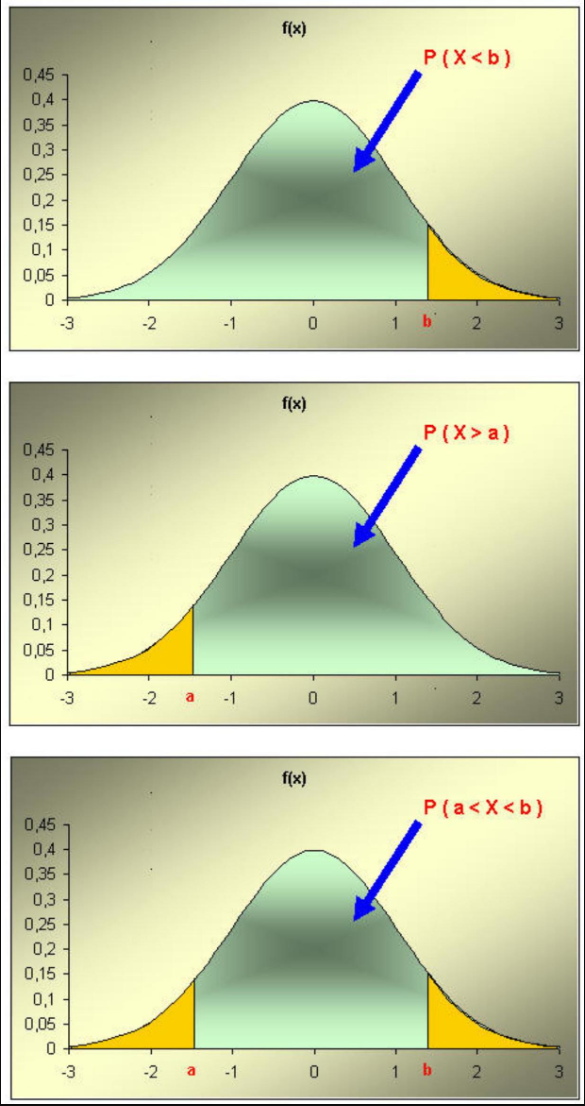
\includegraphics[width=0.8\linewidth]{images/probsDNormal}

\subsection{Caracterización de una variable aleatoria a través de parámetros}\label{caracterizaciuxf3n-de-una-variable-aleatoria-a-travuxe9s-de-paruxe1metros}

Hasta el momento hemos visto que toda variable aleatoria viene
caracterizada a través de unas determinadas funciones matemáticas, las
funciones de distribución y de densidad. Una vez caracterizada, y por
tanto conocida, la distribución de una variable aleatoria, podemos
obtener cualquier probabilidad asociada.

En ocasiones podemos acotar más el problema y reducir el estudio de una
variable aleatoria a determinar una serie de características numéricas
asociadas con la distribución de la variable. Dichas características
tienen como propiedad fundamental el hecho de resumir gran parte de las
propiedades de la variable aleatoria y juegan un papel muy destacado en
las técnicas estadísticas que desarrollaremos a lo largo del curso.

Por ejemplo, supuesta la pertenencia de una variable aleatoria a una
determinada familia de distribuciones de probabilidad, bien sea discreta
o continua, los diferentes miembros de la familia diferirán en el valor
de esas características numéricas. En este caso, denominaremos a tales
características los parámetros de la distribución.

Existe un buen número de tales características, pero nos centraremos en
las dos más importantes: la esperanza y la varianza. La primera nos
informa sobre la localización de los valores de la variable y la
segunda, sobre el grado de dispersión de estos valores.

\subsection{Esperanza de una variable aleatoria discreta}\label{esperanza-de-una-variable-aleatoria-discreta}

La esperanza matemática de una variable aleatoria es una característica
numérica que proporciona una idea de la localización de la variable
aleatoria sobre la recta real. Decimos que es un parámetro de
centralización o de localización.

Su interpretación intuitiva o significado se corresponde con el valor
medio teórico de los posibles valores que pueda tomar la variable
aleatoria, o también con el centro de gravedad de los valores de la
variable supuesto que cada valor tuviera una masa proporcional a la
función de densidad en ellos.

La definición matemática de la esperanza en el caso de las variables
aleatorias discretas se corresponde directamente con las
interpretaciones proporcionadas en el párrafo anterior. Efectivamente,
supuesta una variable aleatoria discreta \(X\) con recorrido
\(\left\{x_{1}, x_{2}, \ldots, x_{k}, \ldots\right\}\) y con función de
densidad \(f(x)\), se define la esperanza matemática de \(X\) como el valor

\[
E(X)=\sum_{x_{i} \in X(\Omega)} x_{i} f\left(x_{i}\right)
\]

donde el sumatorio se efectúa para todo valor que pertenece al recorrido
de \(X\). En caso de que el recorrido sea infinito la esperanza existe si
la serie resultante es absolutamente convergente, condición que no
siempre se cumple.

La definición se corresponde con un promedio ponderado según su
probabilidad de los valores del recorrido y, por tanto, se corresponde
con la idea de un valor medio teórico.

\subsection{Esperanza de una variable aleatoria continua}\label{esperanza-de-una-variable-aleatoria-continua}

La idea intuitiva que más nos puede ayudar en la definición de la
esperanza matemática de una variable aleatoria continua es la idea del
centro de gravedad de los valores de la variable, donde cada valor tiene
una masa proporcional a la función de densidad en ellos.

Dada una variable aleatoria absolutamente continua \(X\) con función de
densidad \(f(x)\), se define la esperanza matemática de \(X\) como el valor

\[
E(X)=\int_{-\infty}^{+\infty} x f(x) d x
\]

suponiendo que la integral exista.

\subsection{Propiedades de la esperanza matemática}\label{propiedades-de-la-esperanza-matemuxe1tica}

\begin{enumerate}
\def\labelenumi{\arabic{enumi}.}
\tightlist
\item
  Esperanza de una función de una variable aleatoria
\end{enumerate}

\begin{itemize}
\tightlist
\item
  Variable discreta
\end{itemize}

\[
E(h(X))=\sum_{x_{i} \in X(\Omega)} h\left(x_{i}\right) f\left(x_{i}\right)
\]

\begin{itemize}
\tightlist
\item
  Variable continua
\end{itemize}

\[
E(h(X))=\int_{-\infty}^{+\infty} h(x) f(x) d x
\]

\subsubsection{Linealidad de la esperanza matemática}\label{linealidad-de-la-esperanza-matemuxe1tica}

\begin{itemize}
\item
  \(E(X+Y)=E(X)+E(Y)\)
\item
  \(E(k \cdot X)=k \cdot E(X)\) para todo número real \(k\).
\item
  \(E(k)=k\) para todo número real \(k\).
\item
  \(E(a \cdot X+b)=a \cdot E(X)+b\) para todo par de números reales \(a\) y
  \(b\).
\end{itemize}

\subsubsection{Esperanza del producto}\label{esperanza-del-producto}

\begin{itemize}
\tightlist
\item
  \(E(X \cdot Y)=E(X) \cdot E(Y)\) únicamente en el caso de que \(X\) e
  \(Y\) sean variables aleatorias independientes.
\end{itemize}

\subsection{Varianza de una variable aleatoria}\label{varianza-de-una-variable-aleatoria}

La varianza de una variable aleatoria es una característica numérica que
proporciona una idea de la dispersión de la variable aleatoria respecto
de su esperanza. Decimos que es un parámetro de dispersión.

La definición es la siguiente:

\[
\operatorname{Var}(X)=E\left((X-E(X))^{2}\right)
\]

Es, por tanto, el promedio teórico de las desviaciones cuadráticas de
los diferentes valores que puede tomar la variable respecto de su valor
medio teórico o esperanza.

En el caso de las variables discretas, la expresión se convierte en:

\[
\operatorname{Var}(X)=\sum_{x_{i} \in X(\Omega)}\left(x_{i}-E(X)\right)^{2} f\left(x_{i}\right)
\]

mientras que para las variables continuas tenemos:

\[
\operatorname{Var}(X)=\int_{-\infty}^{+\infty}(x-E(X))^{2} f(x) d x
\]

En ambos casos existe una expresión equivalente alternativa y
generalmente de cálculo más fácil:

\[
\operatorname{Var}(X)=E\left(X^{2}\right)-(E(X))^{2}
\]

Una de las características de la varianza es que viene expresada en
unidades cuadráticas respecto de las unidades originales de la variable.
Un parámetro de dispersión derivado de la varianza y que tiene las
mismas unidades de la variable aleatoria es la desviación típica, que se
define como la raíz cuadrada de la varianza.

\[
\sigma_{X}=\sqrt{\operatorname{Var}(X)}=\sqrt{E\left((X-E(X))^{2}\right)}
\]

\subsubsection{Propiedades de la varianza}\label{propiedades-de-la-varianza}

\begin{enumerate}
\def\labelenumi{\arabic{enumi}.}
\tightlist
\item
  \(\operatorname{Var}(X) \geq 0\)
\item
  \(\operatorname{Var}(k \cdot X)=k^{2} \cdot \operatorname{Var}(X)\)
  para todo numero real \(k\).
\item
  \(\operatorname{Var}(k)=0\) para todo numero real \(k\).
\item
  \(\operatorname{Var}(a \cdot X+b)=a^{2} \cdot \operatorname{Var}(X)\)
  para todo par de números reales \(a\) i \(b\).
\item
  \(\operatorname{Var}(X+Y)=\operatorname{Var}(X)+\operatorname{Var}(Y)\)
  únicamente en el caso que \(X\) y \(Y\) sean independientes.
\end{enumerate}

\subsection{\texorpdfstring{Momentos (de orden \(k\)) de una variable aleatoria}{Momentos (de orden k) de una variable aleatoria}}\label{momentos-de-orden-k-de-una-variable-aleatoria}

\begin{itemize}
\tightlist
\item
  Dada una variable aleatoria \(X\), definimos el momento de orden \(k\)
  como:
\end{itemize}

\[
m_{k}=E\left(X^{k}\right)
\]

suponiendo que tal esperanza exista. Podemos ver que la esperanza es el
momento de orden \(1, E(X)=m_{1}\).

\begin{itemize}
\tightlist
\item
  Definimos el momento central de orden \(k\) como:
\end{itemize}

\[
\mu_{k}=E\left((X-E(X))^{k}\right)
\]

Con la denominación anterior, la varianza es el momento central de orden
\(2, \operatorname{Var}(X)=\mu_{2}\).

\begin{itemize}
\tightlist
\item
  Es posible también definir momentos mixtos de dos variables
  aleatorias. Dadas dos variables aleatorias \(X\) e \(Y\) definimos el
  momento mixto de orden \((r, k)\) como
\end{itemize}

\[
m_{r k}=E\left(X^{r} \cdot Y^{k}\right)
\]

y el momento mixto central de orden \((r, k)\) como

\[
\left.\mu_{r k}=E(X-E(X))^{r} \cdot(Y-E(Y))^{k}\right)
\]

\begin{itemize}
\tightlist
\item
  El momento mixto central más importante es el \(\mu_{11}\), denominado
  la covarianza de \(X\) e \(Y\), y con una interpretación en el sentido
  de cuantificar el grado de dependencia entre dos variables
  aleatorias, puesto que si \(X\) e \(Y\) son independientes se verifica
  que \(\mu_{11}=0\), mientras que si \(\mu_{11} \neq 0\) entonces las
  variables son dependientes.
\end{itemize}

\subsection{Definición formal de variable aleatoria}\label{definiciuxf3n-formal-de-variable-aleatoria}

Tal como hemos comentado, la definición formal de variable aleatoria
impone una restricción matemática en la formulación vista hasta el
momento.

Definiremos una variable aleatoria como una aplicación de \(\Omega\) en el
conjunto de números reales

\[
\begin{aligned}
X: \Omega & \rightarrow \mathbb{R} \\
\omega & \rightarrow X(\omega)
\end{aligned}
\] que verifique la propiedad siguiente

\[
\forall x \in \mathbb{R} \quad \text { el conjunto } \mathrm{A}=\{a \mid \mathrm{X}(a) \leq \mathrm{x}\} \text { es un suceso observable }
\]

es decir, para todo número real \(x\), el conjunto de resultados
elementales tales que la variable aleatoria toma sobre ellos valores
inferiores o iguales a \(x\) ha de ser un suceso sobre el cual podamos
definir una probabilidad.

Dicha propiedad recibe el nombre de medibilidad y por tanto podríamos
decir que una variable aleatoria es una función medible de \(\Omega\) en
los reales.

Esta condición nos asegura que podremos calcular sin problemas,
probabilidades sobre intervalos de la recta real a partir de las
probabilidades de los sucesos correspondientes.

\[
P(X \leq x)=P\{\omega \mid X(\omega) \leq x\}
\]

La expresión anterior se leería de la manera siguiente: La probabilidad
de que la variable aleatoria tome valores inferiores o iguales a \(x\) es
igual a la probabilidad del suceso formado por el conjunto de resultados
elementales sobre los que el valor de la variable es menor o igual que
\(x\).

La probabilidad obtenida de esta manera se denomina probabilidad
inducida. Se puede comprobar que, a partir de la condición requerida, se
pueden obtener probabilidades sobre cualquier tipo de intervalo de la
recta real. Por ejemplo:

\[
P(a<X \leq b)=P(X \leq b)-P(X \leq a)
\]

La condición exigida para ser variable aleatoria discreta ahora puede
ser expresada como:

\[
\forall k=1,2, \ldots \text { el conjunto } \mathrm{A}=\left\{\omega \mid \mathrm{X}(\omega)=\mathrm{x}_{\mathrm{k}}\right\}=\mathrm{X}^{-1}\left(\left\{\mathrm{x}_{\mathrm{k}}\right\}\right) \text { es un suceso observable }
\]

Toda variable aleatoria definida sobre un espacio de probabilidad finito
es necesariamente discreta. La suma y el producto de variables
aleatorias discretas, definido por:

\[
(X+Y)(w)=X(w)+Y(w) \text { y }(X \cdot Y)(w)=X(w) \cdot Y(w)
\]

es también una variable aleatoria discreta.

\subsection{Caso práctico: Lanzamiento de dos dados}\label{caso-pruxe1ctico-lanzamiento-de-dos-dados}

\subsubsection{Espacio muestral}\label{espacio-muestral}

Supongamos que estamos realizando un experimento consistente en el lanzamiento simultáneo de dos dados y en la observación del resultado
obtenido.

El conjunto de resultados posibles forma el espacio muestral \(\Omega\) asociado a dicho experimento. Sus elementos serán como los que se
muestran a continuación:


\includegraphics{images/clipboard-1434716414.png}

En total, el espacio muestral estaría formado por 36 resultados posibles
que, en principio y suponiendo los dados regulares, son todos ellos
equiprobables con probabilidad \(1 / 36\).

Nótese que consideramos diferentes resultados del tipo: un uno en el
primer dado y un dos en el segundo o un dos en el primer dado y un uno
en el segundo.

Una vez fijados los enunciados anteriores, es fácil asignar
probabilidades a diferentes sucesos observables, por ejemplo:

\begin{longtable}[]{@{}cc@{}}
\toprule\noalign{}
Suceso & Probabilidad \\
\midrule\noalign{}
\endhead
\bottomrule\noalign{}
\endlastfoot
Que aparezcan dos cifras iguales & \(6 \cdot 1 / 36=1 / 6\) \\
Que la suma sea 10 & \(3 \cdot 1 / 36=1 / 12\) \\
\end{longtable}

No entramos en detalles de la obtención de las probabilidades dado que
se ha estudiado suficientemente en el tema anterior.

\subsubsection{Representación numérica}\label{representaciuxf3n-numuxe9rica}

Continuando con el experimento anterior, podemos representar los
resultados obtenidos al lanzar dos dados por valores numéricos. ¿Cómo
hacerlo? Definiendo una regla de asignación numérica para cada
resultado.

Una posible regla sería, por ejemplo, asignar a cada resultado la suma
de puntos de las caras. Este enunciado nos define una variable que
representa cada suceso elemental por un valor numérico.

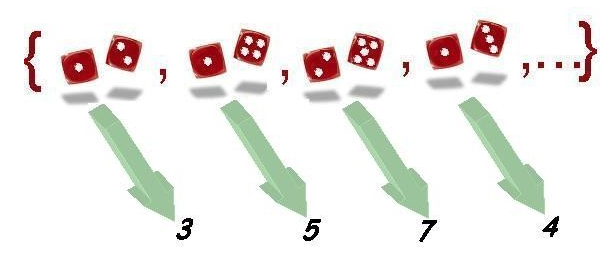
\includegraphics{images/clipboard-2572516778.png}

Los 36 posibles resultados del experimento se transforman en 11 posibles
valores numéricos para la variable: \(2,3,4,5,6,7,8,9,10,11\) y 12 .

Este conjunto de valores forman el \emph{recorrido de la variable suma de
puntos de las caras}. A partir de las probabilidades definidas sobre los
sucesos observables es fácil extender las probabilidades a los
diferentes resultados de la variable.

Por ejemplo, la probabilidad de que la variable tome el valor 10 es
equivalente a la probabilidad del suceso observable que la suma sea 10 ,
calculada anteriormente e igual a \(1 / 12\).

La variable considerada hasta el momento es sólo una de las múltiples
variables que podríamos definir sobre el mismo experimento. Por ejemplo,
podemos estar interesados no en la suma de puntos sino en el punto más
bajo de cada tirada, de forma que podríamos construir una nueva variable
a partir del enunciado o regla de asignación asignar a cada resultado el
menor de los puntos de las dos caras. Tenemos una nueva variable sobre
el mismo espacio anterior.

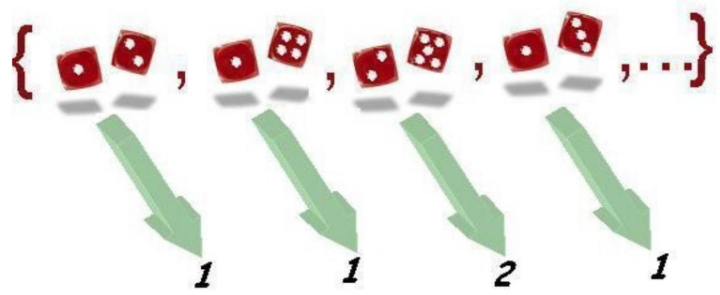
\includegraphics{images/clipboard-3898377838.png}

El recorrido, en este caso, está formado por los valores: \(1,2,3,4,5\) y
6 . Las dos variables estudiadas y otras muchas que se podrían definir
sobre este experimento son ejemplos absolutamente equivalentes desde el
punto de vista formal.

\subsubsection{Algunas probabilidades}\label{algunas-probabilidades}

En el ejemplo de los dados vamos a centrarnos en la variable aleatoria

\[
X=\text { Suma de puntos de las caras }
\]

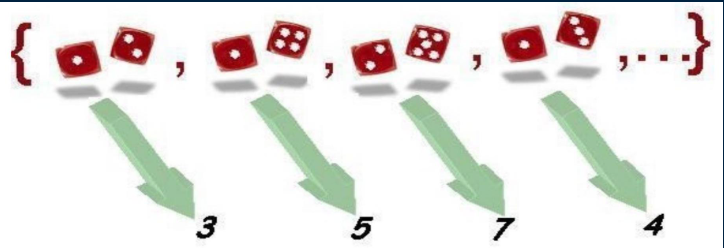
\includegraphics{images/clipboard-1018442669.png}

El recorrido de la variable está formado por los números
\(\{2,3,4,5,6,7,8,9,10,11\) i 12\(\}\). Vamos a calcular algunas
probabilidades:

\begin{itemize}
\tightlist
\item
  \(P(X \leq 1)=P\{\varnothing\}=0\) (Ningún resultado tiene asignado un
  valor menor o igual a 1)
\item
  \(P(X \leq 2)=P\{(1,1)\}=1/36\) (Sólo hay un caso al que se le asigne
  un valor inferior o igual a 2).
\item
  \(P(X \leq 3.5)=P\{(1,1), (1,2), (2,1)\}=3/36\) (Tres resultados
  elementales tienen asignado un valor menor o igual a 3.5)
\end{itemize}

Ahora podéis intentar calcular por vosotros mismos algunas
probabilidades: (a) \(P(X \leq 6)\) (b) \(P(X \leq 8,2)\); (c)
\(P(X \leq 12)\); (d) \(P(X \leq 20)\) i (e) \(P(2,2<X \leq 7)\)

\subsubsection{Función de distribución}\label{funciuxf3n-de-distribuciuxf3n}

Para calcular la función de distribución de la variable X \(=\) Suma de
puntos de las caras :

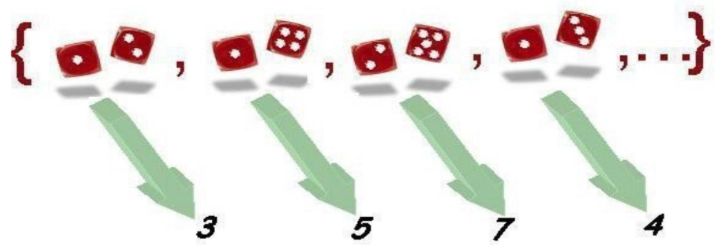
\includegraphics{images/clipboard-2353777197.png}

necesitamos conocer el recorrido de la variable, que es:
\(\{2,3,4,5,6,7,8,9,10,11, 12\}\) y, utilizando este recorrido como pauta,
determinar \emph{para todo punto} \(x\) \emph{de la recta real} la probabilidad
\(P(X \leq x)\).

En nuestro ejemplo:

\[
F(x)=P(X \leq x)= \begin{cases}0 & x<2 \\ 1 / 36 & 2 \leq x<3 \\ 3 / 36 & 3 \leq x<4 \\ 6 / 36 & 4 \leq x<5 \\ 10 / 36 & 5 \leq x<6 \\ 15 / 36 & 6 \leq x<7 \\ 21 / 36 & 7 \leq x<8 \\ 26 / 36 & 8 \leq x<9 \\ 30 / 36 & 9 \leq x<10 \\ 33 / 36 & 10 \leq x<11 \\ 35 / 36 & 11 \leq x<12 \\ 36 / 36=1 & x \geq 12\end{cases}
\]

Acabamos de construir la función de distribución de la variable suma de
la puntuación al lanzar dos dados.

Vamos a ver su representación gráfica:

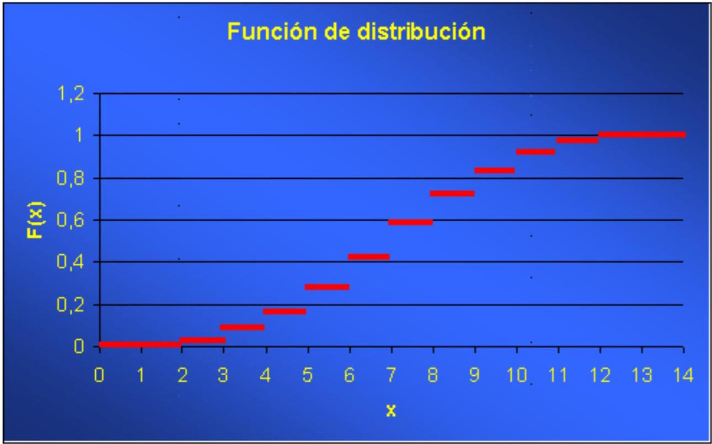
\includegraphics[width=0.9\linewidth]{images/clipboard-1894572766}

Ejercicio : Haced lo mismo para la variable aleatoria el menor de los
puntos de las dos caras al lanzar dos dados.

\subsubsection{Clasificación de las variables}\label{clasificaciuxf3n-de-las-variables}

En el experimento que estamos considerando, lanzar simultáneamente dos
dados, cualquiera de las dos variables aleatorias que hemos considerado
hasta el momento:

\[ X=\text {Suma los puntos de las dos caras } \]

\[
Y=\text { El menor de los puntos de las dos caras }
\]

se clasifican dentro del tipo de variables aleatorias discretas, puesto
que en ambos casos el recorrido es finito:
\(\{2,3,4,5,6,7,8,9,10,11, 12\}\) para la variable \(X\) y
\(\{1,2,3,4,5, 6\}\) para la variable \(Y\).

También son discretas aquellas variables aleatorias con recorrido
infinito numerable.

Ejercicio: ¿Sabríais construir una variable aleatoria discreta con
recorrido infinito numerable basada en el experimento que consiste en el
lanzamiento de dos dados?

\subsubsection{Función de densidad discreta}\label{funciuxf3n-de-densidad-discreta}

Para calcular la función de densidad de la variable

\[
X=\text { suma de puntos de las caras }
\]

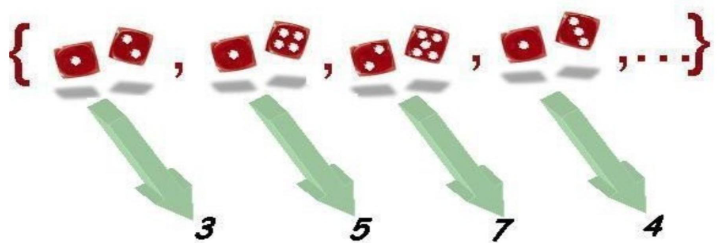
\includegraphics{images/clipboard-2707476680.png}

necesitamos conocer el recorrido de la variable, es decir:
\(\{2,3,4,5,6,7,8,9,10,11, 12\}\) y, a partir del recorrido, determinar
para todo punto del recorrido la probabilidad \(P(X=x)\).

En nuestro ejemplo

\[
f(x)=P(X=x)= \begin{cases}1 / 36 & x=2 \\ 2 / 36 & x=3 \\ 3 / 36 & x=4 \\ 4 / 36 & x=5 \\ 5 / 36 & x=6 \\ 6 / 36 & x=7 \\ 5 / 36 & x=8 \\ 4 / 36 & x=9 \\ 3 / 36 & x=10 \\ 2 / 36 & x=11 \\ 1 / 36 & x=12\end{cases}
\]

Acabamos de construir la función de densidad de la variable suma de la
puntuación al lanzar dos dados.

Vamos a ver su representación gráfica:

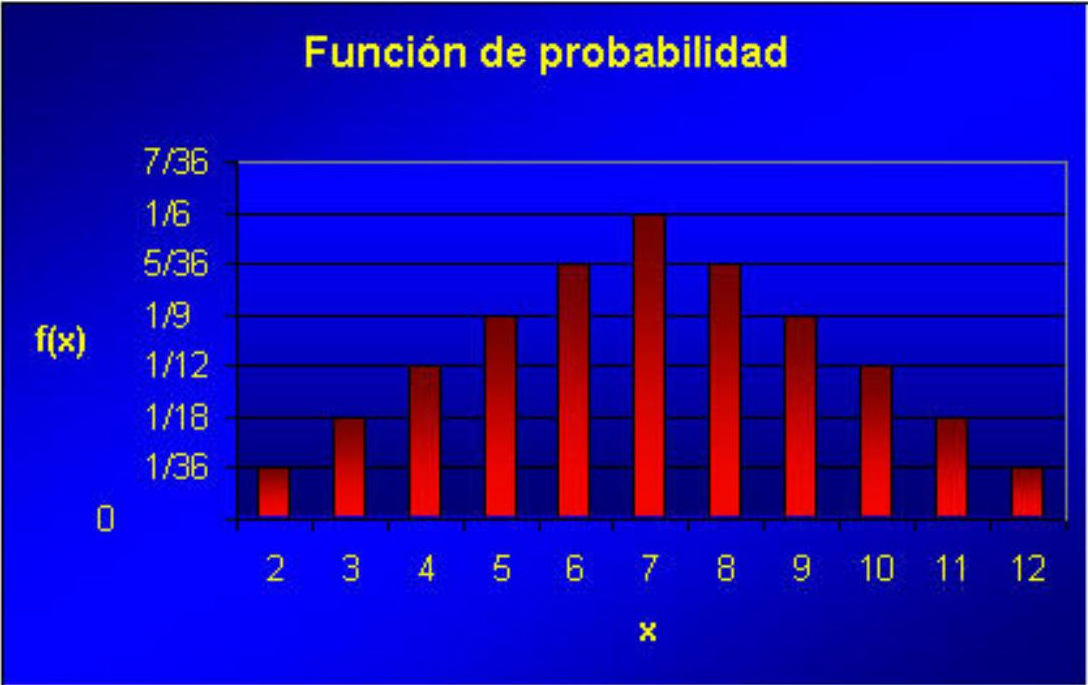
\includegraphics[width=0.8\linewidth]{images/fmp2Dados}

Hemos optado por la representación con barras en lugar de puntos para
permitir una visualización de la función óptima.

Ejercicio: Haced lo mismo para la variable aleatoria el menor de los
puntos de las dos caras al lanzar dos dados.

\subsubsection{Probabilidad de intervalos}\label{probabilidad-de-intervalos-1}

Vamos a centrarnos en la variable

\[
X=\text { Suma de puntos de las caras }
\]

Las funciones de distribución y de densidad son, respectivamente,

\[
F(x)=P(X \leq x)=\left\{\begin{array}{ll}
0 & x<2 \\
1 / 36 & 2 \leq x<3 \\
3 / 36 & 3 \leq x<4 \\
6 / 36 & 4 \leq x<5 \\
10 / 36 & 5 \leq x<6 \\
15 / 36 & 6 \leq x<7 \\
21 / 36 & 7 \leq x<8 \\
26 / 36 & 8 \leq x<9 \\
30 / 36 & 9 \leq x<10 \\
33 / 36 & 10 \leq x<11 \\
35 / 36 & 11 \leq x<12 \\
36 / 36=1 & x \geq 12
\end{array} \quad f(x)=P(X=x)= \begin{cases}1 / 36 & x=2 \\
2 / 36 & x=3 \\
3 / 36 & x=4 \\
4 / 36 & x=5 \\
5 / 36 & x=6 \\
6 / 36 & x=7 \\
5 / 36 & x=8 \\
4 / 36 & x=9 \\
3 / 36 & x=10 \\
2 / 36 & x=11 \\
1 / 36 & x=12\end{cases}\right.
\]

Puede observarse cómo los valores de la función de distribución se
obtienen acumulando los valores de la función de densidad
correspondientes.

Vamos a calcular algunas probabilidades utilizando las funciones
anteriores. Compárese con los resultados obtenidos con anterioridad
basados directamente en los resultados elementales.

\begin{itemize}
\tightlist
\item
  \(P(X \leq 1)=F(1)=0\)
\item
  \(P(X \leq 3,5)=F(3,5)=3 / 36=f(2)+f(3)\)
\item
  \(P(X<6)=F(6)-f(6)=15 / 36-5 / 36=10 / 36=f(2)+f(3)+f(4)+f(5)\)
\item
  \(P(2,2<X \leq 7)=F(7)-F(2,2)=21 / 36-1 / 36=20 / 36=f(3)+f(4)+f(5)+f(6)+f(7)\)
\item
  \(P(2<X<7)=F(7)-f(7)-F(2)=21 / 36-6 / 36-1 / 36=14 / 36=f(3)+f(4)+f(5)+f(6)\)
\end{itemize}

\subsubsection{Esperanza}\label{esperanza}

Supongamos que estamos interesados en determinar cual sería el valor
medio teórico de la variable

\[
X=\text { Suma de puntos de las caras }
\]

La función de densidad es:

\[
f(x)=P(X=x)= \begin{cases}1 / 36 & x=2 \\ 2 / 36 & x=3 \\ 3 / 36 & x=4 \\ 4 / 36 & x=5 \\ 5 / 36 & x=6 \\ 6 / 36 & x=7 \\ 5 / 36 & x=8 \\ 4 / 36 & x=9 \\ 3 / 36 & x=10 \\ 2 / 36 & x=11 \\ 1 / 36 & x=12\end{cases}
\]

La misma función de densidad nos da información sobre el recorrido de la
variable. Calcular el valor medio teórico de la variable quiere decir
calcular la esperanza. A partir de la fórmula de la esperanza para
variables discretas, tenemos

\[
\begin{aligned}
E(X) &=2 \cdot 1 / 36+3 \cdot 2 / 36+4 \cdot 3 / 36+5 \cdot 4 / 36+6 \cdot 5 / 36+\\
& + 7 \cdot 6 / 36+8 \cdot 5 / 36+9 \cdot 4 / 36+\\
&+ 10 \cdot 3 / 36+ 
11 \cdot 2 / 36+12 \cdot 1 / 36=\\
& =7
\end{aligned}
\]

Por tanto, 7 es la esperanza de la variable \(X=\) Suma de puntos de las
caras. Fijaos que la esperanza para la variable Puntuación de un dado
sería

\[
1 \cdot 1 / 6+2 \cdot 1 / 6+3 \cdot 1 / 6+4 \cdot 1 / 6+5 \cdot 1 / 6+6 \cdot 1 / 6=3,5
\]

y que se puede considerar la variable Suma de puntos de las dos caras
como la suma de dos variables que representen la puntuación de cada
dado. La esperanza de la suma es, efectivamente, la suma de las
esperanzas de cada variable sumada.

En la aplicación siguiente, podéis calcular la esperanza de la variable
Puntuación de un dado y modificar las probabilidades de las diferentes
caras, de este modo se modifica la esperanza.

Ejercicio: ¿Podríais hacer lo mismo para la variable \(X=\) El menor de
los puntos de las dos caras al lanzar dos dados?

\subsubsection{Esperanza de un juego}\label{esperanza-de-un-juego}

Imaginemos que alguien os propone el juego siguiente: lanzad dos dados,
si la suma obtenida es menor o igual a 6 ganáis 100 euros, sin embargo,
si la suma obtenida es mayor que 6 tenéis que pagar 100 euros. ¿Nos
conviene jugar a este juego?

Veamos, podemos considerar el resultado del juego como una variable
aleatoria discreta que toma dos valores: +100 si ganamos y -100 si
perdemos. Nos interesa conocer las probabilidades de los diferentes
resultados. Consideremos la variable \(X=\) Suma de puntos de las caras,
cuya función de densidad conocemos:

\[
f(x)=P(X=x)= \begin{cases}1 / 36 & x=2 \\ 2 / 36 & x=3 \\ 3 / 36 & x=4 \\ 4 / 36 & x=5 \\ 5 / 36 & x=6 \\ 6 / 36 & x=7 \\ 5 / 36 & x=8 \\ 4 / 36 & x=9 \\ 3 / 36 & x=10 \\ 2 / 36 & x=11 \\ 1 / 36 & x=12\end{cases}
\]

A partir de aquí es fácil ver que la función de densidad de la variable
\(Y=\) Resultado del juego será la siguiente:

\[
f(100)=15 / 36 ; f(-100)=21 / 36
\]

Por tanto, la esperanza del juego, que puede ser interpretada como la
ganancia media por jugada, será

\[
E(Y)=100 \cdot 15 / 36-100 \cdot 21 / 36=-100 / 6 \approx-16,667
\]

Es decir, la ganancia media por jugada es negativa, por tanto no es
favorable dicho juego para el jugador, es un juego no equitativo.

\subsubsection{Esperanza con recorrido infinito}\label{esperanza-con-recorrido-infinito}

Vamos a tratar de calcular la esperanza de la siguiente variable
aleatoria: \(X=\) Número de lanzamientos que hemos de hacer para conseguir
que aparezca un doble seis La variable que acabamos de definir es una
variable discreta con recorrido infinito numerable. El recorrido sería
el siguiente:

\[
\{1,2,3,4, \ldots\}
\]

Vamos a ver como calculamos la función de densidad: \(P(X=1)=\)
Probabilidad de que aparezca un doble seis en el primer lanzamiento
\(=1 / 36\) \(P(X=2)=\) Probabilidad de que el doble seis no aparezca en el
primer lanzamiento y sí en el segundo =
\(35 / 36 \cdot 1 / 36=35 / 36^{2}\) \(P(X=3)=\) Probabilidad de que el
doble seis no aparezca ni en el primer ni en el segundo lanzamientos y
sí en el tercero \(=35 / 36 \cdot 35 / 361 / 36=35^{2} / 36^{3}\)

En general, \(P(X=k)=35^{k-1} / 36^{k}\) Para simplificar, vamos a llamar
\(p=1 / 36\) y \(q=1-p=35 / 36\), con esta nomenclatura
\(P(X=\mathrm{k})=q^{k-1} p\). Por tanto, la esperanza será:

\[
\begin{aligned}
E(X)& =\sum_{i=1}^{\infty} i q^{i-1} p=p \sum_{i=1}^{\infty} i q^{i-1}=p \frac{d}{d q} \sum_{i=1}^{\infty} q^{i}= \\ 
&= p \frac{d}{d q}\left(\frac{q}{1-q}\right)=p \frac{1}{(1-q)^{2}}=\\
& = \frac{1}{p}
\end{aligned}
\]

En nuestro ejemplo el número medio de tiradas antes de salir un doble
seis será 36 .

\subsubsection{Esperanza infinita}\label{esperanza-infinita}

Ahora calcularemos la esperanza del juego siguiente: lanzamos un dado
hasta que aparece un número par, el jugador gana \(2^{n}\) unidades
monetarias si aparece un número par por primera vez en la tirada nésima.

El recorrido de la variable aleatoria \(X=\) Ganancia del juego, está
formado por todos los números de la forma \(2^{n}\) con \(n=1,2,3, \ldots\)
La probabilidad de cada valor del recorrido es la probabilidad de que
aparezca un número par por primera vez en la tirada nésima, es decir
\((1 / 2)^{n-1} \cdot(1 / 2)=(1 / 2)^{n}\). Por tanto, la esperanza del
juego es la siguiente:

\[
E(X)=\sum_{n=1}^{\infty} 2^{n}(1 / 2)^{n}=\sum_{n=1}^{\infty} 1=\infty
\]

Como vemos, la variable aleatoria \(X\) no tiene esperanza finita. El
enunciado presentado es una versión del problema presentado alrededor de
1730 por el matemático Daniel Bernouilli a la Academia de San
Petersburgo y conocido como la paradoja de San Petersburgo, dado que la
esperanza del juego es aparentemente infinita.

\subsubsection{Varianza}\label{varianza}

Si ahora queremos calcular la varianza de la variable

\[
X=\text { Suma de puntos de las caras }
\]

con función de densidad:

\[
f(x)=P(X=x)= \begin{cases}1 / 36 & x=2 \\ 2 / 36 & x=3 \\ 3 / 36 & x=4 \\ 4 / 36 & x=5 \\ 5 / 36 & x=6 \\ 6 / 36 & x=7 \\ 5 / 36 & x=8 \\ 4 / 36 & x=9 \\ 3 / 36 & x=10 \\ 2 / 36 & x=11 \\ 1 / 36 & x=12\end{cases}
\]

Podemos aplicar la fórmula

\[
\operatorname{Var}(X)=E\left(X^{2}\right)-(E(X))^{2}
\]

La esperanza ya la tenemos calculada con anterioridad

\[
\begin{aligned}
E(X) & =2 \cdot 1 / 36+3 \cdot 2 / 36+4 \cdot 3 / 36+5 \cdot 4 / 36+\\
& +6 \cdot 5 / 36+7 \cdot 6 / 36+8 \cdot 5 / 36+9 \cdot 4 / 36+\\
& +10 \cdot 3 / 36+ 11 \cdot 2 / 36+12 \cdot 1 / 36=\\
& =7
\end{aligned}
\]

Necesitamos calcular la esperanza de la variable al cuadrado, que en
este caso resulta:

\[
\begin{aligned}
E\left(X^{2}\right)& =2^{2} \cdot 1 / 36+3^{2} \cdot 2 / 36+4^{2} \cdot 3 / 36+5^{2} \cdot 4 / 36+6^{2} \cdot 5 / 36+\\
& + 7^{2} \cdot 6 / 36+8^{2} \cdot 5 / 36+9^{2} \cdot 4 / 36+  10^{2} \cdot 3 / 36+\\
& + 11^{2} \cdot 2 / 36+12^{2} \cdot 1 / 36=329 / 6 \\
&\approx 54,833
\end{aligned}
\]

Con lo que la varianza resulta ser

\[
\operatorname{Var}(X)=329 / 6-7^{2}=35 / 6 \approx 5,833
\]

Nuevamente, para la variable Puntuación de un dado, la varianza se
obtendría de la manera siguiente:

\[
\begin{aligned}
E(X)& =1 \cdot 1 / 6+2 \cdot 1 / 6+3 \cdot 1 / 6+4 \cdot 1 / 6+5 \cdot 1 / 6+6 \cdot 1 / 6= \\& =3,5\\
E \left(X^{2}\right)&=1^{2} \cdot 1 / 6+2^{2} \cdot 1 / 6+3^{2} \cdot 1 / 6+4^{2} \cdot 1 / 6+\\
& + 5^{2} \cdot 1 / 6+6^{2} \cdot 1 / 6=91 / 6\\ &  \approx 15,167 \\
\operatorname{Var}(X)&=91 / 6-3,5^{2}=35 / 12 \approx 2,9167
\end{aligned}
\]

y se cumple que la varianza de la variable Suma de puntos de las dos
caras es la suma de las varianzas de las puntuaciones de cada dado por separado. Recordemos que esto sólo sucede si las variables sumadas son independientes, como así ocurre con las puntuaciones de cada dado por separado.

\section{Distribuciones Notables}\label{distribuciones-notables}

\subsection{Distribuciones discretas}\label{distribuciones-discretas}

\subsubsection{La distribución de Bernouilli}\label{la-distribuciuxf3n-de-bernouilli}

Es el modelo discreto más sencillo en que podamos pensar. Hace referencia a situaciones en las que el resultado de un experimento sólo puede ser: se ha dado el suceso \(A\) ó no se ha dado el suceso \(A\). Por ejemplo, en el lanzamiento de una moneda sólo puede darse el suceso sale cara o su complementario no sale cara (sale cruz).

Por lo tanto, definimos la variable aleatoria \(X\) de la siguiente manera:

\begin{itemize}
\tightlist
\item
  \(X=1\) si se ha dado \(A\).
\item
  \(X=0\) si no se ha dado \(A\), es decir, se ha dado el complementario \(A^{c}\).
\end{itemize}

Si además, conocemos la probabilidad de que suceda \(A\) :

\[
P[A]=p
\]

y, por tanto,

\[
P\left[A^{c}\right]=1-p
\]

ya podemos definir la distribución de la variable aleatoria \(X\).
En estas condiciones diremos que \(X\) sigue una distribución de Bernouilli de parámetro \(p\), que abreviaremos así \(X \sim \operatorname{Bernouilli}(p)\), y su función de densidad se define así:

\[
f(k)=P[X=k]=\left\{\begin{array}{cc}
p & \text { si } k=1(\text { se ha dado } A) \\
1-p & \text { si } k=0\left(\text { se ha dado } A^{c}\right)
\end{array}\right\}
\]

Gráficamente:

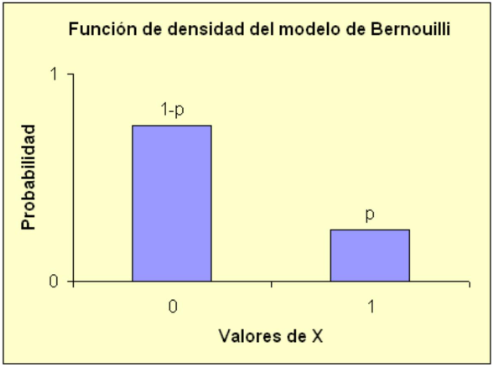
\includegraphics[width=0.8\linewidth]{images/fmpBernouilli}

Mientras que la función de distribución será:

\[
F(k)=P[X \leq k]=\left\{\begin{array}{lc}
0 & \text { si } \mathbf{k}<0 \\
\mathbf{p} & \text { si } 0 \leq \mathbf{k}<1 \\
1 & \text { si } \mathbf{p} \geq 1
\end{array}\right\}
\]

Gráficamente:

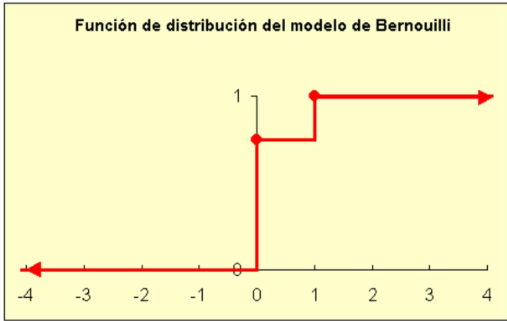
\includegraphics[width=0.8\linewidth]{images/cdfBernouilli}

\paragraph{Propiedades del modelo de Bernouilli}\label{propiedades-del-modelo-de-bernouilli}

\begin{enumerate}
\def\labelenumi{\arabic{enumi})}
\tightlist
\item
  La esperanza vale \(E(X)=p\).
\item
  La varianza vale \(V(X)=p(1-p)\).
\end{enumerate}

\subsubsection{La distribución Binomial}\label{la-distribuciuxf3n-binomial}

Al igual que el modelo de Bernouilli, hace referencia a experiencias con resultados dicotómicos (el resultado sólo puede ser \(A\) o \(A^{\mathcal{C}}\) ). Sin embargo en este modelo estamos interesados en la repetición de \(n\) veces una experiencia de este tipo en condiciones independientes.

Tomemos el ejemplo del contaje del número de caras en el lanzamiento \(n\) veces de una moneda regular.
Para concretar, vamos a suponer que disponemos de una moneda regular \((P[\) cara \(]=P[c r u z]=1 / 2)\) que lanzamos cuatro veces. Es evidente que, en estas condiciones, la variable X: número de caras en cuatro lanzamientos independientes de una moneda regular es una variable aleatoria discreta que sólo puede tomar cinco posibles valores:

\[
x=0,1,2,3,4
\]

Pasemos ahora a calcular la probabilidad de cada valor (en terminología estadística, vamos a calcular la función de densidad de la variable \(X\) ).

Es evidente que la \(P[X=0]\) es igual a la probabilidad de salgan cuatro cruces seguidas:

\[
P[X=0]=P[c r u z, c r u z, c r u z, c r u z]=\mathrm{P}[c r u z]^{4}=(1 / 2)^{4}=0,0625
\]

ya que la moneda es regular y, por tanto, \(P[\) cara \(]=P[\) cruz \(]=1 / 2\).
La \(P[X=3]\) corresponde al suceso de que salgan tres caras ( \(c\) en adelante) y una cruz ( + en adelante). Sin embargo, en este caso tenemos hasta cuatro posibles maneras de obtener dicho resultado, según el orden en que aparezcan las tres caras y la cruz:

\begin{longtable}[]{@{}
  >{\centering\arraybackslash}p{(\columnwidth - 6\tabcolsep) * \real{0.2500}}
  >{\centering\arraybackslash}p{(\columnwidth - 6\tabcolsep) * \real{0.2500}}
  >{\centering\arraybackslash}p{(\columnwidth - 6\tabcolsep) * \real{0.2500}}
  >{\centering\arraybackslash}p{(\columnwidth - 6\tabcolsep) * \real{0.2500}}@{}}
\toprule\noalign{}
\begin{minipage}[b]{\linewidth}\centering
+ccc
\end{minipage} & \begin{minipage}[b]{\linewidth}\centering
\(\mathrm{c}+\mathrm{cc}\)
\end{minipage} & \begin{minipage}[b]{\linewidth}\centering
\(\mathrm{cc}+\mathrm{c}\)
\end{minipage} & \begin{minipage}[b]{\linewidth}\centering
\(\mathrm{ccc}+\)
\end{minipage} \\
\midrule\noalign{}
\endhead
\bottomrule\noalign{}
\endlastfoot
\end{longtable}

También debería resultar evidente que la probabilidad de cada uno de estos sucesos es la misma:

\[
P[+\mathrm{ccc}]=P[\mathrm{c}+\mathrm{cc}]=P[\mathrm{cc}+\mathrm{c}]=P[\mathrm{ccc}+]=(1 / 2)^{4}=(1 / 2)^{4}=0,0625
\]

de manera que, finalmente, la probabilidad de que salgan tres caras y una cruz es la suma de las probabilidades de los 4 casos anteriores:

\[
P[X=3]=4(1 / 2)^{4}=0,25
\]

Y así podríamos ir calculando el resto de casos. Podemos ver que, en este ejemplo, todos los casos tienen la misma probabilidad \((0,0625)\) y que el número total de casos posibles es 16 . En términos de combinatoria dicho número se obtendría como variaciones con repetición de dos valores (cara o cruz) tomados de cuatro en cuatro (el número de lanzamientos de la moneda):

\[
V R_{2}{ }^{4}=2^{4}=16
\]

En la siguiente tabla se muestran los dieciséis posibles resultados:

\begin{longtable}[]{@{}cc@{}}
\toprule\noalign{}
\(k=\) número de caras & Casos \\
\midrule\noalign{}
\endhead
\bottomrule\noalign{}
\endlastfoot
0 & +++++ \\
1 & +++c \\
& \(++\mathrm{c}+\) \\
& \(+\mathrm{c}++\) \\
& \(\mathrm{c}+++\) \\
& ++cc \\
& \(+\mathrm{c}+\mathrm{c}\) \\
& \(\mathrm{c}++\mathrm{c}+\) \\
& \(\mathrm{c}+\mathrm{c}+\) \\
& cc++ \\
& \(\mathrm{ccc}+\) \\
& \(\mathrm{c}+\mathrm{cc}\) \\
\end{longtable}

Si hacemos uso de nuestros conocimientos de combinatoria, comprobamos que el número de casos para cada posible valor \(k(k=0,1,2,3,4)\) puede calcularse como permutaciones con repetición de cuatro elementos tomado de \(k\) y \(4-k\) :

\[
R P_{4}^{k, 4-k}=\frac{4!}{k!(4-k)!}=\binom{4}{k}
\]

y obtenemos finalmente el número combinatorio 4 sobre \(k\). En efecto, para el caso \(k=3\), tendríamos:

\[
\binom{4}{3}=\frac{4!}{3!1!}=4
\]

que son los cuatro posibles casos que nos dan tres caras y una cruz.
Finalmente, recordando que todos los casos tienen la misma probabilidad, se construye la siguiente tabla:

\begin{longtable}[]{@{}ccc@{}}
\toprule\noalign{}
\(k=\) número de caras & Número de casos & \(P[X=k]\) \\
\midrule\noalign{}
\endhead
\bottomrule\noalign{}
\endlastfoot
0 & 1 & 0,0625 \\
1 & 4 & 0,2500 \\
& & \\
\end{longtable}

\begin{longtable}[]{@{}ccc@{}}
\toprule\noalign{}
2 & 6 & 0,3750 \\
\midrule\noalign{}
\endhead
\bottomrule\noalign{}
\endlastfoot
3 & 4 & 0,2500 \\
4 & 1 & 0,0625 \\
Total & 16 & 1 \\
\end{longtable}

\paragraph{Los parámetros de la distribución Binomial}\label{los-paruxe1metros-de-la-distribuciuxf3n-binomial}

La última tabla de la página anterior es, justamente, la función de densidad de nuestra variable \(X\).

\begin{longtable}[]{@{}cc@{}}
\toprule\noalign{}
Función de densidad de \(X\) & \\
\midrule\noalign{}
\endhead
\bottomrule\noalign{}
\endlastfoot
\(k\) & \(P[X=k]\) \\
0 & 0,0625 \\
1 & 0,2500 \\
2 & 0,3750 \\
3 & 0,2500 \\
4 & 0,0625 \\
En otro caso & 0 \\
\end{longtable}

Como hemos visto, para obtener los resultados anteriores, hemos tenido que definir dos valores:

\begin{enumerate}
\def\labelenumi{\arabic{enumi}.}
\tightlist
\item
  \(n\) : el número de lanzamientos (repeticiones de la experiencia aleatoria en condiciones independientes), en nuestro caso \(n=4\).
\item
  \(p\) : la probabilidad de que salga cara \((P[c])\), en nuestro caso \(p=1 / 2\).
\end{enumerate}

Se dice, por tanto, que la distribución Binomial depende de dos parámetros: \(n\) y \(p\). En nuestro ejemplo, diremos que \(X\) sigue una distribución Binomial de parámetros \(n=4\) i \(p=1 / 2\). De forma abreviada:

\[
X \sim B(n=4 ; p=1 / 2)
\]

En el ejemplo que hemos visto, suponíamos que la moneda era regular y, por tanto,

\[
P[c]=P[+]=1 / 2
\]

Si tenemos una moneda trucada con las siguientes probabilidades:

\[
P[c]=2 / 3 \quad \text { i } \quad P[+]=1 / 3
\]

diremos que en este caso la variable \(X\) : número de caras en cuatro lanzamientos independientes de nuestra moneda trucada sigue una distribución Binomial de parámetros:

\[
X \sim B(n=4 ; p=2 / 3)
\]

El problema se nos complica levemente ya que ahora no todos los posibles resultados tienen la misma probabilidad. Veamos dos ejemplos:

\begin{itemize}
\tightlist
\item
  La probabilidad de obtener cuatro caras es:
\end{itemize}

\[
P[c c c c]=(2 / 3)^{4}=0,1975
\]

\begin{itemize}
\tightlist
\item
  La probabilidad de que el primer lanzamiento sea cara y el resto sean cruces valdrá:
\end{itemize}

\[
P\left[c^{+++}\right]=(2 / 3)^{\prime}(1 / 3)^{3}=0,0247
\]

Sin embargo sí se cumplirá que la probabilidad de que todos los caso que resulten en el mismo número de caras y cruces tendrán la misma probabilidad. Por ejemplo, para los cuatro casos en los que el número total de caras es 1 y el de cruces 3 :

\[
P[c+++]=P[+c++]=P[++c+]=P[+++c]=(2 / 3)^{\prime}(1 / 3)^{3}=0,0247
\]

Y, por tanto, la probabilidad de obtener una sola cara en el lanzamiento de nuestra moneda trucada será:

\[
P[X=1]=4^{\prime} 0,0247=0,0988
\]

O, generalizando, si \(P[A]=p\) y \(P\left[A^{c}\right]=1-p\) tenemos que

\[
P[X=k]=c(n, k) p^{k}(1-\mathrm{p})^{n-k} \quad \text { si } k=0,1, \ldots, n
\]

donde \(c(n, k)\) representa el número de posibles resultados en los que obtenemos \(k\) caras y \(n-k\) cruces en \(n\) lanzamientos. Tal como hemos visto, dicho número se puede calcular como permutaciones con repetición de \(n\) unidades tomadas de \(k\) y \(n-k\).

Todo lo anterior nos lleva a formular el model binoial a traves de la siguiente función de densidad:

\[
f(k)=P[X=k]=\left\{\begin{array}{ll}
\binom{\mathbf{n}}{\mathbf{k}} p^{k}(1-p)^{n-k} & \text { si } \quad k=0, \ldots, n \\
0 & \text { en caso contrario }
\end{array}\right\}
\]

con lo que la función de distribución se calcularía:

\[
F(k)=P[X \leq k]=\left\{\begin{array}{cc}
0 & \text { si } k<0 \\
\sum_{i=0}^{k}\binom{\mathbf{i}}{\mathbf{n}} p^{i}(\mathbf{1}-p)^{n-i} \\
\mathbf{1} & \text { si } k \geq n
\end{array}\right\}
\]

\paragraph{Propiedades del modelo Binomial}\label{propiedades-del-modelo-binomial}

\begin{enumerate}
\def\labelenumi{\arabic{enumi}.}
\tightlist
\item
  La esperanza vale \(E(X)=n p\).
\item
  La varianza es \(V(X)=n p(1-p)\).
\item
  Es una generalización del modelo de Bernouilli. En efecto, la Binomial con \(n=1\) (una sola realización) coincide con la distribución de Bernouilli.
\item
  La suma de dos variables aleatorias binomiales independientes con igual parámetro \(p\) también sigue una distribución Binomial:
\end{enumerate}

\[
X_{1} \sim B\left(n=n_{1} ; p=p_{0}\right) \quad \text { i } \quad X_{2} \sim B\left(n=n_{2} ; p=p_{0}\right)
\]

Si definimos \(Z=X_{1}+X_{2}\) entonces,

\[
Z \sim B\left(n=n_{1}+n_{2} ; p=p_{0}\right)
\]

\subsubsection{La distribución de Poisson}\label{la-distribuciuxf3n-de-poisson}

Se trata de un modelo discreto, pero en el que el conjunto de valores con probabilidad no nula no es finito, sino numerable. Se dice que una variable aleatoria \(X\) sigue la distribución de Poisson si su función de densidad viene dada por:

\[
f(k)=P[X=k]=\left\{\begin{array}{ll}
e^{-\lambda \frac{\lambda^{k}}{k!}} & \text { si } k=0,12, \ldots \\
0 & \text { en caso contrario }
\end{array}\right\}
\]

Como vemos, este modelo se caracteriza por un sólo parámetro \(\lambda\), que debe ser positivo.
Esta distribución suele utilizarse para contajes del tipo número de individuos por unidad de tiempo, de espacio, etc.

\paragraph{Propiedades del modelo de Poisson}\label{propiedades-del-modelo-de-poisson}

\begin{enumerate}
\def\labelenumi{\arabic{enumi}.}
\tightlist
\item
  Esperanza: \(E(X)=\lambda\).
\item
  Varianza: \(V(X)=\lambda\).
\end{enumerate}

En esta distribución la esperanza y la varianza coinciden.

\begin{enumerate}
\def\labelenumi{\arabic{enumi}.}
\setcounter{enumi}{2}
\tightlist
\item
  La suma de dos variables aleatorias independientes con distribución de Poisson resulta en una nueva variable aleatoria, también con distribución de Poisson, de parámetro igual a la suma de parámetros:
\end{enumerate}

\[
X_{1} \sim P\left(\lambda=\lambda_{1}\right) \quad \text { y } \quad X_{2} \sim P\left(\lambda=\lambda_{2}\right)
\]

y definimos \(Z=X_{1}+X_{2}\), entonces,

\[
Z \sim P\left(\lambda=\lambda_{1}+\lambda_{2}\right)
\]

Este resultado se extiende inmediatamente al caso de \(n\) variables aleatorias independientes con distribución de Poisson. En este caso, la variable suma de todas ellas sigue una distribución de Poisson de parámetro igual a la suma de los parámetros.

\subsubsection{La distribución Uniforme discreta}\label{la-distribuciuxf3n-uniforme-discreta}

Tenemos esta distribución cuando el resultado de una experiencia aleatoria puede ser un conjunto finito de \(n\) posibles resultados, todos ellos igualmente probables.

Un ejemplo puede ser la variable \(X\), puntuación en el lanzamiento de un dado regular. Esta variable toma seis valores posibles, todos con la misma probabilidad \(p=1 / 6\). La función de densidad de esta variable será:

\[
f(k)=P[X=k]=1 / 6 \quad k=1,2,3,4,5,6
\]

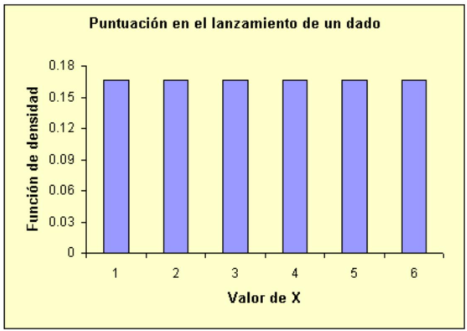
\includegraphics[width=0.8\linewidth]{images/pmfUnifDiscreta}

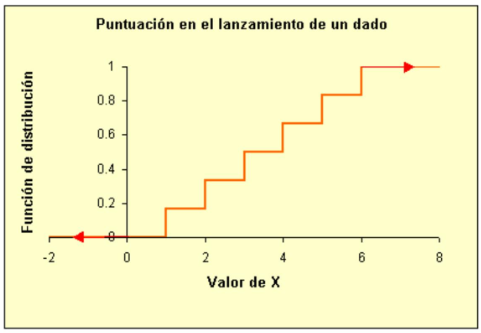
\includegraphics[width=0.8\linewidth]{images/cdfUnifDiscreta}

En general, si la variable \(X\) puede tomar \(n(k=1,2, \ldots, n)\) valores, todos con igual probabilidad, su función de densidad será:

\[
f(k)=P[X=k]=1 / n \quad k=1,2, \ldots, n
\]

\paragraph{Propiedades del modelo Uniforme discreto}\label{propiedades-del-modelo-uniforme-discreto}

Sea \(n\) el número de valores equiprobables posibles:

\paragraph{Esperanza:}\label{esperanza-1}

\[
E(X)=\frac{n+1}{2}
\]

\paragraph{Varianza:}\label{varianza-1}

\[
V(X)=\frac{(n+1)[2(2 n+1)-3(n+1)]}{12}
\]

\subsubsection{La distribución Hipergeométrica}\label{la-distribuciuxf3n-hipergeomuxe9trica}

Este modelo presenta similitudes con el Binomial, pero sin la suposición de independencia de éste último. Veámoslo:

\begin{itemize}
\tightlist
\item
  Partimos de un conjunto formado por \(N\) individuos divididos en dos categorías mutuamente excluyentes: \(A\) y \(A^{c}\); de manera que \(N_{1}\) individuos pertenecen a la categoría \(A\) y \(N_{2}\) individuos, a la categoría \(A^{c}\). Por tanto, se cumple que
\end{itemize}

\[
N=N_{1}+N_{2}
\]

\begin{itemize}
\tightlist
\item
  Si del conjunto anterior extraemos \(n\) individuos sin reemplazamiento \((n \leq N)\), la variable \(X\) que representa el número k de individuos que pertenecen a la categoría A (de los n extraídos) tiene por función de densidad:
\end{itemize}

\[
f(k)=P[X=k]=\frac{\binom{\mathbf{N}_{1}}{\mathbf{k}}\binom{\mathrm{N}_{2}}{\mathbf{n}-\mathbf{k}}}{\binom{\mathbf{N}}{\mathbf{n}}}
\]

si \(\operatorname{max}\left\{0, \mathrm{n}-N_{2}\right\} \leq \mathrm{k} \leq \min \left\{N_{1}, n\right\}\)

La dependencia se debe al hecho de que \(N\) es finito y las extracciones se efectúan sin reemplazamiento. El caso de extracciones con reemplazamiento sería equivalente al de \(N\) infinito y se resolvería mediante el modelo Binomial.

\paragraph{Propiedades del modelo hipergeométrico}\label{propiedades-del-modelo-hipergeomuxe9trico}

\begin{enumerate}
\def\labelenumi{\arabic{enumi}.}
\item
  Esperanza: \(\mathrm{E}(\mathrm{X})=\mathrm{n} \mathrm{N}_{1} / \mathrm{N}_{2}\).
\item
  Varianza: \(V(X)=\left(n N_{1} N_{2}(N-n)\right) /\left(N_{2}(N-1)\right)\)
\end{enumerate}

\subsubsection{La distribución Geométrica o de Pascal}\label{la-distribuciuxf3n-geomuxe9trica-o-de-pascal}

Definamos una experiencia aleatoria cuyo resultado sólo puede ser el suceso \(A\) o su complementario \(A^{c}\), y que se repite secuencialmente hasta que aparece el suceso \(A\) por primera vez.

Definamos la variable aleatoria \(X\) como el número de veces que repetimos la experiencia en condiciones independientes hasta que se dé A por primera vez. Bajo estas condiciones, decimos que la variable \(X\) sigue una distribución geométrica o de Pascal de parámetro \(p=P(A)\).

La función de densidad puede deducirse fácilmente de la definición:

\[
f(k)=P[X=k]=(1-p)^{k} p \quad k=0,1,2, \ldots
\]

En el programa siguiente podéis ver su forma y obtener los valores de la función de densidad y de la de distribución:

Algunas puntualizaciones de la definición de \(X\) :

\begin{itemize}
\tightlist
\item
  Notése que, en esta definición, condiciones independientes significa que \(p\), la probabilidad de \(A\), y \(1-p\), la de su complementario \(A^{c}\), no varían a lo largo de las sucesivas repeticiones de la experiencia.
\item
  Tal y como la hemos definido, \(X\) se refiere al número de lanzamientos hasta que se produce \(A\), pero sin contabilizar el último caso en que se da \(A\). Por dicha razón \(X\) puede tomar los valores \(k=\) \(0,1,2, \ldots\) con probabilidad no nula.
\end{itemize}

Un ejemplo de este modelo podría ser la experiencia consistente en lanzar sucesivamente un dado regular hasta que aparezca el número 6 . Si definimos la variable aleatoria \(X\) como el número de lanzamientos de un dado regular hasta que aparezca un 6 , queda claro que \(X\) sigue una distribución geométrica de parámetro \(p=1 / 6\).

\paragraph{Propiedades del modelo Geométrico o de Pascal}\label{propiedades-del-modelo-geomuxe9trico-o-de-pascal}

\begin{enumerate}
\def\labelenumi{\arabic{enumi})}
\tightlist
\item
  Esperanza: \(E(X)=(1-p) / p\)
\item
  Varianza: \(V(X)=(1-p) / p^{2}\)
\end{enumerate}

\paragraph{Preguntas:}\label{preguntas}

\begin{itemize}
\item
  ¿A que suceso nos referimos cuando decimos \(X=0\) ? Respuesta.

  \begin{itemize}
  \tightlist
  \item
    Cuando decimos que \(X=0\) nos referimos al caso en que el 6 aparece en el primer lanzamiento. La probabilidad de que esto suceda, suponiendo un dado regular, es de \(1 / 6\) :
  \end{itemize}
\end{itemize}

\[
P[X=0]=1 / 6
\]

\begin{itemize}
\item
  ¿Cuál es la probabilidad de que el primer 6 aparezca en el cuarto lanzamiento? Respuesta.

  \begin{itemize}
  \tightlist
  \item
    La probabilidad de que el primer 6 aparezca en el cuarto lanzamiento corresponde a:
  \end{itemize}
\end{itemize}

\[
P[X=3]=(5 / 6)^{3 \cdot} 1 / 6=0,0965
\]

Fijémonos en que, si definimos \(A\) como el suceso sale un 6, la probabilidad anterior corresponde a la del suceso: \(\left\{A^{c} A^{c} A^{c} A\right\}\) (en este orden).

\subsubsection{La distribución Binomial negativa}\label{la-distribuciuxf3n-binomial-negativa}

Puede definirse como una generalización del modelo Geométrico o de Pascal. Así, dado un suceso \(A\) y su complementario \(A^{c}\), cuando \(X\) representa el número de veces que se da \(\mathrm{A}^{\mathrm{c}}\) (ausencias, fallos, etc.) hasta que se produce r veces el suceso A , en una serie de repeticiones de la experiencia aleatoria en condiciones independientes, decimos que \(X\) sigue la distribución Binomial negativa. Nótese que, cuando \(r=1\), tenemos exactamente el modelo geométrico.

Este modelo queda definido por dos parámetros \(p\) (la probabilidad de \(A: p=P(A)\) ) y \(r\) (el número de veces que debe producirse \(A\) para que detengamos la experiencia).

La función de densidad viene dada por:

\[
f(k)=P[X=k]=\binom{\mathbf{k}+\mathbf{r}-\mathbf{1}}{\mathbf{r}-\mathbf{1}} \mathbf{p}^{\mathbf{r}} \mathbf{q}^{\mathbf{k}} \quad \mathbf{k}=\mathbf{0}, \mathbf{1}, \mathbf{2}, \ldots
\]

donde \(q\) representa el complementario de \(p: q=1-p\).

\paragraph{Propiedades del modelo Binomial negativo}\label{propiedades-del-modelo-binomial-negativo}

\begin{enumerate}
\def\labelenumi{\arabic{enumi}.}
\item
  Esperanza: \(E(X)=r^{\prime} q / p\)
\item
  Varianza: \(V(X)=r^{\prime} q / p^{2}\)
\item
  Se cumplen las siguientes propiedades respecto la función de densidad:
\end{enumerate}

\[
f(0)=p^{r} \quad \text { y } \quad f(k+1)=\frac{(1-p)(k+r)}{k+1} f(k)
\]

\begin{enumerate}
\def\labelenumi{\arabic{enumi}.}
\setcounter{enumi}{3}
\item
  Este modelo se ajusta bien a contajes (números de individuos por unidad de superficie) cuando se produce una distribución contagiosa (los individuos tienden a agruparse).
\item
  La distribución Binomial negativa puede definirse con mayor generalidad si tomamos \(r\) como un número real positivo cualquiera (no necesariamente entero). Pero, en dicho caso, se pierde el carácter intuitivo del modelo y se complican ligeramente los cálculos. Por dichas razones, se ha excluido dicha posibilidad en esta presentación.
\end{enumerate}

\subsubsection{Tabla resumen de las distribuciones discretas principales}\label{tabla-resumen-de-las-distribuciones-discretas-principales}

\begin{longtable}[]{@{}
  >{\centering\arraybackslash}p{(\columnwidth - 8\tabcolsep) * \real{0.2000}}
  >{\centering\arraybackslash}p{(\columnwidth - 8\tabcolsep) * \real{0.2000}}
  >{\centering\arraybackslash}p{(\columnwidth - 8\tabcolsep) * \real{0.2000}}
  >{\centering\arraybackslash}p{(\columnwidth - 8\tabcolsep) * \real{0.2000}}
  >{\centering\arraybackslash}p{(\columnwidth - 8\tabcolsep) * \real{0.2000}}@{}}
\toprule\noalign{}
\begin{minipage}[b]{\linewidth}\centering
Distribución
\end{minipage} & \begin{minipage}[b]{\linewidth}\centering
Parámetros
\end{minipage} & \begin{minipage}[b]{\linewidth}\centering
Función de densidad
\end{minipage} & \begin{minipage}[b]{\linewidth}\centering
Esperanza
\end{minipage} & \begin{minipage}[b]{\linewidth}\centering
Varianza
\end{minipage} \\
\midrule\noalign{}
\endhead
\bottomrule\noalign{}
\endlastfoot
Bernouilli & \(0 \leq p \leq 1\) & \(p^{k}(1-p)^{1-k}\) \(k=0,1\) & \(p\) & \(p(1-p)\) \\
Binomial & \(0 \leq p \leq 1\) \(n=1,2, \ldots\) & \(\binom{\mathbf{n}}{\mathbf{k}} p^{k}(1-p)^{n-k}\) \(k=0,1, \ldots, n\) & \(n p\) & \(n p(1-p)\) \\
Poisson & \(\lambda>0\) & \(e^{-\lambda} \frac{\lambda^{k}}{k!}\) \(k=012, \ldots\) & \(\lambda\) & \(\lambda\) \\
Multinomial & \(0 \leq p_{1}, \ldots\) \(p_{r} \leq 1\) \(\left(p_{1}+\ldots+\right.\) \(\left.p_{\mathrm{r}}=1\right)\) \(n=1,2\) & \(\frac{n!}{k_{1}!k_{2}!\cdots k_{r}!} p_{1}^{k_{1}} p_{2}^{k_{2}} \cdots p_{r}^{k_{r}}\) \(\sum_{i=1}^{r} k_{i}=n\) & \(\left(\begin{array}{c}n p_{1} \\ n p_{2} \\ \vdots \\ n p_{r}\end{array}\right)\) & \(\boldsymbol{\sigma}_{i i}=n p_{i}\left(1-p_{i}\right)\) \(\boldsymbol{\sigma}_{i j}=n p_{i} p_{j} \quad i \neq j\) \\
Uniforme discreta & \(n=1,2, \ldots\) & \(\frac{1}{n}\) \(k=1,2, \ldots . n\) & \(\frac{n+1}{2}\) & \(\frac{(n+1)[2(2 n+1)-3(n+1)}{12}\) \\
Hipergeométrica & \(\left\{\begin{array}{c}N=N_{1}+ \\ N_{2} \\ p=N_{1} / N\end{array}\right.\) & \(\frac{\binom{\mathrm{N}_{1}}{\mathrm{k}}\binom{\mathrm{N}_{2}}{\mathrm{n}-\mathrm{k}}}{\binom{\mathrm{N}}{\mathrm{n}}}\) \(\operatorname{max}\left\{0, \mathrm{n}-N_{2}\right\} \leq \mathrm{k} \leq \min \left\{N_{1}, n\right\}\) & \(n p\) & \(n p(1-p) \frac{N-n}{N-1}\) \\
Pascal & \(0 \leq p \leq 1\) & \(p(1-p)^{k}\) \(k=0,1,2, \ldots\) & \(\frac{1-p}{p}\) & \(\frac{1-p}{p^{2}}\) \\
Binomial negativa & \(0 \leq p \leq 1\) \(r>0\) & & \(\frac{r(1-p)}{p}\) & \(\frac{r(1-p)}{p^{2}}\) \\
\end{longtable}

\subsection{Distribuciones Continuas}\label{distribuciones-continuas}

\subsubsection{La distribución Uniforme}\label{la-distribuciuxf3n-uniforme}

La distribución Uniforme es el modelo (absolutamente) continuo más simple. Corresponde al caso de una variable aleatoria que sólo puede tomar valores comprendidos entre dos extremos \(a\) y \(b\), de manera que todos los intervalos de una misma longitud (dentro de \((a, b)\) ) tienen la misma probabilidad. También puede expresarse como el modelo probabilístico correspondiente a tomar un número al azar dentro de un intervalo \((a, b)\).

De la anterior definición se desprende que la función de densidad debe tomar el mismo valor para todos los puntos dentro del intervalo \((a, b)\) (y cero fuera del intervalo). Es decir,

\[
f_{X}(x)=\left\{\begin{array}{ll}
\frac{1}{b-a} & \text { si } x \in(a, b) \\
0 & \text { si } x \notin(a, b)
\end{array}\right\}
\]

Gráficamente:

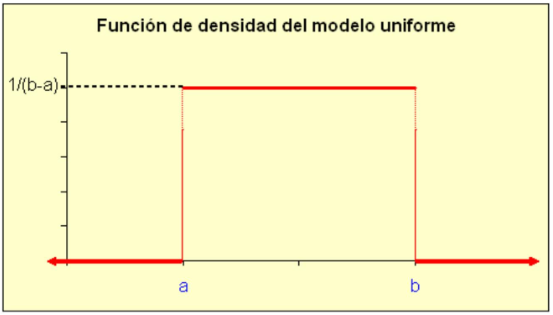
\includegraphics[width=0.8\linewidth]{images/pdfUnifContinua}

La función de distribución se obtiene integrando la función de densidad y viene dada por:

\[
F_{X}(x)=P(X \leq x)=\left\{\begin{array}{ll}
0 & \text { si } x \leq a \\
\frac{x-a}{b-a} & \text { si } x \in(a, b) \\
1 & \text { si } x \geq b
\end{array}\right\}
\]

Gráficamente:

Función de distribución del modelo uniforme

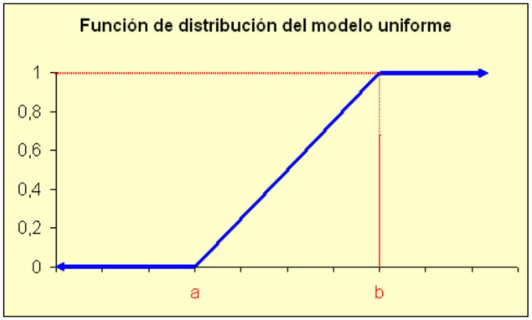
\includegraphics[width=0.8\linewidth]{images/cdfUnifContinua}

\paragraph{Propiedades del modelo Uniforme}\label{propiedades-del-modelo-uniforme}

\begin{enumerate}
\def\labelenumi{\arabic{enumi}.}
\tightlist
\item
  Su esperanza vale \((b+a) / 2\)
\item
  Su varianza es \((b-a)^{2} / 12\)
\end{enumerate}

\paragraph{Una aplicación del modelo Uniforme: el muestreo de Montecarlo}\label{una-aplicaciuxf3n-del-modelo-uniforme-el-muestreo-de-montecarlo}

En ciertos casos es útil simular el muestreo de una variable aleatoria con una distribución dada. El muestreo de Montecarlo es un procedimiento general para obtener muestras aleatorias de cualquier tipo de variable (discreta o continua) si su función de distribución es conocida o se puede calcular.

Supongamos que queremos generar una muestra procedente de una variable aleatoria \(X\) con función de distribución \(F(x)\). El proceso comprende los siguientes pasos:

\begin{enumerate}
\def\labelenumi{\arabic{enumi}.}
\item
  Obtener un valor aleatorio \(y\) entre cero y uno. Es decir, obtener una muestra de una distribución Uniforme entre cero y uno. La mayoría de lenguajes de programación incorporan un generador de este tipo.
\item
  Considerar el valor obtenido como el valor de la función de distribución a generar: \(y=F(x)\).
\item
  El valor \(x=F^{-1}(y)\) (la inversa de la función de distribución en el punto \(y\) ) es un valor procedente de la distribución de la que deseábamos generar la muestra.
\item
  Si queremos obtener una muestra con \(n\) individuos debemos repetir los pasos anteriores \(n\) veces.
\end{enumerate}

\paragraph{Generación de una muestra procedente de una distribución Binomial}\label{generaciuxf3n-de-una-muestra-procedente-de-una-distribuciuxf3n-binomial}

Supongamos que queremos simular el experimento de contar el número de caras obtenidas en 5 lanzamientos de una moneda trucada con probabilidad de cara igual a 0,75 . Es decir, queremos obtener una muestra de una distribución Binomial con \(n=5\) y \(p=0,75\).

Siguiendo los pasos anteriores deberemos obtener un número al azar entre 0 y 1 (un valor procedente de una distribución Uniforme entre 0 y 1) y si este valor es menor o igual a 0,75 diremos que ha salido cara y, si es superior a 0,75 , cruz. Utiliza el siguiente programa para simular cinco lanzamientos con nuestra moneda trucada:

\subsubsection{La distribución Exponencial}\label{la-distribuciuxf3n-exponencial}

Este modelo suele utilizarse para variables que describen el tiempo hasta que se produce un determinado suceso.

Su función de densidad es de la forma:

\[
f(x)=\left\{\begin{array}{lll}
\frac{1}{\alpha} \exp \left(-\frac{x}{\alpha}\right) & \text { si } & x>0 \\
0 & \text { si } & x \leq 0
\end{array}\right\}
\]

Como vemos este modelo depende de un único parámetro \(\alpha\) que debe ser positivo: \(\alpha>0\). A continuación se muestra un programa que nos permite ver cómo cambia la forma de la función de densidad según el parámetro \(\alpha\).

La función de distribución se obtiene integrando la de densidad y es de la forma:

\[
F(x)=\left\{\begin{array}{lll}
1-\exp \left(-\frac{x}{\alpha}\right) & \text { si } & x>0 \\
0 & \text { si } & x \leq 0
\end{array}\right\}
\]

Podemos utilizar el programa siguiente para calcular dicha función de distribución:

\paragraph{Propiedades del modelo Exponencial}\label{propiedades-del-modelo-exponencial}

\begin{enumerate}
\def\labelenumi{\arabic{enumi}.}
\item
  Su esperanza es \(\alpha\).
\item
  Su varianza es \(\alpha^{2}\).
\item
  Una propiedad importante es la denominada \emph{carencia de memoria}, que podemos definir así: si la variable \(X\) mide el tiempo de vida y sigue una distribución Exponencial, significará que la probabilidad de que siga con vida dentro de 20 años es la misma para un individuo que a fecha de hoy tiene 25 años que para otro que tenga 60 años.
\item
  Cuando el número de sucesos por unidad de tiempo sigue una distribución de Poisson de parámetro \(\lambda\) (proceso de Poisson), el tiempo entre dos sucesos consecutivos sigue una distribución Exponencial de parámetro \(\alpha=1 / \lambda\).
\end{enumerate}

\subsubsection{La distribución Normal}\label{la-distribuciuxf3n-normal}

Se trata, sin duda, del modelo continuo más importante en estadística, tanto por su aplicación directa, veremos que muchas variables de interés general pueden describirse por dicho modelo, como por sus propiedades, que han permitido el desarrollo de numerosas técnicas de inferencia estadística. En realidad, el nombre de Normal proviene del hecho de que durante un tiempo se creyó, por parte de médicos y biólogos, que todas las variables naturales de interés seguían este modelo.

Su función de densidad viene dada por la fórmula:

\[
f(x)=\frac{1}{\sqrt{2 \pi} \sigma} \exp \left\{-\frac{(x-\mu)^{2}}{2 \sigma^{2}}\right\} \quad \text { donde }-\infty<x<+\infty
\]

que, como vemos, depende de dos parámetros \(\mu\) (que puede ser cualquier valor real) y \(\sigma\) (que ha de ser positiva). Por esta razón, a partir de ahora indicaremos de forma abreviada que una variable \(X\) sigue el modelo Normal así: \(X \sim N(\mu, \sigma)\). Por ejemplo, si nos referimos a una distribución Normal con \(\mu=0\) y \(\sigma\) \(=1\) lo abreviaremos \(N(0,1)\).

A continuación vemos gráfica de esta función de densidad (podeis probar a cambiar los parámetros):

Como puedes ver, la función de densidad del modelo Normal tiene forma de campana, la que habitualmente se denomina campana de Gauss. De hecho, a este modelo, también se le conoce con el nombre de distribución gaussiana.

\paragraph{Propiedades del modelo Normal}\label{propiedades-del-modelo-normal}

\begin{enumerate}
\def\labelenumi{\arabic{enumi}.}
\item
  Su esperanza es \(\mu\).
\item
  Su varianza es \(\sigma^{2} \mathrm{y}\), por tanto, su desviación típica es \(\sigma\).
\item
  Es simétrica respecto a su media \(\mu\), como puede apreciarse en la representación anterior.
\item
  Media, moda y mediana coinciden \((\mu)\).
\item
  Cualquier transformación lineal de una variable con distribución Normal seguirá también el modelo Normal. Si \(X \sim N(\mu, \sigma)\) y definimos \(Y=a X+b(\operatorname{con} a \neq 0)\), entonces \(Y \sim N(a \mu+b,|a| \sigma)\). Es decir, la esperanza de \(Y\) será \(a \mu+b\) y su desviación típica, \(|a| \sigma\).
\item
  Cualquier combinación lineal de variables normales independientes sigue también una distribución Normal. Es decir, dadas \(n\) variables aleatorias independientes con distribución \(X_{i} \sim\) \(N\left(\mu_{i}, \sigma_{i}\right)\) para \(i=1,2, \ldots, n\) la combinación lineal: \(Y=a_{n} X_{n}+a_{n-1} X_{n-1}+\ldots+a_{1} X_{1}+\mathrm{a}_{0}\) sigue también el modelo Normal:
\end{enumerate}

\[
Y \approx N\left(a_{0}+\sum_{i=1}^{n} a_{i} \boldsymbol{\mu}_{i}, \sqrt{\sum_{i=1}^{n} a_{i}^{2} \boldsymbol{\sigma}^{2}}\right)
\]

\#\#\#La función de distribución del modelo Normal

La función de distribución del modelo Normal se debería calcular, como en el resto de distribuciones continuas, integrando la función de densidad:

\[
F(x)=P[X \leq x]=\int_{-\infty}^{x} \frac{1}{\sqrt{2 \pi} \sigma} \exp \left\{-\frac{(t-\mu)^{2}}{2 \sigma^{2}}\right\} \mathrm{dt}
\]

Pero nos encontramos con el problema de que no existe ninguna primitiva conocida para esta función, es decir, no sabemos resolver la anterior integral. Sin embargo, si somos incapaces de calcular la función distribución no podremos efectuar ningún cálculo con este modelo. ¿Cómo solucionamos el problema?

Una primera solución podría consistir en aproximar la integral a través de técnicas de cálculo numérico. Sin embargo, dado que el conjunto de valores que pueden tomar los parámetros \(\mu\) y \(\sigma\) son infinitos, deberíamos repetir el proceso para cada valor diferente de algún parámetro. Afortunadamente, podemos ahorrarnos el esfuerzo aprovechando la propiedad de que cualquier transformación lineal de una variable Normal sigue también el modelo Normal. Por tanto, replantearemos cualquier problema en términos de una Normal concreta, que suele ser la \(\mathrm{N}(0,1)\), de la siguiente manera:

Si \(X \sim N(\mu, \sigma)\) y entonces definimos \(Z=(\mathrm{X}-\mu) / \sigma\) se cumplirá que \(Z \sim N(0,1)\)

\[
\begin{gathered}
\text { y, por tanto: } \\
F_{X}(x)=P[X \leq x]=P\left[\frac{X-\boldsymbol{\mu}}{\boldsymbol{\sigma}} \leq \frac{x-\boldsymbol{\mu}}{\boldsymbol{\sigma}}\right]=P\left[Z \leq \frac{x-\boldsymbol{\mu}}{\boldsymbol{\sigma}}\right]=F_{Z}\left(\frac{x-\boldsymbol{\mu}}{\boldsymbol{\sigma}}\right)
\end{gathered}
\]

A la distribución \(N(0,1)\), es decir, la que tiene por media cero y por desviación típica uno, se le denomina Normal reducida o tipificada. En cambio, al proceso de transformación del cálculo de la función de distribución de una Normal cualquiera a través de la Normal tipificada, se le denomina tipificación.

Debemos remarcar que el proceso de tipificación no resuelve el problema de la inexistencia de la función primitiva correspondiente. Sin embargo, sí es posible, mediante técnicas de cálculo numérico, obtener la integral numérica correspondiente y elaborar unas tablas que podemos consultar. Naturalmente, la tipificación permite que con una sola tabla, la de la \(N(0,1)\), tengamos suficiente.

Hoy en día, cada vez se utilizan menos tablas como la mencionada anteriormente, ya que los ordenadores, junto con los abundantes programas estadísticos existentes nos resuelven este problema. Sin embargo, la imposibilidad de integrar analíticamente la función de densidad persiste y, aunque nosotros no seamos conscientes, los programas informáticos realizan el proceso de tipificación para simplificar el problema.

\subsubsection{La distribución Gamma}\label{la-distribuciuxf3n-gamma}

Este modelo es una generalización del modelo Exponencial ya que, en ocasiones, se utiliza para modelar variables que describen el tiempo hasta que se produce p veces un determinado suceso.

Su función de densidad es de la forma:

\[
f(x)=\left\{\begin{array}{lll}
\frac{1}{\alpha^{p} \Gamma(p)} e^{-\frac{x}{\alpha}} x^{p-1} & \text { si } & x>0 \\
0 & \text { si } & x \leq 0
\end{array}\right\}
\]

Como vemos, este modelo depende de dos parámetros positivos: \(\alpha\) y p.~La función \(\Gamma(p)\) es la denominada función Gamma de Euler que representa la siguiente integral:

\[
\Gamma(p)=\int_{0}^{\infty} x^{p-1} e^{-x} d x
\]

que verifica \(\Gamma(p+1)=p \Gamma(p)\), con lo que, si \(p\) es un número entero positivo, \(\Gamma(p+1)=p\).

\paragraph{Propiedades de la distribución Gamma}\label{propiedades-de-la-distribuciuxf3n-gamma}

\begin{enumerate}
\def\labelenumi{\arabic{enumi}.}
\item
  Su esperanza es \(p \alpha\).
\item
  Su varianza es \(p \alpha^{2}\)
\item
  La distribución Gamma \((\alpha, p=1)\) es una distribución Exponencial de parámetro \(\alpha\). Es decir, el modelo Exponencial es un caso particular de la Gamma \(\operatorname{con} p=1\).
\item
  Dadas dos variables aleatorias con distribución Gamma y parámetro \(\alpha\) común
\end{enumerate}

\[
X \sim G\left(\alpha, p_{1}\right) \text { y } Y \sim G\left(\alpha, p_{2}\right)
\]

se cumplirá que la suma también sigue una distribución Gamma

\[
X+Y \sim G\left(\alpha, p_{1}+p_{2}\right)
\]

Una consecuencia inmediata de esta propiedad es que, si tenemos \(k\) variables aleatorias con distribución Exponencial de parámetro \(\alpha\) (común) e independientes, la suma de todas ellas seguirá una distribución \(G(\alpha, k)\).

\subsubsection{La distribución de Cauchy}\label{la-distribuciuxf3n-de-cauchy}

Se trata de un modelo continuo cuya función de densidad es:

\[
f(x)=\frac{1}{\pi\left(1+x^{2}\right)} \quad \text { para } \quad-\infty<x<\infty
\]

Cuya integral nos proporciona la función de distribución:

\[
F(x)=\int_{-\infty}^{x} \frac{1}{\pi\left(1+t^{2}\right)} d t=\frac{1}{\pi}[\arctan (t)]_{t=-\infty}^{t=x}=\frac{1}{2}+\frac{\arctan (x)}{\pi}
\]

El siguiente programa permite visualizar la forma de la función de densidad de este modelo y el valor de la función de distribución:

\paragraph{Propiedades de la distribución de Cauchy}\label{propiedades-de-la-distribuciuxf3n-de-cauchy}

Se trata de un ejemplo de variable aleatoria que carece de esperanza (y, por tanto, también de varianza o cualquier otro momento), ya que la integral impropia correspondiente no es convergente:

\[
E(X)=\int_{-\infty}^{\infty} \frac{x}{\pi\left(1+x^{2}\right)} d x=\frac{1}{2 \pi} \int_{-\infty}^{\infty} \frac{2 x}{1+x^{2}} d x=\frac{1}{2 \pi}\left[\lim _{x \rightarrow \infty} \ln \left(x^{2}\right)-\lim _{x \rightarrow-\infty} \ln \left(x^{2}\right)\right]=\frac{1}{2 \pi}[\infty-\infty]
\]

y nos queda una indeterminación. Por tanto, la esperanza de una distribución de Cauchy no existe. Cabe señalar que la función de densidad es simétrica respecto al valor cero (que sería la mediana y la moda), pero al no existir la integral anterior, la esperanza no existe.

\subsubsection{La distribución de Weibull}\label{la-distribuciuxf3n-de-weibull}

Se trata de un modelo continuo asociado a variables del tipo tiempo de vida, tiempo hasta que un mecanismo falla, etc. La función de densidad de este modelo viene dada por:

\[
f(x)=\left\{\begin{array}{ll}
\frac{\beta}{\alpha}\left(\frac{x}{\alpha}\right)^{\beta-1} e^{-\left(\frac{x}{\alpha}\right)^{\beta}} & \text { si } x \geq 0 \\
0 & \text { si } x<0
\end{array}\right\}
\]

que, como vemos, depende de dos parámetros: \(\alpha>0\) y \(\beta>0\), donde \(\alpha\) es un parámetro de escala y \(\beta\) es un parámetro de forma (lo que proporciona una gran flexibilidad a este modelo).

La función de distribución se obtiene por la integración de la función de densidad y vale:

\[
F(x)=1-e^{-\left(\frac{x}{\alpha}\right)^{\beta}}
\]

El siguiente programa permite visualizar la forma de la función de densidad de este modelo y el valor de la función de distribución:

\paragraph{Propiedades de la distribución Weibull}\label{propiedades-de-la-distribuciuxf3n-weibull}

\begin{enumerate}
\def\labelenumi{\arabic{enumi}.}
\item
  Si tomamos \(\beta=1\) tenemos una distribución Exponencial.
\item
  Su esperanza vale:
\end{enumerate}

\[
E(X)=\alpha \Gamma\left(\frac{1}{\boldsymbol{\beta}}+\mathbf{1}\right)
\]

\begin{enumerate}
\def\labelenumi{\arabic{enumi}.}
\setcounter{enumi}{2}
\tightlist
\item
  Su varianza vale:
\end{enumerate}

\[
V(X)=\alpha^{2}\left\{\Gamma\left(\frac{2}{\beta}+1\right)-\left[\Gamma\left(\frac{1}{\beta}+1\right)\right]^{2}\right\}
\]

donde \(\Gamma(x)\) representa la función Gamma de Euler definida anteriormente.

\subsubsection{Tabla resumen de las principales distribuciones continuas}\label{tabla-resumen-de-las-principales-distribuciones-continuas}

\begin{longtable}[]{@{}
  >{\centering\arraybackslash}p{(\columnwidth - 8\tabcolsep) * \real{0.2000}}
  >{\centering\arraybackslash}p{(\columnwidth - 8\tabcolsep) * \real{0.2000}}
  >{\centering\arraybackslash}p{(\columnwidth - 8\tabcolsep) * \real{0.2000}}
  >{\centering\arraybackslash}p{(\columnwidth - 8\tabcolsep) * \real{0.2000}}
  >{\centering\arraybackslash}p{(\columnwidth - 8\tabcolsep) * \real{0.2000}}@{}}
\toprule\noalign{}
\begin{minipage}[b]{\linewidth}\centering
Distribución
\end{minipage} & \begin{minipage}[b]{\linewidth}\centering
Parámetros
\end{minipage} & \begin{minipage}[b]{\linewidth}\centering
Función de densidad
\end{minipage} & \begin{minipage}[b]{\linewidth}\centering
Esperanza
\end{minipage} & \begin{minipage}[b]{\linewidth}\centering
Varianza
\end{minipage} \\
\midrule\noalign{}
\endhead
\bottomrule\noalign{}
\endlastfoot
Uniforme & \(a, b\) & \(\frac{1}{b-a}\) \(a<x<b\) & \(\frac{a+b}{2}\) & \(\frac{(b-a)^{2}}{12}\) \\
Exponencial & \(\alpha>0\) & \(\frac{1}{\alpha} \exp \left(-\frac{x}{\alpha}\right)\) \(x>0\) & \(\alpha\) & \(\alpha^{2}\) \\
Normal & \(-\infty<\mu<\infty\) \(\sigma>0\) & \(\frac{1}{\sqrt{2 \pi} \sigma} \exp \left\{-\frac{(x-\mu)^{2}}{2 \sigma^{2}}\right\}\) \(-\infty<x<+\infty\) & \(\mu\) & \(\sigma^{2}\) \\
\end{longtable}

Cauchy \textbar{} - \textbar{} \(\frac{1}{\pi\left(1+x^{2}\right)}\) \(-\infty<\mathbf{x}<\infty\) \textbar{} -- \textbar{} -- \textbar{}\\
Weibull \textbar{} \(\alpha>0\) \(\beta>0\) \textbar{} \(\frac{\boldsymbol{\beta}}{\boldsymbol{\alpha}}\left(\frac{x}{\boldsymbol{\alpha}}\right)^{\beta-1} e^{-\left(\frac{x}{\alpha}\right)^{\beta}}\) \(x \geq 0\) \textbar{} \(\alpha \Gamma\left(\frac{1}{\beta}+1\right)\) \textbar{} \(\alpha^{2}\left\{\Gamma\left(\frac{2}{\beta}+1\right)-\left[\Gamma\left(\frac{1}{\beta}+1\right)\right]^{2}\right\}\) \textbar{}

\subsection{Distribuciones con R (y Python)}\label{distribuciones-con-r-y-python}

El lenguaje estadístico R es muy potente en cuanto al cálculo con distribuciones de probabilidad.

Dado que el trabajo con distribucines de probabilidad usando R está muy estandarizado y explicado en múltiples fuentes no repetiremos aquí estas explicaciones.

Tan solo os referimos a dos buenas fuentes de información que podéis utilizar para aprender como hacer los cálculos con R y también una aplicación que os permite visualizar casi cualquier distribución conocida.

\textbf{R Tutorials}

Explicación detallada y de nivel básico del manejo de las principales distribuciones con R

\url{https://www.r-tutor.com/elementary-statistics/probability-distributions}

\textbf{The distribution Zoo}

Permite visualizar de forma interactiva distintas distribuciones y proporciona información diversa sobre sus propiedades e incluso su aplicación.

\url{https://ben18785.shinyapps.io/distribution-zoo/}

\textbf{Distribution explorer}

Más completo que los anteriores. No se basa en R sino en python.

\url{https://distribution-explorer.github.io/index.html}

\subsection{La familia exponencial de distribuciones}\label{la-familia-exponencial-de-distribuciones}

En el estudio de las propiedades de los estimadores, vemos que algunas distribuciones se comportan mejor que otras. Muchas veces, este buen comportamiento refleja una estructura común que proviene de pertenecer a una misma familia de distribuciones llamada familia exponencial.

\textbf{Definición}: Sea \(f_{\theta}\) una familia de probabilidades que depende de un parámetro unidimensional \(\left\{f_{\theta}(x), \theta \in \Theta \subseteq \mathbb{R}\right\}\) tal que el soporte \(S(\theta)=\left\{x \mid f_{\theta}(x)>0\right\}\) no depende de \(\theta\). Si existen funciones de los parámetros \(Q(\theta)\) y \(C(\theta)\) y funciones de las muestras, \(T(x)\) y \(h(x)\), tales que la función de densidad puede escribirse como:

\[f_{\theta}(x)=C(\theta) h(x) \exp\{Q(\theta) \cdot T(x)\}\]

diremos que \(f_{\theta}(x)\) \emph{pertenece a la familia exponencial de distribuciones}.

La familia exponencial no representa un nuevo tipo de distribuciones, sino la constatación de que muchas distribuciones comunes, que pueden reformularse para ajustarse a la expresión anterior, pertenecen a esta familia.

Veamos algunos ejemplos de que esto es efectivamente así.

\subsubsection{Ejemplos de distribuciones de esta familia}\label{ejemplos-de-distribuciones-de-esta-familia}

\paragraph{Distribución de Poisson}\label{distribuciuxf3n-de-poisson}

La ley de Poisson pertenece a la familia exponencial uniparamétrica.

Efectivamente,

\[f_{\lambda}(x)=e^{-\lambda} \frac{\lambda^{x}}{x!}=\exp\{-\lambda+x \log \lambda-\log(x!)\}\]

y si hacemos

\[Q(\lambda)=\log(\lambda) \quad T(x)=x \quad D(\lambda)=-\lambda \quad S(x)=-\log(x!)\]

se hace evidente que \(f_{\lambda}\) pertenece a la familia exponencial.

\paragraph{Distribución normal uniparamétrica}\label{distribuciuxf3n-normal-uniparamuxe9trica}

La ley normal depende de dos parámetros \(\mu\) y \(\sigma\). Fijado uno de ellos, nos queda una distribución que depende de un solo parámetro, y de aquí la denominación ``normal uniparamétrica''.

Si, con el subíndice ``0'', indicamos el parámetro fijado, tenemos:

\[
\begin{aligned}
&f_{\sigma}=\left\{N\left(\mu_0, \sigma\right), \sigma>0\right\} \text{ Normal uniparamétrica, de parámetro } \sigma^2, \\
&f_{\mu}=\left\{N\left(\mu, \sigma_0\right), \mu \in \mathbb{R}\right\} \text{ normal uniparamétrica, de parámetro } \mu.
\end{aligned}
\]

Si queremos considerar ambos parámetros a la vez, debemos extender la definición al caso de parámetros \(k\)-dimensionales. En estos materiales no trataremos esta extensión.

\subparagraph{\texorpdfstring{Caso 1: Fijando la media \(\mu_0\)}{Caso 1: Fijando la media \textbackslash mu\_0}}\label{caso-1-fijando-la-media-mu_0}

Consideramos la distribución normal \(N(\mu_0, \sigma^2)\), donde fijamos \(\mu = \mu_0\) y \(\sigma^2\) es el parámetro libre.

La función de densidad de probabilidad es

\[f_{\sigma}(x) = \frac{1}{\sqrt{2\pi\sigma^2}} \exp\left\{-\frac{(x - \mu_0)^2}{2\sigma^2}\right\}\]

Vamos a reescribir esta función en forma de la familia exponencial. Primero, reorganizamos los términos de la densidad:

\[f_{\sigma}(x) = \frac{1}{\sqrt{2\pi}} \cdot \sigma^{-1} \exp\left\{-\frac{1}{2\sigma^2}(x - \mu_0)^2\right\}\]

Ahora identificamos las funciones que se corresponden con la forma de la familia exponencial \(f_{\theta}(x) = C(\theta) h(x) \exp\{Q(\theta) T(x)\}\):

\begin{itemize}
\tightlist
\item
  \(Q(\sigma) = -\frac{1}{2\sigma^2}\)
\item
  \(T(x) = (x - \mu_0)^2\)
\item
  \(C(\sigma) = \frac{1}{\sqrt{2\pi}\sigma}\)
\item
  \(h(x) = 1\)
\end{itemize}

Esto confirma que la distribución normal, con \(\mu_0\) fijo, pertenece a la familia exponencial.

\subparagraph{\texorpdfstring{Caso 2: Fijando la varianza \(\sigma_0^2\)}{Caso 2: Fijando la varianza \textbackslash sigma\_0\^{}2}}\label{caso-2-fijando-la-varianza-sigma_02}

Ahora consideramos la distribución \(N(\mu, \sigma_0^2)\), donde la varianza está fijada y el parámetro libre es \(\mu\).

La función de densidad es

\[f_{\mu}(x) = \frac{1}{\sqrt{2\pi\sigma_0^2}} \exp\left\{-\frac{(x - \mu)^2}{2\sigma_0^2}\right\}\]

Vamos a reescribir esta función de la misma manera:

\[f_{\mu}(x) = \frac{1}{\sqrt{2\pi\sigma_0^2}} \exp\left\{-\frac{1}{2\sigma_0^2}(x^2 - 2\mu x + \mu^2)\right\}\]

Identificamos las funciones correspondientes:

\begin{itemize}
\tightlist
\item
  \(Q(\mu) = \frac{\mu}{\sigma_0^2}\)
\item
  \(T(x) = x\)
\item
  \(D(\mu) = -\frac{\mu^2}{2\sigma_0^2}\)
\item
  \(S(x) = -\frac{x^2}{2\sigma_0^2}\)
\end{itemize}

Esto prueba que la distribución normal con \(\sigma_0\) fijo pertenece a la familia exponencial.

\subsubsection{Distribución Binomial}\label{distribuciuxf3n-binomial}

La distribución binomial es un ejemplo interesante, puesto que, a priori, no parece tener la estructura propia de la distribución exponencial, cosa que si pasa con la distribución de Poisson o con la Normales uniparamétricas que acabamos de ver.

Sin embargo, tras aplicar algunas transformaciones se puede ver como, también esta distribución pertenece a la familia exponencial

La función de masa de probabilidad para la distribución binomial es

\[f(x; n, p) = \binom{n}{x} p^x (1 - p)^{n - x}, \quad x = 0, 1, \dots, n\]

Reescribimos esta función en términos exponenciales:

\[f(x; n, p) = \binom{n}{x} \exp\{x \log(p) + (n - x) \log(1 - p)\}\]

Agrupamos los términos dependientes de \(x\):

\[f(x; n, p) = \binom{n}{x} \exp\left\{x \log\left(\frac{p}{1 - p}\right) + n \log(1 - p)\right\}\]

Identificamos las funciones correspondientes a la familia exponencial:

\begin{itemize}
\tightlist
\item
  \(Q(p) = \log\left(\frac{p}{1 - p}\right)\)
\item
  \(T(x) = x\)
\item
  \(D(p) = n \log(1 - p)\)
\item
  \(S(x) = \log \binom{n}{x}\)
\end{itemize}

Por lo tanto, la distribución binomial pertenece a la familia exponencial.

\subsubsection{Importancia y utilidad de la familia exponencial}\label{importancia-y-utilidad-de-la-familia-exponencial}

Muchas de las distribuciones usadas para modelar gran cantidad de situaciones prácticas pertenecen a esta familia.

Esto significa que es posible estudiar sus propiedades en conjunto. Es decir, si establecemos que una propiedad se verifica en una distribución que pertenece a la familia exponencial, automáticamente sabemos que todos los miembros de la familia verifican esa propiedad.

A continuación, se describen tres ventajas importantes de trabajar con esta familia:

\subsubsection{Los modelos lineales generalizados (GLMs)}\label{los-modelos-lineales-generalizados-glms}

Una de las aplicaciones más importantes de la familia exponencial es su uso en los \textbf{Modelos Lineales Generalizados (GLMs)}.

Estos modelos nos permiten extender la regresión lineal clásica a diferentes tipos de datos, como los resultados binarios (por ejemplo, éxito o fracaso), mediante la \emph{regresión logística}, recuentos de eventos (como el número de llamadas recibidas en una hora) mediante la \emph{regresión de Poisson}, y muchos otros.

Gracias a la estructura de la familia exponencial, podemos conectar la media de la variable que estamos modelando con las variables explicativas de forma flexible, lo que hace posible aplicar GLMs en una amplia variedad de situaciones.

\subsubsection{Estimación en la familia exponencial}\label{estimaciuxf3n-en-la-familia-exponencial}

Otra ventaja importante es que, al trabajar con distribuciones de la familia exponencial, los métodos que usamos para hacer inferencias estadísticas suelen tener \textbf{buenas propiedades}.

Esto, que se explicará con más detalle en capítulos siguientes, implica que los estimadores que obtenemos con estos modelos suelen ser precisos y reflejar correctamente la información que contienen los datos.

Naturalmente esto se puede ver al revés: Si podemos trabajar con distribuciones de la familia exponencial, solemos tener, de entrada, una serie de ventajas, como el buen comportamiento de los etimadores, por lo que siempre es una buena opción intentar utilizarlas en nuestros modelos.

\section{Distribuciones de probabilidad multidimensionales}\label{distribuciones-de-probabilidad-multidimensionales}

En este capítulo se extiende el concepto de variable aleatoria a un conjunto de variables que pueden interpretarse asociadas a un conjunto de medidas distintas y que pueden estar, o no relacionadas.

Tras introducir los conceptos de distribuciones multidimensionales, condicionales y marginales, se pasa a considerar el caso más habitual en inferencia estadística en el que las componentes de los vectrores son independientes entre ellas.

Este es, de hecho, el punto de partida de muchos modelos y métodos en estadística.

\subsection{Distribuciones conjuntas de probabilidades}\label{distribuciones-conjuntas-de-probabilidades}

\begin{itemize}
\item
  A menudo nos interesa estudiar múltiples características de un fenómeno aleatorio:

  \begin{itemize}
  \tightlist
  \item
    La altura, el peso y el sexo de un individuo.
  \item
    La expresión coordinada de los genes que participan en una determinada via metabólica.
  \item
    El número de nucleótidos A, C, G, T en una región del genoma de tamaño \(n\).
  \end{itemize}
\item
  Estas características numéricas que, de forma análoga al caso univariante, podemos suponer asociadas a los resultados de experimentos aleatorios se denominan \emph{variables aleatorias multidimensionales} o, atendiendo a sus componentes, \textbf{vectores aleatorios}.
\end{itemize}

Las distribuciones de probabilidad que, siguiendo con la analogía, asociaremos a los vectores aleatorios se denominan \textbf{distribuciones de probabilidades conjuntas} o \textbf{multivariantes}.

Antes de desarrollar el tema es importante remarcar que consideraremos dos escenarios:

\begin{itemize}
\item
  El primero, el ``natural'' es considerar que si trabajamos con distintas variables asociadas a un mismo fenómeno, es razonable suponer que varien de alguna forma coordinada. De ahí la expresión \emph{distribución conjnta}.
\item
  En ocasiones, sin embargo, dispondremos de vectores aleatorios que varian independientemente los unos de los otros. En este caso su distribución conjunta será de un tipo especial que se conoce \emph{independencia}.
\end{itemize}

\subsubsection{Variable aleatoria bivariante}\label{variable-aleatoria-bivariante}

Empezaremos por el caso más sencillo que, sin embargo permite estudiar la mayoría de los conceptos quenos interesas: Las distribuciones conjuntas de dos variables aleatorias.

Una \textbf{variable aleatoria bivariante} es una aplicación que, a cada resultado de un experimento, le asocia dos números:

\[
(X, Y): \Omega \to \mathbb{R}^2
\]

\[
w \mapsto (X(w), Y(w))
\]

De modo que, para todo par de valores numéricos, \((x, y) \in \mathbb{R}^2\), se tiene

\[
\{w \in \Omega \mid X(w) \leq x,\quad Y(w) \leq y\} \in \mathcal{A}
\]
donde \(\mathcal{A}\) representa el conjunto de \emph{sucesos observables} definido en el capítulo 1.

Lo que viene a significar esta definición es que una variable aleatoria bidimensional es un conjunto de medidas (números reales) a los que, por el ehecho de poderse asociar con sucesos observables a traves de los intérvalos \(X(w) \leq x,\quad Y(w) \leq y\) se les puede asociar (calcular) una probabilidad.

Fijémonos también que, como en el caso univariante, la función que \emph{transporta} la probabilidad, del espació de probabilidad al conjunto de los reales, será la función de distribución, que se define a continuación.

\subsubsection{Función de distribución bivariante}\label{funciuxf3n-de-distribuciuxf3n-bivariante}

La función de distribución conjunta de \(X\) y \(Y\), \(F\), es una generalización inmediata del caso univariado y se define como:

\[
F(x, y) = P\{w \in \Omega \mid X(w) \leq x, Y(w) \leq y\} = P[X \leq x, Y \leq y]
\]

Como en el caso univariante, esta es la función que define la forma en que podemos calcular probabilidades sobre los valores de las variables, en este caso de dimensión 2.

\subsubsection{Ejemplo: Distribución conjunta del estado de infección y activación de células}\label{ejemplo-distribuciuxf3n-conjunta-del-estado-de-infecciuxf3n-y-activaciuxf3n-de-cuxe9lulas}

Supongamos que estamos observando dos características de células en un experimento de inmunología. Las variables que describen las células son:

\begin{itemize}
\tightlist
\item
  \(X\): La célula está infectada (\(X = 1\)) o no infectada (\(X = 0\)).
\item
  \(Y\): La célula está activada (\(Y = 1\)) o no activada (\(Y = 0\)).
\end{itemize}

La siguiente tabla muestra la probabilidad conjunta de observar cada combinación de infección y activación en una célula:

\begin{longtable}[]{@{}
  >{\raggedright\arraybackslash}p{(\columnwidth - 4\tabcolsep) * \real{0.2973}}
  >{\raggedright\arraybackslash}p{(\columnwidth - 4\tabcolsep) * \real{0.3649}}
  >{\raggedright\arraybackslash}p{(\columnwidth - 4\tabcolsep) * \real{0.3378}}@{}}
\toprule\noalign{}
\begin{minipage}[b]{\linewidth}\raggedright
\(X \backslash Y\)
\end{minipage} & \begin{minipage}[b]{\linewidth}\raggedright
\(Y = 0\) (No activada)
\end{minipage} & \begin{minipage}[b]{\linewidth}\raggedright
\(Y = 1\) (Activada)
\end{minipage} \\
\midrule\noalign{}
\endhead
\bottomrule\noalign{}
\endlastfoot
\(X = 0\) (No infectada) & 0.4 & 0.2 \\
\(X = 1\) (Infectada) & 0.1 & 0.3 \\
\end{longtable}

\paragraph{1. Función de distribución conjunta}\label{funciuxf3n-de-distribuciuxf3n-conjunta}

La función de distribución conjunta \(F(x, y)\) para esta situación se calcula como:

\[
F(x, y) = P(X \leq x, Y \leq y)
\]

Los valores para los pares posibles de \(x\) y \(y\) son:

\begin{itemize}
\tightlist
\item
  \(F(0, 0) = P(X = 0, Y = 0) = 0.4\)
\item
  \(F(0, 1) = P(X = 0, Y \leq 1) = P(X = 0, Y = 0) + P(X = 0, Y = 1) = 0.4 + 0.2 = 0.6\)
\item
  \(F(1, 0) = P(X \leq 1, Y = 0) = P(X = 0, Y = 0) + P(X = 1, Y = 0) = 0.4 + 0.1 = 0.5\)
\item
  \(F(1, 1) = P(X \leq 1, Y \leq 1) = 1\)
\end{itemize}

\paragraph{2. Cálculo de la probabilidad de eventos específicos}\label{cuxe1lculo-de-la-probabilidad-de-eventos-especuxedficos}

Por ejemplo, la probabilidad de que una célula esté infectada pero no activada es:

\[
P(X = 1, Y = 0) = 0.1
\]

\subsubsection{Implementación en R}\label{implementaciuxf3n-en-r}

Podemos visualizar esta distribución conjunta con un gráfico en R.

\begin{Shaded}
\begin{Highlighting}[]
\FunctionTok{library}\NormalTok{(ggplot2)}

\CommentTok{\# Crear los datos de la distribución conjunta}
\NormalTok{data }\OtherTok{\textless{}{-}} \FunctionTok{expand.grid}\NormalTok{(}\AttributeTok{X =} \FunctionTok{c}\NormalTok{(}\DecValTok{0}\NormalTok{, }\DecValTok{1}\NormalTok{), }\AttributeTok{Y =} \FunctionTok{c}\NormalTok{(}\DecValTok{0}\NormalTok{, }\DecValTok{1}\NormalTok{))}
\NormalTok{data}\SpecialCharTok{$}\NormalTok{Prob }\OtherTok{\textless{}{-}} \FunctionTok{c}\NormalTok{(}\FloatTok{0.4}\NormalTok{, }\FloatTok{0.2}\NormalTok{, }\FloatTok{0.1}\NormalTok{, }\FloatTok{0.3}\NormalTok{)}

\CommentTok{\# Crear el gráfico}
\NormalTok{p }\OtherTok{\textless{}{-}} \FunctionTok{ggplot}\NormalTok{(data, }\FunctionTok{aes}\NormalTok{(}\AttributeTok{x =} \FunctionTok{factor}\NormalTok{(X, }\AttributeTok{labels =} \FunctionTok{c}\NormalTok{(}\StringTok{"No infectada"}\NormalTok{, }\StringTok{"Infectada"}\NormalTok{)),}
                      \AttributeTok{y =} \FunctionTok{factor}\NormalTok{(Y, }\AttributeTok{labels =} \FunctionTok{c}\NormalTok{(}\StringTok{"No activada"}\NormalTok{, }\StringTok{"Activada"}\NormalTok{)))) }\SpecialCharTok{+}
  \FunctionTok{geom\_tile}\NormalTok{(}\FunctionTok{aes}\NormalTok{(}\AttributeTok{fill =}\NormalTok{ Prob), }\AttributeTok{color =} \StringTok{"white"}\NormalTok{) }\SpecialCharTok{+}
  \FunctionTok{scale\_fill\_gradient}\NormalTok{(}\AttributeTok{low =} \StringTok{"white"}\NormalTok{, }\AttributeTok{high =} \StringTok{"blue"}\NormalTok{) }\SpecialCharTok{+}
  \FunctionTok{geom\_text}\NormalTok{(}\FunctionTok{aes}\NormalTok{(}\AttributeTok{label =} \FunctionTok{round}\NormalTok{(Prob, }\DecValTok{2}\NormalTok{)), }\AttributeTok{size =} \DecValTok{5}\NormalTok{) }\SpecialCharTok{+}
  \FunctionTok{labs}\NormalTok{(}\AttributeTok{x =} \StringTok{"Estado de infección (X)"}\NormalTok{, }\AttributeTok{y =} \StringTok{"Estado de activación (Y)"}\NormalTok{, }
       \AttributeTok{title =} \StringTok{"Distribución Conjunta de Infección y Activación Celular"}\NormalTok{) }\SpecialCharTok{+}
  \FunctionTok{theme\_minimal}\NormalTok{()}

\CommentTok{\# Guardar el gráfico en el subdirectorio imagenes}
\FunctionTok{ggsave}\NormalTok{(}\StringTok{"images/distribucion\_conjunta.png"}\NormalTok{, }\AttributeTok{plot =}\NormalTok{ p, }\AttributeTok{width =} \DecValTok{6}\NormalTok{, }\AttributeTok{height =} \DecValTok{4}\NormalTok{, }\AttributeTok{dpi =} \DecValTok{300}\NormalTok{)}
\end{Highlighting}
\end{Shaded}

\begin{Shaded}
\begin{Highlighting}[]
\NormalTok{knitr}\SpecialCharTok{::}\FunctionTok{include\_graphics}\NormalTok{(}\StringTok{"images/distribucion\_conjunta.png"}\NormalTok{)}
\end{Highlighting}
\end{Shaded}

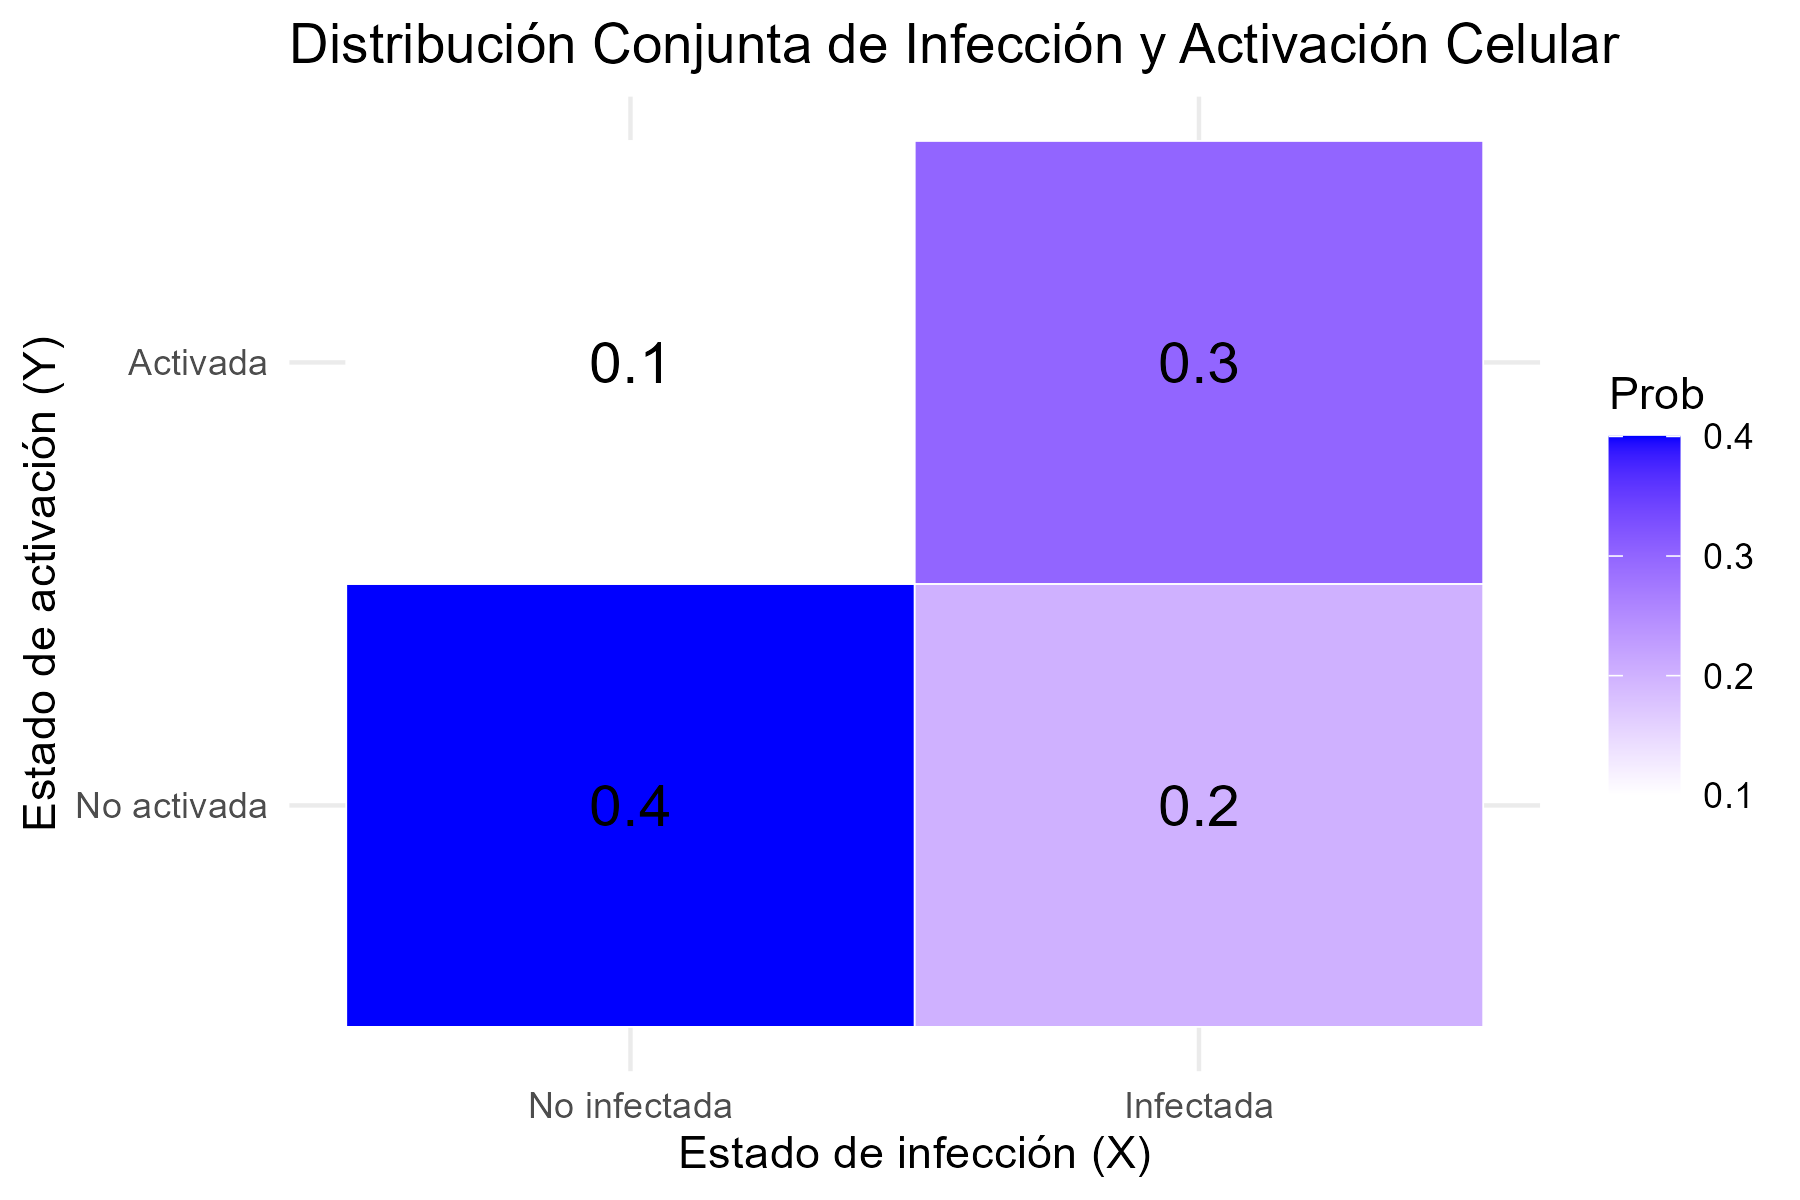
\includegraphics[width=0.8\linewidth]{images/distribucion_conjunta}

\subsection{Variable aleatorias bivariantes discretas}\label{variable-aleatorias-bivariantes-discretas}

Una vez introducidos los conceptos de forma general pasamos a estudiar el problema en el caso discreto, que es muy intuitivo y, a la vez permite introducir todos los conceptos relevantes.

Un \textbf{vector aleatorio discreto}, \((X, Y)\) es aquel cuyo recorrido o conjunto de valores posibles es finito o numerable.

En este caso, toda probabilidad

\[
P\{(X, Y) \in B\}, \quad \text{donde } B \text{ es un conjunto de posibles valores de } X, Y,
\]

se puede calcular a partir de la \textbf{función de masa de probabilidad discreta bivariante}.

\subsubsection{Función de masa de probabilidad discreta (fmp)}\label{funciuxf3n-de-masa-de-probabilidad-discreta-fmp}

La funcion de masa de probabilidad de los vectores aleatorios generaliza la función del mismo nombre en el caso univariante, es decir, es una función:

\[
f: \mathbb{R}^2 \to [0, 1]
\]

Que asigna la probabilidad a cada punto del plano: para todo \((x, y) \in \mathbb{R}^{2}\):

\[
f(x, y) = P\{w \in \Omega \mid X(w) = x, Y(w) = y\} = P[X = x, Y = y]
\]

\subsubsection{Propiedades de la fmp bivariante}\label{propiedades-de-la-fmp-bivariante}

\begin{itemize}
\tightlist
\item
  La masa total de probabilidad sobre el plano es 1:
\end{itemize}

\[
\sum_{(x_i, y_j) \in \mathbb{R}^{2}} f(x_i, y_j) = 1
\]

\begin{itemize}
\tightlist
\item
  Para todo subconjunto \(B \subseteq \mathbb{R}^2\), se verifica:
\end{itemize}

\[
F(x, y) = P[X \leq x, Y \leq y] = \sum_{x_i \leq x, y_j \leq y} f(x_i, y_j)
\]

Es decir, como en el caso univariante \emph{la función de distribución se puede calcular a partir de la función de masa de probabilidad}.

\paragraph{Intuición frente a construcción}\label{intuiciuxf3n-frente-a-construcciuxf3n}

La presentación de los conceptos anteriores suele generar cierto desasosiego entre los estudiantes que afrontan estos conceptos por primera (o siguientes) vez.

El motivo de este desasosiego es que el papel de la función de distribución no suele ser tan intuitivo como el de la función de masa de probabilidad.

Es decir, es más intuitivo pensar en como calcular lña probabilidad que la variable tome un valor concreto (\(P[X=x]\)) , que la probabilidad de que no alcance cierto valor (\(P[X\leq x]\)).

Sin embargo, la función que realmente permite transportar la probabilidad no es la función de masa de probabilidad (fmp) sino la función de distribución (fdd). De ahí el contraste entre intuición (fmp) y construcción (fdd)

\subsubsection{Ejemplo de distribución bivariante discreta}\label{ejemplo-de-distribuciuxf3n-bivariante-discreta}

Supongamos que un estudio mide el número de células infectadas y el número de linfocitos activados en un campo microscópico. Dado el tamaño del campo y el grado de infección los valores observados de cada variables son:

\begin{itemize}
\tightlist
\item
  \(X\): Número de células infectadas (\(X \in \{0, 1, 2, 3, 4, 5\}\))).
\item
  \(Y\): Número de linfocitos activados (\(Y \in \{0, 1, 2, 3\}\))).
\end{itemize}

La distribución conjunta se refleja en la siguiente tabla de probabilidades conjuntas:

\begin{longtable}[]{@{}ccccc@{}}
\toprule\noalign{}
\(P[X=x]\) & \(P[Y = 0]\) & \(P[Y = 1]\) & \(P[Y = 2]\) & \(P[Y = 3]\) \\
\midrule\noalign{}
\endhead
\bottomrule\noalign{}
\endlastfoot
0 & 0.12 & 0.06 & 0.02 & 0.00 \\
1 & 0.10 & 0.10 & 0.04 & 0.01 \\
2 & 0.06 & 0.12 & 0.08 & 0.02 \\
3 & 0.03 & 0.12 & 0.10 & 0.05 \\
4 & 0.01 & 0.08 & 0.12 & 0.06 \\
5 & 0.00 & 0.03 & 0.10 & 0.07 \\
\end{longtable}

Puede comprobarse como la suma de todos los valores de la tabla es 1, y calcular probabilidades de sucesos como

\textbf{Probabilidad de que hayan dos células infectadas y un linfocito:}

Para calcular la probabilidad de que haya exactamente 2 células infectadas y 1 linfocito activado, se puede usar el valor directamente de la tabla.

\[
P(X = 2, Y = 1) = 0.12
\]

\textbf{Probabilidad de que hayan menos de tres celulas infectadas y menos de dos linfocitos:}

Esta probabilidad es la suma de todas las combinaciones de \(X\) y \(Y\)) que cumplen con la condición de \(X < 3\)) y \(Y < 2\)). Es decir, sumamos las probabilidades de los casos

\((X = 0, Y = 0)\)), \((X = 0, Y = 1)\)), \((X = 1, Y = 0)\)), \((X = 1, Y = 1)\)), \((X = 2, Y = 0)\)), y \((X = 2, Y = 1)\)).

\[
P(X < 3, Y < 2) = P(X = 0, Y = 0) + P(X = 0, Y = 1) + P(X = 1, Y = 0) + P(X = 1, Y = 1) + P(X = 2, Y = 0) + P(X = 2, Y = 1)
\]

\[
P(X < 3, Y < 2) = 0.12 + 0.06 + 0.10 + 0.10 + 0.06 + 0.12 = 0.56
\]

Recordemos que, al tratarse de variables discretas, no es lo mismo \(P[X < x]\) que \(P[X \leq x]\), por lo que si la pregunta fuera ``Probabilidad de que hayan al menos tres celulas infectadas y al menos dos linfocitos'' deberíamos calcular:

\[
P(X \leq 3, Y \leq 2) 
\]
Esta última expresión se corresponde con la función de distribución evaluada en \((3,2)\).

\paragraph{Código R para el cálculo de la pmf}\label{cuxf3digo-r-para-el-cuxe1lculo-de-la-pmf}

Podemos hacer los cálculos usando R:

\begin{Shaded}
\begin{Highlighting}[]
\NormalTok{prob\_table }\OtherTok{\textless{}{-}} \FunctionTok{matrix}\NormalTok{(}\FunctionTok{c}\NormalTok{(}\FloatTok{0.12}\NormalTok{, }\FloatTok{0.06}\NormalTok{, }\FloatTok{0.02}\NormalTok{, }\FloatTok{0.00}\NormalTok{,}
                       \FloatTok{0.10}\NormalTok{, }\FloatTok{0.10}\NormalTok{, }\FloatTok{0.04}\NormalTok{, }\FloatTok{0.01}\NormalTok{,}
                       \FloatTok{0.06}\NormalTok{, }\FloatTok{0.12}\NormalTok{, }\FloatTok{0.08}\NormalTok{, }\FloatTok{0.02}\NormalTok{,}
                       \FloatTok{0.03}\NormalTok{, }\FloatTok{0.12}\NormalTok{, }\FloatTok{0.10}\NormalTok{, }\FloatTok{0.05}\NormalTok{,}
                       \FloatTok{0.01}\NormalTok{, }\FloatTok{0.08}\NormalTok{, }\FloatTok{0.12}\NormalTok{, }\FloatTok{0.06}\NormalTok{,}
                       \FloatTok{0.00}\NormalTok{, }\FloatTok{0.03}\NormalTok{, }\FloatTok{0.10}\NormalTok{, }\FloatTok{0.07}\NormalTok{), }
                     \AttributeTok{nrow =} \DecValTok{6}\NormalTok{, }\AttributeTok{byrow =} \ConstantTok{TRUE}\NormalTok{)}

\CommentTok{\# Asignar nombres a las filas y columnas}
\FunctionTok{rownames}\NormalTok{(prob\_table) }\OtherTok{\textless{}{-}} \DecValTok{0}\SpecialCharTok{:}\DecValTok{5}
\FunctionTok{colnames}\NormalTok{(prob\_table) }\OtherTok{\textless{}{-}} \DecValTok{0}\SpecialCharTok{:}\DecValTok{3}

\CommentTok{\# Mostrar la tabla}

\NormalTok{prob\_table}
\end{Highlighting}
\end{Shaded}

\begin{verbatim}
##      0    1    2    3
## 0 0.12 0.06 0.02 0.00
## 1 0.10 0.10 0.04 0.01
## 2 0.06 0.12 0.08 0.02
## 3 0.03 0.12 0.10 0.05
## 4 0.01 0.08 0.12 0.06
## 5 0.00 0.03 0.10 0.07
\end{verbatim}

\begin{Shaded}
\begin{Highlighting}[]
\CommentTok{\# Calcular la probabilidad de (X = 2, Y = 1)}
\NormalTok{prob\_X2\_Y1 }\OtherTok{\textless{}{-}}\NormalTok{ prob\_table[}\StringTok{"2"}\NormalTok{, }\StringTok{"1"}\NormalTok{]}
\FunctionTok{cat}\NormalTok{(}\StringTok{"P(X = 2, Y = 1) ="}\NormalTok{, prob\_X2\_Y1, }\StringTok{"}\SpecialCharTok{\textbackslash{}n}\StringTok{"}\NormalTok{)}
\end{Highlighting}
\end{Shaded}

\begin{verbatim}
## P(X = 2, Y = 1) = 0.12
\end{verbatim}

\begin{Shaded}
\begin{Highlighting}[]
\CommentTok{\# Calcular la probabilidad de (X \textless{} 3, Y \textless{} 2)}
\NormalTok{prob\_X\_lt\_3\_Y\_lt\_2 }\OtherTok{\textless{}{-}} \FunctionTok{sum}\NormalTok{(prob\_table[}\DecValTok{1}\SpecialCharTok{:}\DecValTok{3}\NormalTok{, }\DecValTok{1}\SpecialCharTok{:}\DecValTok{2}\NormalTok{])}
\FunctionTok{cat}\NormalTok{(}\StringTok{"P(X \textless{} 3, Y \textless{} 2) ="}\NormalTok{, prob\_X\_lt\_3\_Y\_lt\_2, }\StringTok{"}\SpecialCharTok{\textbackslash{}n}\StringTok{"}\NormalTok{)}
\end{Highlighting}
\end{Shaded}

\begin{verbatim}
## P(X < 3, Y < 2) = 0.56
\end{verbatim}

\paragraph{Código R para visualizar la distribución conjunta}\label{cuxf3digo-r-para-visualizar-la-distribuciuxf3n-conjunta}

Para visualizar la distribución conjunta, podemos usar el código siguiente;

\begin{Shaded}
\begin{Highlighting}[]
\CommentTok{\# Es preciso instalar y cargar el paquete scatterplot3d si no lo tienes instalado}
\CommentTok{\# install.packages("scatterplot3d")}
\FunctionTok{library}\NormalTok{(scatterplot3d)}

\CommentTok{\# Crear una matriz con los datos de la tabla de probabilidades}
\NormalTok{X\_vals }\OtherTok{\textless{}{-}} \FunctionTok{as.numeric}\NormalTok{(}\FunctionTok{rownames}\NormalTok{(prob\_table))}
\NormalTok{Y\_vals }\OtherTok{\textless{}{-}} \FunctionTok{as.numeric}\NormalTok{(}\FunctionTok{colnames}\NormalTok{(prob\_table))}

\CommentTok{\# Crear un grid de valores X e Y}
\NormalTok{X\_grid }\OtherTok{\textless{}{-}} \FunctionTok{rep}\NormalTok{(X\_vals, }\AttributeTok{each =} \FunctionTok{length}\NormalTok{(Y\_vals))}
\NormalTok{Y\_grid }\OtherTok{\textless{}{-}} \FunctionTok{rep}\NormalTok{(Y\_vals, }\AttributeTok{times =} \FunctionTok{length}\NormalTok{(X\_vals))}

\CommentTok{\# Extraer las probabilidades como un vector}
\NormalTok{Z\_vals }\OtherTok{\textless{}{-}} \FunctionTok{as.vector}\NormalTok{(prob\_table)}

\CommentTok{\# Enviar el gráfico 3D de barras simuladas a pdf}
\FunctionTok{png}\NormalTok{(}\StringTok{"images/pmfTrinomial.png"}\NormalTok{)}
\FunctionTok{scatterplot3d}\NormalTok{(X\_grid, Y\_grid, Z\_vals,}
                     \AttributeTok{type =} \StringTok{"h"}\NormalTok{, }\AttributeTok{color =} \StringTok{"lightblue"}\NormalTok{, }
                     \AttributeTok{pch =} \DecValTok{16}\NormalTok{, }\AttributeTok{lwd =} \DecValTok{5}\NormalTok{, }
                     \AttributeTok{cex.symbols =} \DecValTok{1}\NormalTok{,}
                     \AttributeTok{angle=}\DecValTok{60}\NormalTok{,}
                     \AttributeTok{xlab =} \StringTok{"Celulas Infectadas (X)"}\NormalTok{, }
                     \AttributeTok{ylab =} \StringTok{"Linfocitos Activados (Y)"}\NormalTok{, }
                     \AttributeTok{zlab =} \StringTok{"Probabilidad"}\NormalTok{,}
                     \AttributeTok{main =} \StringTok{"Distribución Conjunta de }\SpecialCharTok{\textbackslash{}n}\StringTok{ Celulas Infectadas y Linfocitos Activados"}\NormalTok{)}
\FunctionTok{dev.off}\NormalTok{()}
\end{Highlighting}
\end{Shaded}

\begin{verbatim}
## pdf 
##   2
\end{verbatim}

\begin{Shaded}
\begin{Highlighting}[]
\CommentTok{\# Añadir texto con los valores de las probabilidades en la parte superior de las barras}
\CommentTok{\# s3d$text(X\_grid, Y\_grid, Z\_vals, labels = round(Z\_vals, 2), pos = 3, col = "black")}
\end{Highlighting}
\end{Shaded}

\begin{Shaded}
\begin{Highlighting}[]
\NormalTok{knitr}\SpecialCharTok{::}\FunctionTok{include\_graphics}\NormalTok{(}\StringTok{"images/pmfTrinomial.png"}\NormalTok{, }\AttributeTok{rel\_path =} \ConstantTok{TRUE}\NormalTok{ )}
\end{Highlighting}
\end{Shaded}

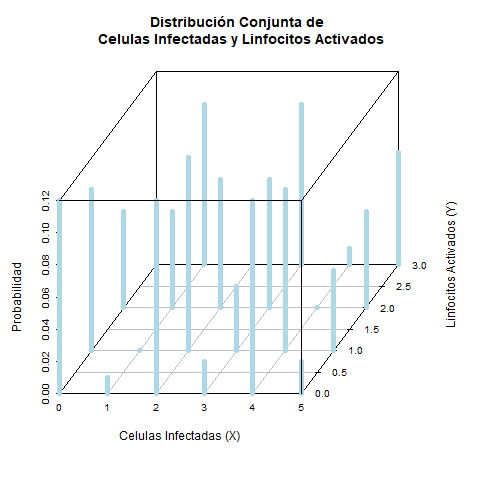
\includegraphics[width=0.9\linewidth]{images/pmfTrinomial}

\subsection{La distribución multinomial}\label{la-distribuciuxf3n-multinomial}

Antes de seguir con el estudio de las distribuciones discretas presentamos un caso importante de distribucion multivariante discreta, la \textbf{distribución multinomial}.

\subsubsection{Generación de las observaciones}\label{generaciuxf3n-de-las-observaciones}

Supongamos un experimentoaleatorio que puede producir \(k\) resultados posibles \(A_1, A_2, \dots, A_k\) con probabilidades \(p_1, p_2, \dots, p_k\), tales que \(p_1 + p_2 + \dots + p_k = 1\).

Repetimos el experimento \(n\) veces y llamamos \(X_1, X_2, \dots, X_k\) al número de veces que se presenta \(A_1, A_2, \dots, A_k\).

La distribución conjunta de \(X_1, X_2, \dots, X_k\) recibe el nombre de \textbf{multinomial}.

\subsubsection{Funcion de masa de probabilidad de la distribución multinomial}\label{funcion-de-masa-de-probabilidad-de-la-distribuciuxf3n-multinomial}

El vector \(\mathbf{X} = (X_1, \dots, X_k)\) tiene distribución multinomial de parámetros \(n\) y \(\mathbf{p} = (p_1, \dots, p_k),\) denotado por \(\mathbf{X} \sim \mathrm{M}(n, \mathbf{p})\), con \(n\) entero positivo, \(p_i \geq 0\) y \(\sum_{i=1}^{k} p_i = 1\).

Su función de densidad conjunta es:

\[
f(\mathbf{x}) = P[\mathbf{X} = \mathbf{x}] = \frac{n!}{x_1!x_2!\cdots x_k!} p_1^{x_1} p_2^{x_2} \dots p_k^{x_k}
\]

donde \(x_i\) son enteros no negativos tales que \(\sum_{i=1}^{k} x_i = n\).

\subsubsection{Relación con la distribución binomial}\label{relaciuxf3n-con-la-distribuciuxf3n-binomial}

Esta distribución puede verse como una generalización de la distribución binomial en el que, en lugar de tener dos posibles resultados, tenemos \(r\) resultados posibles.

\subsubsection{Un caso particular: La distribución trinomial}\label{un-caso-particular-la-distribuciuxf3n-trinomial}

Veamos un ejemplo propio del análisis de secuencias en el que se aplica esta distribución:

Si consideramos el alineamiento de dos secuencias \(x, y\) de tamaño \(n\), podemos observar:

\begin{itemize}
\tightlist
\item
  \$A\_1 \$: \(x_i\) alineado con \$y\_i \$, con \$P(A\_1) = p\_1 \$
\item
  \$A\_2 \$: \(x_i\) alineado con ``-'', con \$P(A\_2) = p\_2 \$
\item
  \$A\_3 \$: ``-'' alineado con \$y\_i \$, con \$P(A\_3) = 1 - p\_1 - p\_2 \$
\end{itemize}

La variable \$(X\_1, X\_2) \$, que cuenta el número de veces que se observa \(A_1, A_2\) (con \$X\_3 = n - X\_1 - X\_2 \$), sigue una distribución trinomial de parámetros \(n\), \$p\_1 \$, \$p\_2 \$.

Obsérvese que, dado que el total de observaciones \(n\) está prefijado, aunque haya tres categorías, \(A_1\), \(A_2\), \(A_3\) el número de observaciones de \(A_3\) es el total menos la suma de las observaciones de \(A_1+A_2\). O dicho de otra forma el número de probabilidades que són parámetros de la distribución es \(n-1=2\), lo que junto con \(n\) que es otyro parámetro determina que ``trinomial'' se refiera tanto al total de categorías como al número de parámetros, aunque, en realidad tan sólo hay dos componentes \(X_1\) y \(X_2\) independientes (concepto este que se definirá con precisión más adelante).

Estudiamos los posibles alineamientos de dos secuencias de 5 nucleótidos, en un contexto en el que las probabilidades de \(A_1\) y \(A_2\) son, respectivamente 0.6 y 0.2, es decir una Trinomial M(5; 0.6, 0.2) que dan lugar a la tabla siguiente.

\begin{longtable}[]{@{}ccccccc@{}}
\toprule\noalign{}
\(X_{1} \backslash X_{2}\) & 0 & 1 & 2 & 3 & 4 & 5 \\
\midrule\noalign{}
\endhead
\bottomrule\noalign{}
\endlastfoot
0 & (0,0,5) & (0,1,4) & (0,2,3) & (0,3,2) & (0,4,1) & (0,5,0) \\
1 & (1,0,4) & (1,1,3) & (1,2,2) & (1,3,1) & (1,4,0) & \\
2 & (2,0,3) & (2,1,2) & (2,2,1) & (2,3,0) & & \\
3 & (3,0,2) & (3,1,1) & (3,2,0) & & & \\
4 & (4,0,1) & (4,1,0) & & & & \\
5 & (5,0,0) & & & & & \\
\end{longtable}

A partir de la tabla anterior podemos determinar las probabilidades conjuntas:

\begin{longtable}[]{@{}ccccccc@{}}
\toprule\noalign{}
\(X_{1} \backslash X_{2}\) & 0 & 1 & 2 & 3 & 4 & 5 \\
\midrule\noalign{}
\endhead
\bottomrule\noalign{}
\endlastfoot
0 & 0.0003 & 0.0016 & 0.0032 & 0.0032 & 0.0016 & 0.0003 \\
1 & 0.0048 & 0.0192 & 0.0288 & 0.0192 & 0.0048 & \\
2 & 0.0288 & 0.0864 & 0.0864 & 0.0288 & & \\
3 & 0.0864 & 0.1728 & 0.0864 & & & \\
4 & 0.1296 & 0.1296 & & & & \\
5 & 0.0778 & & & & & \\
\end{longtable}

\subsection{Distribuciones marginales}\label{distribuciones-marginales}

\begin{itemize}
\item
  Dado un vector aleatorio, puede interesar el comportamiento individual de una o cada una de sus componentes \(X_i\).
\item
  La distribución de la componente \(i\)-ésima se denomina \textbf{distribución marginal} de \(X_i\).
\item
  Representa el comportamiento de \(X_i\) sin tener en cuenta las otras componentes, es decir, como si fuera una variable aleatoria unidimensional.
\end{itemize}

\subsubsection{Las marginales están en los márgenes}\label{las-marginales-estuxe1n-en-los-muxe1rgenes}

\begin{itemize}
\tightlist
\item
  El nombre de \textbf{distribución marginal} proviene del hecho de que en una distribución bivariada discreta como la trinomial, los valores de una fila coinciden con los valores de \(X_2\), y todos los de una columna con los de \(X_1\). Los valores en la fila 0 o columna 0 (los márgenes) representan precisamente las distribuciones marginales.
\end{itemize}

\subsubsection{Densidades marginales discretas}\label{densidades-marginales-discretas}

\begin{itemize}
\tightlist
\item
  La densidad marginal de \(X\) es:
\end{itemize}

\[
f_X(x) = f_1(x) = \sum_j f(x, y_j)
\]

y la de \(Y\) es:

\[
f_Y(y) = f_2(y) = \sum_i f(x_i, y)
\]

\subsubsection{Trinomial M(5; 0.6, 0.2): Distribuciones marginales}\label{trinomial-m5-0.6-0.2-distribuciones-marginales}

\begin{longtable}[]{@{}
  >{\centering\arraybackslash}p{(\columnwidth - 16\tabcolsep) * \real{0.1111}}
  >{\centering\arraybackslash}p{(\columnwidth - 16\tabcolsep) * \real{0.1111}}
  >{\centering\arraybackslash}p{(\columnwidth - 16\tabcolsep) * \real{0.1111}}
  >{\centering\arraybackslash}p{(\columnwidth - 16\tabcolsep) * \real{0.1111}}
  >{\centering\arraybackslash}p{(\columnwidth - 16\tabcolsep) * \real{0.1111}}
  >{\centering\arraybackslash}p{(\columnwidth - 16\tabcolsep) * \real{0.1111}}
  >{\centering\arraybackslash}p{(\columnwidth - 16\tabcolsep) * \real{0.1111}}
  >{\centering\arraybackslash}p{(\columnwidth - 16\tabcolsep) * \real{0.1111}}
  >{\centering\arraybackslash}p{(\columnwidth - 16\tabcolsep) * \real{0.1111}}@{}}
\toprule\noalign{}
\begin{minipage}[b]{\linewidth}\centering
\(X_1 \backslash X_2\)
\end{minipage} & \begin{minipage}[b]{\linewidth}\centering
0
\end{minipage} & \begin{minipage}[b]{\linewidth}\centering
1
\end{minipage} & \begin{minipage}[b]{\linewidth}\centering
2
\end{minipage} & \begin{minipage}[b]{\linewidth}\centering
3
\end{minipage} & \begin{minipage}[b]{\linewidth}\centering
4
\end{minipage} & \begin{minipage}[b]{\linewidth}\centering
5
\end{minipage} & \begin{minipage}[b]{\linewidth}\centering
\(X_2\)
\end{minipage} & \begin{minipage}[b]{\linewidth}\centering
\(P[X_2 = x]\)
\end{minipage} \\
\midrule\noalign{}
\endhead
\bottomrule\noalign{}
\endlastfoot
0 & (0,0,5) & (0,1,4) & (0,2,3) & (0,3,2) & (0,4,1) & (0,5,0) & 0 & 0.0102 \\
1 & (1,0,4) & (1,1,3) & (1,2,2) & (1,3,1) & (1,4,0) & & 1 & 0.0768 \\
2 & (2,0,3) & (2,1,2) & (2,2,1) & (2,3,0) & & & 2 & 0.2304 \\
3 & (3,0,2) & (3,1,1) & (3,2,0) & & & & 3 & 0.3456 \\
4 & (4,0,1) & (4,1,0) & & & & & 4 & 0.2592 \\
5 & (5,0,0) & & & & & & 5 & 0.0778 \\
X\_2 & 0 & 1 & 2 & 3 & 4 & 5 & & 1.0000 \\
\(P[X_2 = x]\) & 0.3277 & 0.4096 & 0.2048 & 0.0512 & 0.0064 & 0.0003 & 1.0000 & \\
\end{longtable}

\subsection{Distribuciones condicionales}\label{distribuciones-condicionales}

\begin{itemize}
\item
  A veces nos interesa la distribución de una componente si conocemos que la otra ha tomado un valor determinado.
\item
  En el ejemplo de los alineamientos, podríamos querer conocer los posibles valores y probabilidades de un alineamiento, si sabemos que hay exactamente un ``gap'' en la secuencia de prueba.
\end{itemize}

\subsubsection{Densidad condicional}\label{densidad-condicional}

¿Qué podemos decir de la distribución de \(Y\) si conocemos el valor de \(X\)?

\[
f(y \mid X = x) = P[Y = y \mid X = x] = \frac{P[X = x, Y = y]}{P[X = x]} = \frac{f(x, y)}{f_X(x)}
\]

siempre que \(f_X(x) > 0\).

\subsubsection{Trinomial M(5; 0.6, 0.2): Distribución condicional}\label{trinomial-m5-0.6-0.2-distribuciuxf3n-condicional}

Distribución de \(X_1\) condicionada a que \(X_2 = 1\).

\begin{longtable}[]{@{}lrrr@{}}
\toprule\noalign{}
\((X_1, 1)\) & \(P(X_1, 1)\) & \(P_{X_2}(1)\) & \(P(X_1 \mid X_2 = 1)\) \\
\midrule\noalign{}
\endhead
\bottomrule\noalign{}
\endlastfoot
(0,1,4) & 0.002 & 0.41 & 0.004 \\
(1,1,3) & 0.019 & 0.41 & 0.047 \\
(2,1,2) & 0.086 & 0.41 & 0.211 \\
(3,1,1) & 0.173 & 0.41 & 0.422 \\
(4,1,0) & 0.13 & 0.41 & 0.316 \\
Total & & & 1 \\
\end{longtable}

\subsection{Vectores aleatorios absolutamente continuos}\label{vectores-aleatorios-absolutamente-continuos}

\begin{itemize}
\tightlist
\item
  Diremos que \((X, Y)\) es absolutamente continua si existe una función \(f(x, y)\), llamada \textbf{función de densidad conjunta absolutamente continua} o \textbf{bivariada}, tal que, para todo \((x, y) \in \mathbb{R}^2\),
\end{itemize}

\[
F(x, y) = \int_{-\infty}^{x} \int_{-\infty}^{y} f(u, v)\, du \, dv
\]

\begin{itemize}
\tightlist
\item
  Si existe, la función de densidad absolutamente continua es única.
\end{itemize}

\subsubsection{Propiedades de la función de densidad conjunta}\label{propiedades-de-la-funciuxf3n-de-densidad-conjunta}

\begin{itemize}
\item
  \(f(x, y) \geq 0\)
\item
  La masa total de probabilidad es 1:
\end{itemize}

\[
\int_{-\infty}^{\infty} \int_{-\infty}^{\infty} f(x, y)\, dx\,dy = 1
\]

\begin{itemize}
\tightlist
\item
  Para cualquier conjunto \(S\):
\end{itemize}

\[
P\{(X, Y) \in S\} = \int_S f(x, y) \, dx \, dy
\]

En particular, la probabilidad de que \((X, Y)\) esté en un rectángulo:

\[
P(a_1 < X \leq a_2, b_1 < Y \leq b_2) = \int_{a_1}^{a_2} \int_{b_1}^{b_2} f(x, y) \, dx \, dy
\]

\subsubsection{Densidades marginales en el caso continuo}\label{densidades-marginales-en-el-caso-continuo}

\begin{itemize}
\tightlist
\item
  Las densidades marginales son:
\end{itemize}

\[
f_X(x) = \int_{-\infty}^{\infty} f(x, y) \, dy
\]

\[
f_Y(y) = \int_{-\infty}^{\infty} f(x, y) \, dx
\]

\subsubsection{Densidad condicional en el caso continuo}\label{densidad-condicional-en-el-caso-continuo}

\begin{itemize}
\tightlist
\item
  La densidad de \(Y\) condicionada a un valor de \(X\) es:
\end{itemize}

\[
f(y \mid X = x) = \frac{f(x, y)}{f_X(x)}
\]

siempre que \(f_X(x) > 0\).

\subsubsection{La Distribución Normal Bivariante}\label{la-distribuciuxf3n-normal-bivariante}

El ejemplo más importante de una distribución de probabilidad absolutamente continua para vectores aleatorios es la \textbf{distribución normal bivariante}. Esta distribución describe dos variables aleatorias continuas, \(X\) y \(Y\), cuya relación está modelada por una correlación lineal y tiene forma de campana (gaussiana) en dos dimensiones.

\paragraph{Función de Densidad Conjunta}\label{funciuxf3n-de-densidad-conjunta}

La función de densidad conjunta de la distribución normal bivariante con medias \(\mu_X\), \(\mu_Y\), desviaciones estándar \(\sigma_X\), \(\sigma_Y\) y coeficiente de correlación \(\rho\) es:

\[
f(x, y) = \frac{1}{2 \pi \sigma_X \sigma_Y \sqrt{1 - \rho^2}} \exp \left( -\frac{1}{2(1 - \rho^2)} \left[ \frac{(x - \mu_X)^2}{\sigma_X^2} + \frac{(y - \mu_Y)^2}{\sigma_Y^2} - \frac{2\rho(x - \mu_X)(y - \mu_Y)}{\sigma_X \sigma_Y} \right] \right)
\]

Esta expresión se generaliza fácilmente de la distribución normal univariante, pero en este caso incluye términos adicionales que representan la interacción entre \(X\) y \(Y\).

\paragraph{Ejemplo}\label{ejemplo}

En vez de proporcionar un código para visualizar la distribución normal bivariante podéis seguir este enlace: \url{https://datasciencegenie.com/3d-contour-plots-of-bivariate-normal-distribution/} en donde se extiende lo que acabamos de discutir y se proporciona algunos ejemplos con R.

\paragraph{Distribuciones Marginales}\label{distribuciones-marginales-1}

Para obtener las \textbf{distribuciones marginales} a partir de una \textbf{normal bivariante}, debemos integrar la densidad conjunta sobre una de las variables. Dado que estamos trabajando con una distribución normal bivariante, su densidad conjunta está dada por:

\[
f_{X,Y}(x, y) = \frac{1}{2 \pi \sigma_X \sigma_Y \sqrt{1 - \rho^2}} \exp\left( -\frac{1}{2(1 - \rho^2)} \left[ \frac{(x - \mu_X)^2}{\sigma_X^2} + \frac{(y - \mu_Y)^2}{\sigma_Y^2} - \frac{2\rho(x - \mu_X)(y - \mu_Y)}{\sigma_X \sigma_Y} \right] \right)
\]

Para obtener la \textbf{marginal de \(X\)}, debemos integrar sobre \(Y\):

\[
f_X(x) = \int_{-\infty}^{\infty} f_{X,Y}(x, y) \, dy
\]

Al realizar esta integral, se obtiene que la distribución marginal de \(X\) es:

\[
f_X(x) = \frac{1}{\sqrt{2 \pi \sigma_X^2}} \exp\left( -\frac{(x - \mu_X)^2}{2 \sigma_X^2} \right)
\]

Esto muestra que \(X\) sigue una distribución normal con media \(\mu_X\) y varianza \(\sigma_X^2\), es decir, \(X \sim N(\mu_X, \sigma_X^2)\).

Del mismo modo, para la \textbf{marginal de \(Y\)}, integramos sobre \(X\):

\[
f_Y(y) = \int_{-\infty}^{\infty} f_{X,Y}(x, y) \, dx
\]

La solución de esta integral da:

\[
f_Y(y) = \frac{1}{\sqrt{2 \pi \sigma_Y^2}} \exp\left( -\frac{(y - \mu_Y)^2}{2 \sigma_Y^2} \right)
\]

Lo que significa que \(Y\) sigue una distribución normal con media \(\mu_Y\) y varianza \(\sigma_Y^2\), es decir, \(Y \sim N(\mu_Y, \sigma_Y^2)\).

\paragraph{Ejemplo}\label{ejemplo-1}

Supongamos que tenemos una distribución normal bivariante con los siguientes parámetros:

\begin{itemize}
\tightlist
\item
  \(\mu_X = 100\), \(\sigma_X = 15\)
\item
  \(\mu_Y = 50\), \(\sigma_Y = 10\)
\item
  \(\rho = 0.5\)
\end{itemize}

La densidad conjunta es:

\[
f_{X,Y}(x, y) = \frac{1}{2 \pi (15)(10) \sqrt{1 - 0.5^2}} \exp\left( -\frac{1}{2(1 - 0.5^2)} \left[ \frac{(x - 100)^2}{15^2} + 
       \frac{(y - 50)^2}{10^2} - \frac{2(0.5)(x - 100)(y - 50)}{(15)(10)} \right] \right)
\]

Integrando sobre \(Y\), obtenemos la distribución marginal de \(X\):

\[
f_X(x) = \frac{1}{\sqrt{2 \pi (15^2)}} \exp\left( -\frac{(x - 100)^2}{2 \cdot 15^2} \right)
\]

De manera análoga, la marginal de \(Y\) es:

\[
f_Y(y) = \frac{1}{\sqrt{2 \pi (10^2)}} \exp\left( -\frac{(y - 50)^2}{2 \cdot 10^2} \right)
\]

\subsubsection{Distribuciones Condicionales}\label{distribuciones-condicionales-1}

La distribución condicional de una variable dado un valor específico de la otra también es normal univariante. Por ejemplo, la distribución condicional de \(X\) dado \(Y = y\) es:

\[
X \mid Y = y \sim N \left( \mu_X + \rho \frac{\sigma_X}{\sigma_Y} (y - \mu_Y), (1 - \rho^2)\sigma_X^2 \right)
\]

De forma análoga, la distribución condicional de \(Y\) dado \(X = x\) es:

\[
Y \mid X = x \sim N \left( \mu_Y + \rho \frac{\sigma_Y}{\sigma_X} (x - \mu_X), (1 - \rho^2)\sigma_Y^2 \right)
\]

\paragraph{Ejemplo}\label{ejemplo-2}

Podemos calcular la distribución condicional de \(X\) dado que \(Y = 180\) cm, y mostrar cómo cambia la distribución de \(X\) bajo esta condición:

\begin{Shaded}
\begin{Highlighting}[]
\CommentTok{\# Valores originales}
\NormalTok{mu }\OtherTok{\textless{}{-}} \FunctionTok{c}\NormalTok{(}\DecValTok{100}\NormalTok{, }\DecValTok{50}\NormalTok{)}
\NormalTok{sigma }\OtherTok{\textless{}{-}} \FunctionTok{c}\NormalTok{(}\DecValTok{15}\NormalTok{, }\DecValTok{10}\NormalTok{)}
\NormalTok{rho }\OtherTok{\textless{}{-}} \FloatTok{0.5}

\CommentTok{\# Condicionar X dado Y = 180}
\NormalTok{y\_cond }\OtherTok{\textless{}{-}} \DecValTok{180}
\NormalTok{mu\_cond }\OtherTok{\textless{}{-}}\NormalTok{ mu[}\DecValTok{1}\NormalTok{] }\SpecialCharTok{+} \FloatTok{0.6} \SpecialCharTok{*}\NormalTok{ (}\DecValTok{10}\SpecialCharTok{/}\DecValTok{7}\NormalTok{) }\SpecialCharTok{*}\NormalTok{ (y\_cond }\SpecialCharTok{{-}}\NormalTok{ mu[}\DecValTok{2}\NormalTok{])}
\NormalTok{sigma\_cond }\OtherTok{\textless{}{-}} \FunctionTok{sqrt}\NormalTok{(}\DecValTok{1} \SpecialCharTok{{-}} \FloatTok{0.6}\SpecialCharTok{\^{}}\DecValTok{2}\NormalTok{) }\SpecialCharTok{*} \DecValTok{10}

\CommentTok{\# Mostrar la media y desviación estándar condicionales}
\NormalTok{mu\_cond}
\end{Highlighting}
\end{Shaded}

\begin{verbatim}
## [1] 211.4286
\end{verbatim}

\begin{Shaded}
\begin{Highlighting}[]
\NormalTok{sigma\_cond}
\end{Highlighting}
\end{Shaded}

\begin{verbatim}
## [1] 8
\end{verbatim}

Esto nos dice que el peso medio de una persona con altura de 180 cm es mayor que el peso medio de la población total, y su desviación estándar es menor debido a la correlación positiva entre peso y altura.

\subsection{Independencia de variables aleatorias}\label{independencia-de-variables-aleatorias}

Una vez introducido el concepto de distribución conjunta pasamos a estudiar un caso particularmente importante de distribución conjunta, la independencia.
De forma aparentemente contradictoria, en este caso, las variables se caracterizan por el hecho de que \emph{no varían conjuntamente} sino que lo hacen \emph{independientemente} las unas de las otras.

De manera intuitiva podemos decir que dos variables aleatorias son independientes si los valores que toma una de ellas no afectan a los de la otra ni a sus probabilidades.

En muchas ocasiones la independencia será evidente a partir del experimento, por ejemplo, es independiente el resultado del lanzamiento de un dado y el de una moneda tres veces. Por tanto las variables:

\begin{itemize}
\tightlist
\item
  \(X_1\): ``Puntuación obtenida con el dado'' y
\item
  \(X_2\): ``Número de caras obtenidas al lanzar tres veces una moneda'' serán variables independientes.
\end{itemize}

En otras ocasiones tenemos una dependencia clara, por ejemplo, al lanzar un dado consideremos las variables

\begin{itemize}
\tightlist
\item
  \(Y_1=\): puntuación del dado,
\item
  \(Y_2=\): variable indicadora de puntuación par.
\end{itemize}

Es evidente que existe una clara dependencia, si sabemos que \(Y=1\), la variable \(X\) sólo puede tomar los valores 2 , 4 o 6 ; si sabemos que \(X=3\), entonces, \(Y=0\) forzosamente.

Algunas veces podemos suponer la existencia de una cierta relación entre variables, aunque sea en forma algo abstracta y sin concretar. Por ejemplo si realizamos unas mediciones sobre unos individuos, las variables altura en cm y peso en Kg probablemente estarán relacionadas, los valores de una influirán en los valores de la otra. Intentar determinar la naturaleza exacta de la relación entre ambas es lo que en estadística conocemos como un problema de correlación (si nos interesa unicamente la asociación) o de regresión (si uqeremos modelizar una variable en función d ela otra).

Si queremos una definición algo más formal, basta con que recordemos que dos sucesos son independientes si la probabilidad de la intersección es igual al producto de probabilidades, aplicando esta definición a sucesos del tipo \(X \leq a\) tenemos la definición siguiente:

\subsubsection{Primera caracterización de la independencia}\label{primera-caracterizaciuxf3n-de-la-independencia}

Diremos que dos variables aleatorias \(X\) e \(Y\) son independientes si y sólo si su función de distribución conjunta puede expresarse como el producto de las funciones de distribución marginales, es decir si

\[
F_{X,Y}(x,y)= P\left( (X \leq x) \cap (Y \leq b)\right)=P(X \leq x) \times P(Y \leq y)=F_{X}(x) \times F_{Y}(y)
\]

Fijémonos que, como en otros casos, la función que nos permite caracterizar una condición de forma general es la función de distribución.

\paragraph{Variables discretas independientes}\label{variables-discretas-independientes}

En el caso de las variables discretas la caracterización de la independencia puede hacerse, además, por las funciones de masa de probabilidad:

Diremos que dos variables aleatorias \textbf{discretas} \(X\) e \(Y\) son independientes si y sólo si su función de masa de probabilidad conjunta puede expresarse como el producto de las funciones de masa de probabilidad marginales, es decir si

\[
f_{X,Y}(x,y)= P\left( (X = x) \cap (Y = y)\right)=P(X = x) \times P(Y = y)=f_{X}(x) \times f_{Y}(y)
\]

\subsubsection{Propiedades de las variables independientes}\label{propiedades-de-las-variables-independientes}

Como consecuencia inmediata de la independencia de \(X\) e \(Y\), se cumple lo siguiente:

\[
P(a<X \leq c \cap b<Y \leq d)=P(a<X \leq c) \cdot P(b<Y \leq d)
\]
Que podría re-enunciarse diciendo que la probabilidad conjunta en un rectangulo definido por los valores ``a, c, b, d'' es el producto de las probabilidades marginales en los segmentos ``ac'', para \(X\) y ``bd'' para \(Y\).

\subsection{Momentos de vectores aleatorios}\label{momentos-de-vectores-aleatorios}

Una vez hemos introducido los vectores aleatorios, que como hemos señalado, son variables aleatorias bi, tri o \(n\)-dimensionales tiene sentido preguntarse como se extienden a dichos vectores los conceptos y propiedades que introdujimos para variables aleatorias unidimensionales.

Ya hemos visto como, para las funciones de probabilidad, la función de densidad o la función de distribución, existen extensiones imediatas, la función de densidad conjunta o la función de distribución conjunmta.

Hemos visto también que, además de dichas extensiones, aparecen nuevos conceptos, que sólo tienen sentido en dos o más dimensiones, como las funciones de densidad condicionales o funciones de densidad marginales.

Al considerar conceptos como la media o la varianza veremos que sucede algo similar:

\begin{itemize}
\tightlist
\item
  Por un lado conceptos como el de esperanza se extiende imediatamente al vector de medias.
\item
  Por otro, conceptos como la varianza, han de tener en cuenta ahora, la posibilidad de variación conjunta entre dos o más variables lo que lleva a introducir magnitudes como la covarianza y la correlación.

  \begin{itemize}
  \tightlist
  \item
    La extensión del concepto de varianza pasa ahora a combinar extensiones y conceptos nuevos en lo que se conoce como matriz de varianzas-covarianzas.
  \end{itemize}
\end{itemize}

\subsubsection{Esperanza de un vector aleatorio o vector de medias}\label{esperanza-de-un-vector-aleatorio-o-vector-de-medias}

La \textbf{esperanza matemática} de un vector aleatorio es un vector que contiene las esperanzas matemáticas de cada una de las componentes de dicho vector.

Si tenemos un vector aleatorio bivariante \(\mathbf{X}=(X_1,X_2)\), su esperanza \(\mathbb{E}(\mathbf{X})\) está dada por:

\[
\mathbb{E}(\mathbf{X})=
\begin{pmatrix}
\mathbb{E}(X_1)\\
\mathbb{E}(X_2)
\end{pmatrix}
\]

Consideremos un experimento en el que estamos midiendo el nivel de expresión génica de dos genes \(X_1\) y \(X_2\) en una muestra de células. Si los niveles promedio de expresión son \(\mu_1=5\) y \(\mu_2=8\), entonces la esperanza del vector aleatorio sería:

\[
\mathbb{E}(\mathbf{X})=
\begin{pmatrix}
5\\
8
\end{pmatrix}
\]

\subsubsection{Covarianza entre dos variables aleatorias}\label{covarianza-entre-dos-variables-aleatorias}

La \textbf{covarianza} entre dos variables aleatorias \(X_1\) y \(X_2\) es una medida del grado de dependencia \emph{lineal} entre ellas.

La covarianza se define como

\[
\text{Cov}(X_1,X_2)=\mathbb{E}[(X_1-\mathbb{E}(X_1))(X_2-\mathbb{E}(X_2))]
\]

Supongamos que estamos midiendo la cantidad de dos metabolitos \(X_1\) y \(X_2\) en una muestra, y queremos saber si sus concentraciones tienden a aumentar o disminuir juntas. Si obtenemos una covarianza de 0.5, y conocemos la escala en que varían los datos, podemos concluir que existe ligera tendencia a que los aumentos en \(X_1\) estén asociados con aumentos en \(X_2\).

\subsubsection{Covarianza y correlación}\label{covarianza-y-correlaciuxf3n}

El ejemplo anterior es claramente insatisfactorio, puesto que valores de 0.5 pueden sugerir una gran dependencia o cas ninguna, segun cual sea la escala o el rango de variación de los valores que se consideran.

Para evitar esta arbitrariedad se introduce la correlación lineal.

La \textbf{correlación} entre dos variables aleatorias es una medida estandarizada del grado de dependencia lineal entre dos variables (es decir de lacovarianza), que toma valores entre -1 y 1 y que se define como:

\[
\text{Corr}(X_1,X_2)=\frac{\text{Cov}(X_1,X_2)}{\sqrt{\text{Var}(X_1)\text{Var}(X_2)}}
\]

En el caso de los metabolitos mencionados anteriormente, si \(\text{Cov}(X_1,X_2)=0.5\), \(\text{Var}(X_1)=2\) y \(\text{Var}(X_2)=3\), podemos calcular la correlación, que valdría:

\[
\text{Corr}(X_1,X_2)=\frac{0.5}{\sqrt{2\times 3}}=\frac{0.5}{\sqrt{6}}\approx 0.204
\]

Esto indica una correlación positiva débil entre las concentraciones de los dos metabolitos.

Obsérvese, sin embargo que si en vez de los valores anteriores para las varianzas de \(X\) e \(Y\) hubiéramos tenido \(\text{Var}(X_1)=1\) y \(\text{Var}(X_2)=.5\) el valor de la correlación habría sido:

\[
\text{Corr}(X_1,X_2)=\frac{0.5}{\sqrt{1\times 0.5}}=\frac{0.5}{\sqrt{0.5}}\approx 0.7071
\]
Este ejemplo muestra como la correlación aporta más información sobre la dependencia lineal, puesto que, además de tener en cuenta la variación conjunta, tiene en cuenta la variabilidad individual de cada componente.

\subsubsection{Matriz de varianzas-covarianzas}\label{matriz-de-varianzas-covarianzas}

La \textbf{matriz de varianzas-covarianzas} de un vector aleatorio \(\mathbf{X}=(X_1,X_2)\) es una matriz que contiene las varianzas de las componentes en la diagonal y las covarianzas fuera de la diagonal. Está definida como:

\[
\text{Cov}(\mathbf{X})=
\begin{pmatrix}
\text{Var}(X_1)&\text{Cov}(X_1,X_2)\\
\text{Cov}(X_2,X_1)&\text{Var}(X_2)
\end{pmatrix}
\]

Siguiendo con el ejemplo de los metabolitos, si \(\text{Var}(X_1)=2\), \(\text{Var}(X_2)=3\), y la covarianza es \(0.5\), la matriz de covarianzas sería:

\[
\text{Cov}(\mathbf{X})=
\begin{pmatrix}
2&0.5\\
0.5&3
\end{pmatrix}
\]

Esto nos indica la dispersión de cada variable y la relación entre ambas.

\textbf{La distribución normal bivariante}

Una de las distribuciones más importantes que describe el comportamiento conjunto de dos variables aleatorias es la \textbf{distribución normal bivariante}.

Un vector aleatorio \(\mathbf{X}=(X_1,X_2)\) tiene una distribución normal bivariante si su función de densidad conjunta está dada por:

\[
f(x_1,x_2)=\frac{1}{2\pi\sigma_1\sigma_2\sqrt{1-\rho^2}}\exp\left(-\frac{1}{2(1-\rho^2)}\left[\frac{(x_1-\mu_1)^2}{\sigma_1^2}-2\rho\frac{(x_1-\mu_1)(x_2-\mu_2)}{\sigma_1\sigma_2}+\frac{(x_2-\mu_2)^2}{\sigma_2^2}\right]\right)
\]

Aquí, \(\mu_1\) y \(\mu_2\) son las medias de \(X_1\) y \(X_2\), \(\sigma_1^2\) y \(\sigma_2^2\) son las varianzas, y \(\rho\) es el coeficiente de correlación.

\subsubsection{Matriz de correlaciones}\label{matriz-de-correlaciones}

La \textbf{matriz de correlaciones} de un vector aleatorio bivariante \(\mathbf{X}=(X_1,X_2)\) es una matriz simétrica \(2\times 2\) que contiene los coeficientes de correlación entre las componentes \(X_1\) y \(X_2\). La correlación mide la relación lineal entre las variables y se define como:

\[
\text{Corr}(X_1,X_2)=\frac{\text{Cov}(X_1,X_2)}{\sqrt{\text{Var}(X_1)\text{Var}(X_2)}}
\]

La matriz de correlaciones \(\text{Corr}(\mathbf{X})\) está dada por:

\[
\text{Corr}(\mathbf{X})=
\begin{pmatrix}
1 & \text{Corr}(X_1,X_2)\\
\text{Corr}(X_2,X_1) & 1
\end{pmatrix}
\]

Dado que \(\text{Corr}(X_1,X_2)=\text{Corr}(X_2,X_1)\), la matriz es simétrica, y los elementos diagonales son siempre \(1\) porque la correlación de una variable consigo misma es \(1\).

\paragraph{Relación con la matriz de covarianzas}\label{relaciuxf3n-con-la-matriz-de-covarianzas}

La matriz de correlaciones está relacionada con la \textbf{matriz de covarianzas} de la forma siguiente:

Si \(\Sigma\) es la matriz de covarianzas de \(\mathbf{X}=(X_1,X_2)\), con \(\Sigma=\begin{pmatrix} \text{Var}(X_1) & \text{Cov}(X_1,X_2)\\ \text{Cov}(X_2,X_1) & \text{Var}(X_2) \end{pmatrix}\), la matriz de correlaciones se obtiene ``normalizando'' cada covarianza dividiendo por el producto de las desviaciones estándar de las respectivas variables:

\[
\text{Corr}(\mathbf{X})=
\begin{pmatrix}
1 & \frac{\text{Cov}(X_1,X_2)}{\sigma_1\sigma_2}\\
\frac{\text{Cov}(X_2,X_1)}{\sigma_1\sigma_2} & 1
\end{pmatrix}
\]

donde \(\sigma_1=\sqrt{\text{Var}(X_1)}\) y \(\sigma_2=\sqrt{\text{Var}(X_2)}\).

Supongamos que medimos dos variables, como la altura \(X_1\) y el peso \(X_2\) de un grupo de personas. Sabemos que:

\begin{itemize}
\tightlist
\item
  \(\text{Var}(X_1)=25\) (varianza de la altura),
\item
  \(\text{Var}(X_2)=100\) (varianza del peso),
\item
  \(\text{Cov}(X_1,X_2)=40\) (covarianza entre altura y peso).
\end{itemize}

La \textbf{matriz de covarianzas} sería:

\[
\Sigma=
\begin{pmatrix}
25 & 40\\
40 & 100
\end{pmatrix}
\]

La correlación entre \(X_1\) y \(X_2\) se calcula como:

\[
\text{Corr}(X_1,X_2)=\frac{40}{\sqrt{25 \times 100}}=\frac{40}{50}=0.8
\]

Por lo tanto, la \textbf{matriz de correlaciones} será:

\[
\text{Corr}(\mathbf{X})=
\begin{pmatrix}
1 & 0.8\\
0.8 & 1
\end{pmatrix}
\]

Esto indica una fuerte correlación positiva entre la altura y el peso de las personas en este grupo. La matriz de correlaciones nos proporciona una forma normalizada de comparar la dependencia entre las variables, sin depender de las unidades de medida.

\subsubsection{Segunda caracterización de la independencia}\label{segunda-caracterizaciuxf3n-de-la-independencia}

La \textbf{independencia} entre dos variables aleatorias \(X_1\) y \(X_2\) puede caracterizarse también a través de sus \textbf{esperanzas} de la siguiente manera:

Dos variables son \textbf{independientes} si la esperanza del producto de ambas es igual al producto de las esperanzas de cada una por separado. Es decir si se verifica que:

\[
\mathbb{E}[X_1 X_2] = \mathbb{E}[X_1] \mathbb{E}[X_2]
\]

Esta propiedad refleja que, cuando las variables son independientes, el valor esperado del producto no se ve afectado por la interacción entre ellas, lo que implica que no hay dependencia entre las dos.

Una consecuencia importante de esta propiedad es cómo afecta a la \textbf{covarianza} entre \(X_1\) y \(X_2\).

Si \(X_1\) y \(X_2\) son \textbf{independientes}, entonces, por la propiedad anterior, \(\mathbb{E}[X_1 X_2] = \mathbb{E}[X_1] \mathbb{E}[X_2]\) lo que, a su vez, significa que la covarianza es cero:

\[
\text{Cov}(X_1, X_2) = \mathbb{E}[X_1]\mathbb{E}[X_2] - \mathbb{E}[X_1]\mathbb{E}[X_2] = 0
\]

Por lo tanto, \textbf{si dos variables son independientes, necesariamente su covarianza es cero}.

Sin embargo, la inversa no es cierta: el hecho de que la covarianza sea cero no implica que las variables sean independientes.

\subsubsection{Relación entre incorrelación e independencia}\label{relaciuxf3n-entre-incorrelaciuxf3n-e-independencia}

Cuando la covarianza entre dos variables es cero, se dice que las variables son \textbf{incorreladas}.
Aunque la \textbf{independencia} implica que las variables son incorreladas, lo contrario no siempre es verdad: dos variables pueden ser incorreladas (tener covarianza cero) pero \textbf{no independientes}.

Un ejemplo clásico es el siguiente: si consideramos una variable aleatoria \(X\) y definimos \(Y = X^2\), entonces, aunque la covarianza entre \(X\) y \(Y\) puede ser cero (especialmente si \(X\) tiene una distribución simétrica alrededor de 0, como la normal estándar), \(X\) y \(Y\) no son independientes, porque el valor de \(Y\) está completamente determinado por \(X\).

Consideremos dos variables aleatorias \(X_1\) y \(X_2\) que siguen una distribución normal conjunta bivariante con media cero:

\[
(X_1, X_2) \sim \mathcal{N}\left(\mathbf{0}, \Sigma \right)
\]

Si la \textbf{matriz de covarianzas} \(\Sigma\) es diagonal, es decir, \(\text{Cov}(X_1, X_2) = 0\), entonces \(X_1\) y \(X_2\) son incorreladas.

En este caso particular, cuando las variables son normales, la incorrelación \textbf{sí} implica independencia, porque en distribuciones normales la ausencia de correlación (covarianza cero) también implica que no hay ninguna dependencia entre las variables.

Sin embargo, en otras distribuciones que no son normales, la incorrelación no garantiza la independencia, lo que subraya la importancia de distinguir entre los dos conceptos.

\section{Grandes muestras}\label{grandes-muestras}

Este capítulo está pendiente de revisión, para corregir posibles problemas derivados de la importación, desde la antigua version en HTML, a la versión actual.

Estos problemas siempre serán \emph{estéticos y no conceptuales}, por lo que la lectura del texto en su estado actual no inducirá a errores conceptuales en ningún caso.

La primera sección, además, está pendiente de ser introducida en los apuntes.

La versión actualizada estará disponible en el momento de inicio de la actividad, durante el semestre actual (2024-25-S1).

\subsection{Introducción: Aproximaciones asintóticas}\label{introducciuxf3n-aproximaciones-asintuxf3ticas}

\subsubsection{Convergencia de variables aleatorias}\label{convergencia-de-variables-aleatorias}

\subsection{Leyes de los grandes números}\label{leyes-de-los-grandes-nuxfameros}

\subsection{El teorema central del límite}\label{el-teorema-central-del-luxedmite}

El teorema central del límite (a partir de ahora, TCL) presenta un doble interés. Por un lado, proporciona a la estadística un resultado crucial para abordar el estudio de la distribución asintótica de muchos tipos de variables aleatorias. Como se verá en próximos capítulos, va a resultar básico en la construcción de contrastes de hipótesis y de intervalos de confianza, dos herramientas esenciales en estadística aplicada.

Además, el TCL proporciona una explicación teórica fundamentada a un fenómeno habitual en experimentos reales: las variables estudiadas presentan muchas veces una distribución empírica aproximadamente normal.

El TCL forma parte de un conjunto de propiedades relativas a las convergencias de variables aleatorias. En este tema se estudia sólo un tipo de convergencia, la convergencia en ley, ya que es necesaria para entender el enunciado del TCL. Se descarta, pues, en este documento el estudio de los otros tipos de convergencias (en probabilidad, casi segura, etc.) y el estudio de las leyes de los grandes números.

Posiblemente el lector con poca formación en análisis matemático hallará alguna dificultad en la primera lectura de la definición de convergencia en ley y en el enunciado del TCL. Si es este el caso, los ejemplos incluidos han de ayudar en su comprensión. Consideramos al TCL un resultado básico con el que hay que familiarizarse, ya que se aplicará repetidamente en los próximos temas.

\subsubsection{Sumas de variables aleatorias}\label{sumas-de-variables-aleatorias}

El TCL estudia el comportamiento de las sumas de variables aleatorias. En temas anteriores se han visto ya ejemplos de sumas de variables aleatorias.

Formalmente, la suma de dos variables aleatorias corresponde a la siguiente aplicación: si \(X_{1}\) y \(X_{2}\) son dos variables aleatorias definidas sobre \(\Omega\), la suma es:

\[
\begin{aligned}
X_{1}+X_{2}: & \Omega \rightarrow \mathbb{R} \\
& \omega \mapsto X_{1}(\omega)+X_{2}(\omega)
\end{aligned}
\]

La suma de dos variables puede extenderse sin dificultad a sumas de tres, cuatro,\ldots{} y, en general, \(n\) variables aleatorias.

El TCL se ocupa de las sucesiones de variables aleatorias. En el contexto del TCL una sucesión corresponde a un conjunto donde el primer elemento es una variable aleatoria, el segundo elemento es la suma de dos variables aleatorias, el tercero es la suma de tres variables aleatorias, y así sucesivamente.

Una sucesión es un conjunto de elementos infinitos, que se designan simbólicamente mediante \(\left\{X_{n}\right\}\).
Cada uno de los elementos de la sucesión (que es una variable aleatoria) lleva asociada una determinada función de distribución:

\[
X_{n} \rightarrow F_{n}
\]

Así pues, la sucesión de variables aleatorias lleva asociada una secuencia paralela de funciones de distribución.

En los ejemplos se presentan sumas de variables aleatorias de diferentes tipos.

\paragraph{Presentación de los ejemplos}\label{presentaciuxf3n-de-los-ejemplos}

\begin{enumerate}
\def\labelenumi{\arabic{enumi}.}
\tightlist
\item
  Ejemplo 1: sumas de variables binomiales.
\item
  Ejemplo 2: sumas de variables Poisson.
\item
  Ejemplo 3: sumas de \(n\) puntuaciones de dados.
\item
  Ejemplo 4: sumas de variables uniformes.
\item
  Ejemplo 5: sumas de variables exponenciales.
\end{enumerate}

\subsubsection{Definición de convergencia en ley}\label{definiciuxf3n-de-convergencia-en-ley}

La siguiente definición se ocupa del comportamiento de las sucesiones.
Sea \(\left\{X_{n}\right\}\) una sucesión de variables aleatorias, y sea \(\left\{F_{n}\right\}\) la correspondiente sucesión de funciones de distribución. Se dice que \(\left\{X_{n}\right\}\) converge en ley a una variable aleatoria \(X\) de función de distribución \(F\) si:

\[
\lim _{n \rightarrow \infty} F_{n}(x)=F(x) \quad \text { para todo } \mathrm{x} \text { donde } F \text { es contínua. }
\]

Se indica que la sucesión converge en ley mediante el símbolo:

\[
X_{n} \stackrel{\mathrm{L}}{\rightarrow} X
\]

El significado de la definición es que, al aumentar arbitrariamente \(n\), las sucesivas funciones de distribución de la secuencia se aproximan a la distribución \(F\) de la variable \(X\).

En los ejemplos se presentan gráficamente algunas situaciones donde diferentes sucesiones de variables aleatorias convergen en ley a una variable aleatoria normal.

\paragraph{Representación gráfica de la convergencia}\label{representaciuxf3n-gruxe1fica-de-la-convergencia}

\begin{enumerate}
\def\labelenumi{\arabic{enumi}.}
\tightlist
\item
  Ejemplo 1: primeros elementos de una sucesión de sumas de variables binomiales.
\item
  Ejemplo 2: primeros elementos de una sucesión de sumas de variables Poisson.
\item
  Ejemplo 3: primeros elementos de una sucesión de sumas de variables discretas.
\item
  Ejemplo 4: primeros elementos de una sucesión de sumas de variables uniformes.
\item
  Ejemplo 5: primeros elementos de una sucesión de sumas de variables exponenciales.
\end{enumerate}

\subsubsection{Enunciado del teorema central del límite}\label{enunciado-del-teorema-central-del-luxedmite}

A continuación se presenta el enunciado del TCL en la versión de Lindeberg y Lévy.
Teorema:
Sea \(X_{1}, X_{2}, \ldots, X_{n}\), un conjunto de variables aleatorias independientes idénticamente distribuidas, cada una de ellas con función de distribución \(F\), y supongamos que \(E\left(X_{k}\right)\) \(=\mu \mathrm{y} \operatorname{var}\left(X_{k}\right)=\sigma^{2}\) para cualquier elemento del conjunto. Si designamos a la suma normalizada de \(n\) términos con el símbolo:

\[
S_{n}^{*}=\frac{X_{1}+X_{2}+\cdots+X_{n}-n \mu}{\sigma \sqrt{n}}
\]

entonces la sucesión de sumas normalizadas converge en ley a la variable aleatoria normal tipificada \(\mathrm{Z} \sim N(0,1)\), es decir:

\[
S_{n}^{*} \xrightarrow{\mathrm{L}}
\]

El teorema anterior tiene dos importantes corolarios:

\begin{enumerate}
\def\labelenumi{\arabic{enumi}.}
\item
  Si consideramos la suma ordinaria de las \(n\) variables aleatorias, es decir, \(S_{n}=X_{1}+X_{2}+\ldots+X_{n}\), entonces la sucesión de sumas ordinarias converge en ley a una normal de media \(n \mu\) y varianza \(n \sigma^{2}\).
\item
  Si consideramos el promedio de las \(n\) variables aleatorias, es decir, \(n^{-1} S_{n}\), entonces la sucesión de promedios converge en ley a una normal de media \(\mu\) y varianza \(n^{-1} \sigma^{2}\).
\end{enumerate}

\paragraph{Comentarios al teorema:}\label{comentarios-al-teorema}

\begin{enumerate}
\def\labelenumi{\arabic{enumi}.}
\tightlist
\item
  La convergencia a la normal tipificada se produce con cualquier tipo de variable que cumpla las condiciones del teorema, sea discreta o absolutamente continua.
\item
  Un sinónimo para indicar que una sucesión converge en ley a una normal es señalar que es asintóticamente normal.
\item
  El TCL presenta el comportamiento de sumas infinitas de variables aleatorias. Veremos posteriormente como interpretar el resultado para valores finitos.
\item
  Existen otras versiones del TCL dónde se relajan las condiciones de la versión de Lindeberg y Lévy, que, como se ha visto, obliga a las variables aleatorias a tener idénticas medias y varianzas. Dichas versiones del TCL necesitan el conocimiento de conceptos matemáticos que exceden el nivel al que se orienta Statmedia, y por esta razón se omite su enunciado.
\end{enumerate}

\subsubsection{Aplicación del TCL a los ejemplos}\label{aplicaciuxf3n-del-tcl-a-los-ejemplos}

\begin{itemize}
\tightlist
\item
  Ejemplo 1: normalidad asintótica de la Binomial.
\item
  Ejemplo 2: normalidad asintótica de la Poisson.
\item
  Ejemplo 3: normalidad asintótica de la suma de puntuaciones de un dado.
\item
  Ejemplo 4: normalidad asintótica de la suma de uniformes.
\item
  Ejemplo 5: normalidad asintótica de la suma de exponenciales.
\end{itemize}

\subsubsection{Casos particulares más notables}\label{casos-particulares-muxe1s-notables}

Aunque el TCL tiene multitud de casos particulares interesantes, son especialmente relevantes para el desarrollo de los próximos temas los siguientes casos:

\paragraph{\texorpdfstring{Promedio de \(\boldsymbol{n}\) variables aleatorias}{Promedio de \textbackslash boldsymbol\{n\} variables aleatorias}}\label{promedio-de-boldsymboln-variables-aleatorias}

Al considerar \(n\) variables independientes, todas con la misma distribución, cada una de ellas con esperanza igual a \(\mu\) y varianza igual a \(\sigma^{2}\), el promedio es asintóticamente normal con media \(\mu\) y varianza \(n^{-1} \sigma^{2}\). Este resultado proporciona una distribución asintótica a la media de \(n\) observaciones en el muestreo aleatorio simple que se estudiará en el próximo tema.

\paragraph{\texorpdfstring{Binomial de parámetros \(n\) y \(p\)}{Binomial de parámetros n y p}}\label{binomial-de-paruxe1metros-n-y-p}

Es asintóticamente normal con media \(n p\) y varianza \(n p\) (1-p). Históricamente (de Moivre, 1733), es el primer resultado demostrado de convergencia a una normal.

\paragraph{\texorpdfstring{Poisson de parámetro \(n \lambda\)}{Poisson de parámetro n \textbackslash lambda}}\label{poisson-de-paruxe1metro-n-lambda}

Es asintóticamente normal con media \(n \lambda\) y varianza \(n \lambda\).

\subsubsection{Interpretación del teorema central del límite}\label{interpretaciuxf3n-del-teorema-central-del-luxedmite}

El TCL hace referencia a sucesiones infinitas, por tanto, la igualdad de las distribuciones se alcanza sólo en el límite, y hace mención a una distribución final teórica o de referencia.

Sin embargo, puede utilizarse esta distribución final de referencia para aproximar distribuciones correspondientes a sumas finitas. Algunos casos particulares importantes (binomial, Poisson, etc.) alcanzan grados de aproximación suficientes para sumas con no demasiados términos.

Los resultados que se indican a continuación son, por tanto, aproximaciones que se consideran usualmente suficientes, pero conllevan errores numéricos de aproximación.

\begin{enumerate}
\def\labelenumi{\arabic{enumi}.}
\item
  Binomial: aproximar si \(n \geq 30\) y \(0.1 \leq p \leq 0.9\) a una normal de media \(n p\), varianza \(n p(1-p)\). Ver aquí más detalles.
\item
  Poisson: aproximar si \(\lambda \geq 10\) a una normal de media \(\lambda\) y varianza \(\lambda\). Ver aquí más detalles.
\end{enumerate}

Para evaluar aproximadamente el error cometido en las aproximaciones, puede consultarse los cuadros gráficos de los ejemplos de este tema.

El TCL permite aproximar funciones de distribución, independientemente del carácter (continuo o discreto) de las variables sumadas. No sirve, por tanto, para aproximar la funciones de densidad discretas por una normal. En el caso continuo sí puede establecerse también una convergencia de las densidades asociadas.

Finalmente, es conveniente mencionar que existen resultados teóricos que permiten estudiar la velocidad de convergencia de una suma de variables aleatorias a la normal, sin embargo la dificultad técnica que conllevan trasciende el nivel marcado para el conjunto de documentos marcado para Statmedia.

\subsubsection{Aproximaciones y errores numéricos}\label{aproximaciones-y-errores-numuxe9ricos}

\begin{itemize}
\tightlist
\item
  Ejemplo 1: error en la aproximación de la binomial.
\item
  Ejemplo 2: error en la aproximación de la Poisson.
\item
  Ejemplo 3: error en la aproximación de la suma de puntuaciones de un dado.
\item
  Ejemplo 4: error en la aproximación de la suma de uniformes.
\item
  Ejemplo 5: error en la aproximación de la suma de exponenciales.
\end{itemize}

\subsubsection{Acerca de las variables aproximadamente normales}\label{acerca-de-las-variables-aproximadamente-normales}

En general, cuando se estudia en experimentos reales una determinada variable no se conoce su distribución teórica. Sin embargo, puede establecerse su distribución empirica a partir de una muestra más o menos amplia.

Una forma habitual de presentar la distribución empírica es construir el histograma de clases de dicha variable. Es un hecho conocido desde el siglo XIX que esta distribución empírica presenta muchas veces una forma que es aproximadamente normal. Por ejemplo, al realizar un estudio sobre el peso de adultos varones de dieciocho años en Catalunya, se observó la distribución siguiente en la muestra:

El TCL permite dar una explicación a este fenómeno. La variable peso de un adulto viene determinada en cada individuo por la conjunción de multitud de diferentes factores. Algunos de estos factores son ambientales (dietas, ejercicio, enfermedades, etc.) y otros son congénitos. Con el nivel actual de conocimiento no se pueden desglosar completamente todos los factores que intervienen, pero puede aceptarse en cambio que la variable peso es el resultante de la suma de diferentes variables primarias, congénitas o ambientales, y que posiblemente no todas tienen el mismo grado de influencia. Seguramente, estas variables primarias tampoco tienen la misma media, varianza o, incluso, la misma distribución.

La versión del TCL que se ha presentado aquí exige estas condiciones para la convergencia a la normal, pero, como ya se ha comentado antes otras versiones más elaboradas del TCL permiten modelar la suma de variables de forma menos restringida. En este contexto, al considerar la variable peso como una suma más o menos extensa (pero finita) de diferentes variables primarias, es esperable que ocurra que la variable resultante, el peso, siga una distribución aproximadamente normal.

De forma similar es explicable la normalidad aproximada que se observa en muchas variables biométricas (pesos, alturas, longitudes, concentraciones de metabolitos, distribuciones de edad, etc.) así cómo en muchos otros contextos (distribución de rentas, errores de medición, etc.). A pesar de esta ubicuidad de la distribución normal, el lector no debe inferir que es forzosamente, ni mucho menos, la distribución de referencia en todo estudio aplicado.

\section{Introducción a la inferencia estadística}\label{introducciuxf3n-a-la-inferencia-estaduxedstica}

Este capítulo está pendiente de ser introducido en los apuntes.

La versión actualizada estará disponible en el momento de inicio de la actividad, durante el semestre actual (2024-25-S1).

Se plantean los problemas que trata la inferencia. Se relaciona con el capítulo anterior a través de la idea del muestreo aleatorio simple y las distribuciones en el muestreo.

Se plantea el problema de la estimación como una forma de aproximación a las características de las distribucionesa partir de muestras aleatorias simples.

Se abordan las distintas formas de construcción de estimadores.

\subsection{Los problemas de la inferencia estadística.}\label{los-problemas-de-la-inferencia-estaduxedstica.}

\subsection{Muestreo y distribuciones en el muestreo.}\label{muestreo-y-distribuciones-en-el-muestreo.}

\subsection{La verosimilitud y su papel en la inferencia estadística}\label{la-verosimilitud-y-su-papel-en-la-inferencia-estaduxedstica}

\subsection{El problema de la estimación. Tipos de estimadores.}\label{el-problema-de-la-estimaciuxf3n.-tipos-de-estimadores.}

\subsection{Métodos de obtención de estimadores. Estimadores máximo verosímiles y estimadores bayesianos.}\label{muxe9todos-de-obtenciuxf3n-de-estimadores.-estimadores-muxe1ximo-verosuxedmiles-y-estimadores-bayesianos.}

\subsection{Propiedades de los estimadores.}\label{propiedades-de-los-estimadores.}

\section{Estimación por intérvalos}\label{estimaciuxf3n-por-intuxe9rvalos}

Este capítulo está pendiente de ser introducido en los apuntes.

La versión actualizada estará disponible en el momento de inicio de la actividad, durante el semestre actual (2024-25-S1).

Se plantea el problema de la estimación como una forma de aproximación a las características de las distribucionesa partir de muestras aleatorias simples.

Se abordan las distintas filosofías para la construcción de estimadores.

\subsection{Preliminares: estimación del error estándar e Introducción al bootstrap}\label{preliminares-estimaciuxf3n-del-error-estuxe1ndar-e-introducciuxf3n-al-bootstrap}

\subsection{Estimadores por intervalo: intervalos de confianza}\label{estimadores-por-intervalo-intervalos-de-confianza}

\subsection{Intervalos de confianza para características de una población normal (media, varianza),}\label{intervalos-de-confianza-para-caracteruxedsticas-de-una-poblaciuxf3n-normal-media-varianza}

\subsection{Intervalos de confianza bootstrap.}\label{intervalos-de-confianza-bootstrap.}

\subsection{Intervalos de confianza para proporciones binomiales}\label{intervalos-de-confianza-para-proporciones-binomiales}

\subsection{Intervalos de confianza para parámetros en muestra grandes y para casos generales (tasas, OR, \ldots)}\label{intervalos-de-confianza-para-paruxe1metros-en-muestra-grandes-y-para-casos-generales-tasas-or}

\subsection{Aplicaciones: cálculo del tamaño muestral}\label{aplicaciones-cuxe1lculo-del-tamauxf1o-muestral}

\section{Pruebas de hipótesis}\label{pruebas-de-hipuxf3tesis}

Este capítulo está pendiente de ser introducida en los apuntes.

La versión actualizada estará disponible en el momento de inicio de la actividad, durante el semestre actual (2024-25-S1).

Se plantea el problema de las pruebas de hipótesis. Se discuten las aproximaciones y los conceptos asociados. Se trata el problema de la crisis de la significación.

\subsection{Conceptos básicos: pruebas de hipótesis y de significación, pruebas unilaterales y bilaterales, tipos de error, valores críticos de test y p-valores}\label{conceptos-buxe1sicos-pruebas-de-hipuxf3tesis-y-de-significaciuxf3n-pruebas-unilaterales-y-bilaterales-tipos-de-error-valores-cruxedticos-de-test-y-p-valores}

\subsection{Potencia de un test. Cálculos de potencia y de tamaño de la muestra. Tamaño del efecto.}\label{potencia-de-un-test.-cuxe1lculos-de-potencia-y-de-tamauxf1o-de-la-muestra.-tamauxf1o-del-efecto.}

\subsection{Métodos de construcción de tests.}\label{muxe9todos-de-construcciuxf3n-de-tests.}

\subsection{Problemas asociados al uso de tests estadísticos. La crisis de la significación}\label{problemas-asociados-al-uso-de-tests-estaduxedsticos.-la-crisis-de-la-significaciuxf3n}

\section{Inferencia Aplicada}\label{inferencia-aplicada}

Este capítulo está pendiente de ser introducida en los apuntes.

La versión actualizada estará disponible en el momento de inicio de la actividad, durante el semestre actual (2024-25-S1).

Se muestra como deducir y aplicar algunos de los tests mas populares.

\subsection{Pruebas de normalidad.Pruebas gráficas. El test de Shapiro-Wilks}\label{pruebas-de-normalidad.pruebas-gruxe1ficas.-el-test-de-shapiro-wilks}

\subsection{Pruebas de hipótesis para constrastar variables cuantitativas: pruebas paramètricas t-test y Anova}\label{pruebas-de-hipuxf3tesis-para-constrastar-variables-cuantitativas-pruebas-paramuxe8tricas-t-test-y-anova}

\subsection{Pruebas de hipótesis para constrastar variables cuantitativas: pruebas de hipótesis no paramétricas de Wilcoxon y Kruskal-Wallis}\label{pruebas-de-hipuxf3tesis-para-constrastar-variables-cuantitativas-pruebas-de-hipuxf3tesis-no-paramuxe9tricas-de-wilcoxon-y-kruskal-wallis}

\subsection{Contrastes para datos categóricos. Pruebas binomiales, ji cuadrado y test de Fisher.}\label{contrastes-para-datos-categuxf3ricos.-pruebas-binomiales-ji-cuadrado-y-test-de-fisher.}

\subsection{Riesgo relativo y razón de «odds»}\label{riesgo-relativo-y-razuxf3n-de-odds}

\section{\texorpdfstring{Computación Intensiva y \emph{Multiple Testing}}{Computación Intensiva y Multiple Testing}}\label{computaciuxf3n-intensiva-y-multiple-testing}

Este capítulo está pendiente de ser introducida en los apuntes.

La versión actualizada estará disponible en el momento de inicio de la actividad, durante el semestre actual (2024-25-S1).

Se introducen distintos métodos cuyo nexo común es la computación intensiva.

\subsection{Tests de permutaciones; ¿Qué?, ¿Cuándo?, ¿Cómo?}\label{tests-de-permutaciones-quuxe9-cuuxe1ndo-cuxf3mo}

\subsection{El bootstrap en contraste de hipótesis}\label{el-bootstrap-en-contraste-de-hipuxf3tesis}

\subsection{El problema de las comparaciones múltiples}\label{el-problema-de-las-comparaciones-muxfaltiples}

\subsection{Métodos de control de error: FWER y FDR}\label{muxe9todos-de-control-de-error-fwer-y-fdr}

\end{document}
